\documentclass[11pt,a4paper]{article}

% ============================================================================
% Packages & Document Configuration
% ============================================================================
\usepackage[utf8]{inputenc}
\usepackage[T1]{fontenc}
\usepackage[a4paper, margin=2.0cm, headheight=16pt, headsep=14pt, footskip=20pt]{geometry}
\usepackage{amsmath, amssymb, amsfonts, amsthm, bm, mathtools}
\usepackage{booktabs, longtable, array}
\usepackage{enumitem}
\usepackage{xcolor}
\usepackage{graphicx}
\usepackage{listings}
\usepackage{tcolorbox}
\tcbuselibrary{skins, breakable, theorems}

% --- Native Vector Graphics (TikZ & PGFPlots) ---
\usepackage{tikz}
\usepackage{pgfplots}
\usepgfplotslibrary{groupplots}
\pgfplotsset{compat=1.18}
\usetikzlibrary{patterns, arrows.meta, positioning, calc, decorations.pathreplacing, decorations.pathmorphing, shapes.geometric}

% --- Running Headers & Footers ---
\usepackage{fancyhdr}
\pagestyle{fancy}
\fancyhf{}
\fancyhead[L]{\small\color{blue!65!black}\textbf{PH7302: Condensed Matter Physics}}
\fancyhead[R]{\small\color{blue!65!black}\textbf{Module 4: Energy Band Theory \& Semiconductors}}
\fancyfoot[L]{\scriptsize\color{gray!70!black}NIT Calicut --- Department of Physics}
\fancyfoot[C]{\small\textbf{\thepage}}
\fancyfoot[R]{\scriptsize\color{gray!70!black}Instructor: Prof.~Lokesh Kumar}
\renewcommand{\headrulewidth}{0.5pt}
\renewcommand{\footrulewidth}{0.4pt}

% --- Section Titles Styling ---
\usepackage{titlesec}
\titleformat{\section}{\Large\bfseries\color{blue!65!black}}{\thesection}{0.8em}{}[\titlerule]
\titleformat{\subsection}{\large\bfseries\color{blue!45!black}}{\thesubsection}{0.8em}{}
\titleformat{\subsubsection}{\normalsize\bfseries\color{black}}{\thesubsubsection}{0.8em}{}

% --- Hyperlinks Configuration ---
\usepackage{hyperref}
\hypersetup{
    colorlinks=true,
    linkcolor=blue!65!black,
    citecolor=blue!65!black,
    urlcolor=blue!65!black,
    pdfauthor={Department of Physics, NIT Calicut},
    pdftitle={Module 4: Complete Master Lecture Notes --- Energy Band Theory and Semiconductors},
    pdfsubject={PH7302 Condensed Matter Physics}
}

% --- Color Palette ---
\definecolor{codebg}{rgb}{0.96, 0.96, 0.96}
\definecolor{codeframe}{rgb}{0.75, 0.75, 0.75}
\definecolor{boxblue}{rgb}{0.12, 0.28, 0.54}
\definecolor{boxteal}{rgb}{0.08, 0.45, 0.40}
\definecolor{boxpurple}{rgb}{0.40, 0.15, 0.55}
\definecolor{boxorange}{rgb}{0.75, 0.35, 0.05}

% --- Custom Mathematical Macros ---
\newcommand{\ket}[1]{\left|#1\right\rangle}
\newcommand{\bra}[1]{\left\langle #1\right|}
\newcommand{\braket}[2]{\left\langle #1 \middle| #2 \right\rangle}
\newcommand{\mel}[3]{\left\langle #1 \middle| #2 \middle| #3 \right\rangle}
\newcommand{\expect}[1]{\left\langle #1 \right\rangle}
\newcommand{\abs}[1]{\left|#1\right|}
\newcommand{\dv}[2]{\frac{\mathrm{d}#1}{\mathrm{d}#2}}
\newcommand{\dvtwo}[2]{\frac{\mathrm{d}^2#1}{\mathrm{d}#2^2}}
\newcommand{\vb}[1]{\mathbf{#1}}
\newcommand{\hb}{\hbar}
\newcommand{\hbarsq}{\hb^2}
\newcommand{\dd}{\mathrm{d}}
\newcommand{\kk}{\mathbf{k}}
\newcommand{\kpvec}{\mathbf{k}'}
\newcommand{\GG}{\mathbf{G}}
\newcommand{\RR}{\mathbf{R}}
\newcommand{\rvec}{\mathbf{r}}
\newcommand{\dvec}{\mathbf{d}}
\newcommand{\Ebare}{E^{(0)}}
\newcommand{\BZ}{\text{BZ}}

% --- Pedagogical Box Environments ---
\newtcolorbox{checkpointbox}[1]{%
    colback=blue!3!white, colframe=boxblue,
    fonttitle=\bfseries\small, title={Conceptual Checkpoint: #1},
    arc=2mm, boxrule=0.9pt, breakable, enhanced,
    before upper={\parindent0pt}}

\newtcolorbox{takeawaybox}[1]{%
    colback=teal!3!white, colframe=boxteal,
    fonttitle=\bfseries\small, title={Key Physical Takeaway: #1},
    arc=2mm, boxrule=0.9pt, breakable, enhanced,
    before upper={\parindent0pt}}

\newtcolorbox{methodbox}[1]{%
    colback=purple!3!white, colframe=boxpurple,
    fonttitle=\bfseries\small, title={Complete Step-by-Step Derivation / Strategy: #1},
    arc=2mm, boxrule=0.9pt, breakable, enhanced,
    before upper={\parindent0pt}}

\newtcolorbox{pitfallbox}[1]{%
    colback=orange!4!white, colframe=boxorange,
    fonttitle=\bfseries\small, title={Common Misconception \& Pitfall: #1},
    arc=2mm, boxrule=0.9pt, breakable, enhanced,
    before upper={\parindent0pt}}

\newtcolorbox{enrichmentbox}[1]{%
    colback=purple!3!white, colframe=purple!75!black,
    fonttitle=\bfseries\small, title={Course Enrichment / Advanced Reading: #1},
    arc=2mm, boxrule=0.9pt, breakable, enhanced,
    before upper={\parindent0pt}}

\newtcolorbox[auto counter, number within=section]{examplebox}[2]{%
    colback=gray!3!white, colframe=blue!85!black,
    fonttitle=\bfseries\small, title={Solved Problem~\thetcbcounter: #1},
    label={#2},
    arc=2mm, boxrule=1.0pt, breakable, enhanced,
    before upper={\parindent0pt}}

\begin{document}

% ============================================================================
% Title Page
% ============================================================================
\title{%
    \vspace{-1.2cm}
    \textbf{\LARGE Module 4: Energy Band Theory and Semiconductors}\\[0.35cm]
    \Large Complete Unabridged Lecture Notes, Derivations, Plots \& Solved Problems\\[0.25cm]
    \large\color{blue!65!black}\textbf{PH7302: Condensed Matter Physics}
}
\author{%
    \textbf{Instructor: Prof.~Lokesh Kumar}\\[0.15cm]
    \text{Department of Physics, National Institute of Technology Calicut}
}
\date{Academic Year 2026--2027}
\maketitle
\thispagestyle{plain}

\begin{abstract}
\noindent
This master document provides the complete, unabridged theoretical and mathematical treatment for \textbf{Module 4: Energy Band Theory and Semiconductors} in PH7302 Condensed Matter Physics. It synthesizes every topic in the prescribed syllabus without omitting intermediate algebraic steps:
\begin{enumerate}[leftmargin=1.5cm, noitemsep]
    \item \textbf{Bloch's Theorem \& Origin of Energy Bands:} Failures of the Sommerfeld free-electron model, the diatomic molecule secular problem and $N$-atom band broadening, both complete proofs of Bloch's theorem (Fourier expansion / Central Equation and translation operators), state counting ($2N$ per band), and time-reversal symmetry $E_n(-\kk)=E_n(\kk)$.
    \item \textbf{Nearly Free Electron (NFE) Model:} Reciprocal-space scattering matrix elements, second-order Rayleigh--Schr\"odinger perturbation theory and its divergence at Bragg planes, $2\times 2$ degenerate perturbation theory at and near Brillouin zone boundaries, and real-space standing-wave charge densities $\abs{\psi_\pm(x)}^2$ explaining the physical origin of the forbidden gap $E_g = 2\abs{V_G}$.
    \item \textbf{Kronig--Penney Model \& Tight-Binding Approximation:} Full $4\times 4$ boundary-condition determinant reduction for periodic rectangular barriers, the Dirac-delta comb limit, reciprocal-space Central Equation derivation, LCAO Tight-Binding formalism ($\alpha_{\mathrm{TB}}$ and $\gamma$), 1D/2D/3D dispersions, and 1D density of states with van Hove singularities.
    \item \textbf{Semiclassical Dynamics, Effective Mass, Holes \& Bloch Oscillations:} Wave-packet validity criteria, both derivations of group velocity $\vb{v}_g = \hb^{-1}\nabla_{\kk}E(\kk)$ (stationary phase and the quantum Hellmann--Feynman theorem), semiclassical equation of motion $\hb\dot{\kk} = \vb{F}_{\mathrm{ext}}$, effective mass tensor, Bragg reaction force explanation of negative effective mass, $\kk\cdot\vb{p}$ perturbation theory, complete electrodynamics of holes, Bloch oscillations in superlattices, and cyclotron resonance.
    \item \textbf{Semiconductors, Carrier Statistics, Transport, Devices \& Hall Effect:} Empirical classification across 19 orders of magnitude in $\sigma$, PTC vs.\ NTC of resistance, $sp^3$ hybridization in the diamond lattice, III--V/II--VI/chalcogenide semiconductors, 3D density of states and Gamma-integral derivations of $n, p, N_c, N_v$, Law of Mass Action ($np=n_i^2$), intrinsic Fermi level, hydrogenic impurity states ($E_d, r_d^*$), grand-canonical derivation of the quadratic equation $n^2 + K_d n - K_d N_d = 0$, the three temperature regimes (Freeze-Out, Saturation, Intrinsic), direct vs.\ indirect optical transitions, the classical and two-carrier Hall effect, drift and diffusion transport, the Einstein relation, scattering mechanisms (phonon vs.\ ionized impurity and Matthiessen's rule), and the physics of the $p$-$n$ junction (band alignment, built-in potential $V_{bi}$, Poisson depletion electrostatics, and Shockley rectification).
\end{enumerate}
\end{abstract}

\tableofcontents
\clearpage

% ============================================================================
\section*{Physical Constants and Benchmark Reference Values}
\addcontentsline{toc}{section}{Physical Constants and Benchmark Reference Values}
% ============================================================================
\begin{table}[htbp]
\centering
\small
\renewcommand{\arraystretch}{1.22}
\begin{tabular}{llll}
\toprule
\textbf{Quantity} & \textbf{Symbol} & \textbf{SI Value} & \textbf{Practical / Atomic Value} \\
\midrule
Planck constant & $h$ & $6.6261 \times 10^{-34}\ \mathrm{J\cdot s}$ & $4.1357 \times 10^{-15}\ \mathrm{eV\cdot s}$ \\
Reduced Planck constant & $\hb = h/(2\pi)$ & $1.0546 \times 10^{-34}\ \mathrm{J\cdot s}$ & $6.5821 \times 10^{-16}\ \mathrm{eV\cdot s}$ \\
Electron rest mass & $m_e$ (or $m_0$) & $9.1094 \times 10^{-31}\ \mathrm{kg}$ & $0.5110\ \mathrm{MeV}/c^2$ \\
Elementary charge & $e$ & $1.6022 \times 10^{-19}\ \mathrm{C}$ & $1\ \mathrm{eV}/e = 1\ \mathrm{V}$ \\
Boltzmann constant & $k_B$ & $1.3807 \times 10^{-23}\ \mathrm{J/K}$ & $8.6173 \times 10^{-5}\ \mathrm{eV/K}$ \\
Vacuum permittivity & $\epsilon_0$ & $8.8542 \times 10^{-12}\ \mathrm{F/m}$ & --- \\
Bohr radius & $a_0 = \frac{4\pi\epsilon_0\hb^2}{m_e e^2}$ & $5.2918 \times 10^{-11}\ \mathrm{m}$ & $0.5292\ \text{\AA}$ \\
Rydberg energy & $\mathrm{Ry} = \frac{m_e e^4}{2(4\pi\epsilon_0\hb)^2}$ & $2.1799 \times 10^{-18}\ \mathrm{J}$ & $13.606\ \mathrm{eV}$ \\
Free-electron kinetic factor & $\hb^2/(2m_e)$ & $6.104 \times 10^{-39}\ \mathrm{J\cdot m^2}$ & $3.810\ \mathrm{eV\cdot\text{\AA}^2}$ \\
Room-temperature thermal energy & $k_B T\ (300\ \mathrm{K})$ & $4.142 \times 10^{-21}\ \mathrm{J}$ & $0.02585\ \mathrm{eV} \approx 25.9\ \mathrm{meV}$ \\
Free-electron effective DOS $(300\ \mathrm{K})$ & $2\left(\frac{m_e k_B T}{2\pi\hb^2}\right)^{3/2}$ & $2.509 \times 10^{25}\ \mathrm{m^{-3}}$ & $2.509 \times 10^{19}\ \mathrm{cm^{-3}}$ \\
\bottomrule
\end{tabular}
\caption{Fundamental physical constants and room-temperature semiconductor benchmarks.}
\label{tab:constants_master}
\end{table}

% ============================================================================
\section{Bloch's Theorem and the Origin of Energy Bands}
\label{sec:bloch}
% ============================================================================

\subsection{Failures of the Free-Electron (Sommerfeld) Theory}
The Sommerfeld free-electron model treats conduction electrons as an ideal gas of non-interacting fermions moving inside a flat-bottomed potential box ($V(\rvec) = 0$ inside the crystal, $V = \infty$ at the walls). While it successfully explains the linear electronic specific heat ($C_e = \gamma T$), thermal and electrical conductivities of simple alkali metals, Pauli paramagnetism, and the Wiedemann--Franz law, its assumptions are too restrictive to explain fundamental solid-state phenomena:
\begin{enumerate}
    \item \textbf{Failure to distinguish metals, semiconductors, and insulators:} Because the internal potential is taken to be completely flat ($V(\rvec)=0$), any solid containing valence electrons has a continuous parabolic spectrum $E(\kk) = \frac{\hbarsq k^2}{2m}$ with unoccupied states immediately above $E_F$. Thus, every solid should be a metal. In reality, diamond ($E_g = 5.47\ \mathrm{eV}$) is an insulator, silicon ($E_g = 1.12\ \mathrm{eV}$) is a semiconductor, and copper is a metal, with electrical conductivities spanning $19$ orders of magnitude!
    \item \textbf{Failure to explain positive Hall coefficients ($R_H > 0$):} Free-electron theory predicts strictly negative Hall coefficients $R_H = -\frac{1}{ne} < 0$. However, divalent and trivalent metals such as $\text{Be}, \text{Zn}, \text{Cd}, \text{Al}$ and $p$-type semiconductors exhibit $R_H > 0$, indicating transport by positively charged quasiparticles (holes).
    \item \textbf{Failure to explain divalent metals vs.\ band insulators:} Free-electron counting cannot explain why a crystal with an even number of valence electrons per primitive cell can be either an insulator (diamond, $\text{Si}$) or a metal ($\text{Mg}, \text{Ca}, \text{Pb}$).
    \item \textbf{Failure to account for Fermi surface anisotropy and magnetotransport:} De Haas--van Alphen oscillations, cyclotron resonance, and unsaturated magnetoresistance reveal complex, non-spherical Fermi surfaces and effective masses $m^*$ that differ dramatically from the bare electron mass $m_e$.
\end{enumerate}
To resolve these failures, we keep the independent-electron approximation (justified by Thomas--Fermi dielectric screening and Landau Fermi-liquid Pauli phase-space restrictions) but replace the flat box potential with the **periodic electrostatic potential of the crystal ion cores**:
\begin{equation}
    V(\rvec + \RR_n) = V(\rvec), \qquad \RR_n = n_1\vb{a}_1 + n_2\vb{a}_2 + n_3\vb{a}_3 \quad (n_1, n_2, n_3 \in \mathbb{Z}).
    \label{eq:periodic_potential_def}
\end{equation}

\subsection{Qualitative Origin of Bands: The Diatomic Molecule Analogy and \texorpdfstring{$N$}{N}-Atom Lattice}
Before solving the full periodic Schr\"odinger equation, let us see in the simplest two-state quantum mechanical model \emph{why} bringing atoms together splits their discrete atomic levels into energy bands.

\subsubsection{Two-Atom System (Diatomic Molecule)}
Consider two identical atoms $A$ and $B$. When infinitely far apart, each atom has a valence orbital $\ket{A}$ and $\ket{B}$ with identical unperturbed energy:
\begin{equation}
    H_{AA} \equiv \mel{A}{\mathcal{H}}{A} = E_0, \qquad H_{BB} \equiv \mel{B}{\mathcal{H}}{B} = E_0.
\end{equation}
When the two atoms are brought close together so that their electron wavefunctions overlap, an interatomic Coulomb transfer (hopping/exchange) matrix element switches on:
\begin{equation}
    H_{AB} \equiv \mel{A}{\mathcal{H}}{B} = H_{BA}^*.
\end{equation}
Expanding the molecular eigenstate in the two-orbital subspace as $\ket{\psi} = c_A\ket{A} + c_B\ket{B}$ and projecting $\mathcal{H}\ket{\psi} = E\ket{\psi}$ onto $\bra{A}$ and $\bra{B}$ yields the $2\times 2$ homogeneous system:
\begin{equation}
    \begin{pmatrix} H_{AA} - E & H_{AB} \\ H_{BA} & H_{BB} - E \end{pmatrix}
    \begin{pmatrix} c_A \\ c_B \end{pmatrix} = \begin{pmatrix} 0 \\ 0 \end{pmatrix}.
\end{equation}
For a non-trivial solution, the secular determinant must vanish:
\begin{align}
    \begin{vmatrix} H_{AA} - E & H_{AB} \\ H_{BA} & H_{BB} - E \end{vmatrix} &= (H_{AA} - E)(H_{BB} - E) - H_{AB}H_{BA} \notag\\
    &= E^2 - (H_{AA} + H_{BB})E + H_{AA}H_{BB} - \abs{H_{AB}}^2 = 0.
    \label{eq:diatomic_secular}
\end{align}
Solving the quadratic equation gives the general roots:
\begin{equation}
    E_\pm = \frac{H_{AA} + H_{BB}}{2} \pm \frac{1}{2}\sqrt{(H_{AA} - H_{BB})^2 + 4\abs{H_{AB}}^2}.
\end{equation}
For two identical atoms ($H_{AA} = H_{BB} = E_0$), this collapses to:
\begin{equation}
    \boxed{E_1 = E_0 - \abs{H_{AB}} \quad (\text{symmetric bonding } \ket{A}+\ket{B}), \qquad E_2 = E_0 + \abs{H_{AB}} \quad (\text{antisymmetric antibonding } \ket{A}-\ket{B}).}
\end{equation}
The single two-fold degenerate atomic level $E_0$ splits into two distinct molecular levels separated by $2\abs{H_{AB}}$.

\subsubsection{Generalization to a Macroscopic Crystal (\texorpdfstring{$N \sim 10^{23}$}{N ~ 10^23} Atoms)}
When $N$ identical atoms are brought together to form a crystal lattice, the $N\times N$ secular determinant analogous to Eq.~\eqref{eq:diatomic_secular} has $N$ distinct roots. By the Pauli exclusion principle, each $N$-fold degenerate atomic level ($1s, 2s, 2p, \dots$) splits into $N$ closely spaced sublevels spread over a finite energy width $W \sim 1\text{--}10\ \mathrm{eV}$ (determined by the interatomic wavefunction overlap). Because $N \sim 10^{23}$ in a macroscopic crystal, the energy separation between adjacent sublevels is:
\begin{equation}
    \Delta E \sim \frac{W}{N} \sim 10^{-23}\ \mathrm{eV}.
\end{equation}
This spacing is completely unresolvable experimentally, so the $N$ discrete levels merge into a quasi-continuous **allowed energy band**, separated from adjacent bands by **forbidden energy gaps** $E_g$ (Figure~\ref{fig:band_broadening_master}).

\begin{figure}[htbp]
\centering
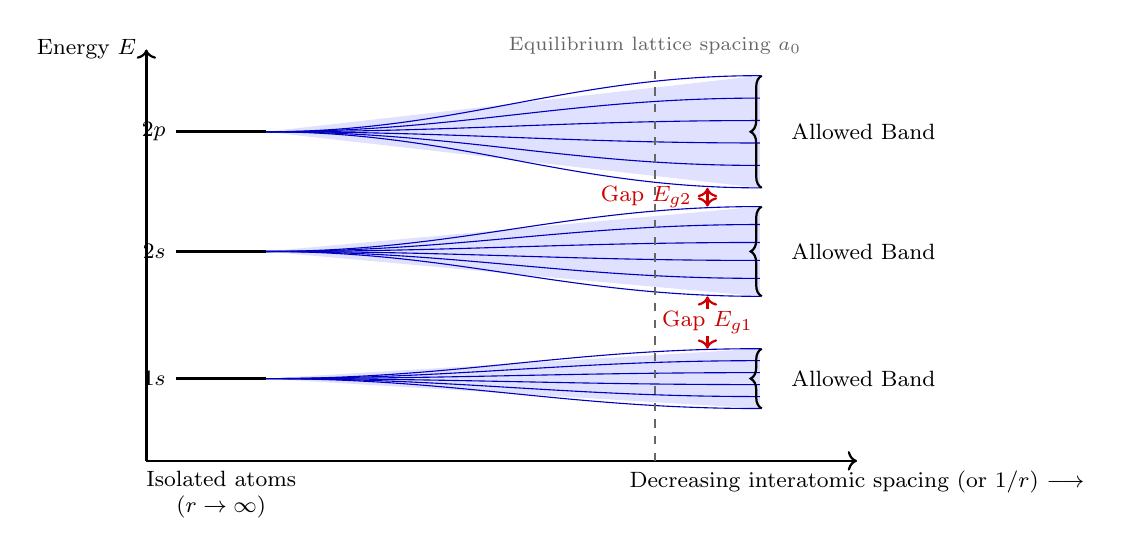
\begin{tikzpicture}[scale=0.95]
    \draw[->,thick] (0,0) -- (9.5,0) node[below,font=\footnotesize] {Decreasing interatomic spacing (or $1/r$) $\longrightarrow$};
    \draw[->,thick] (0,0) -- (0,5.5) node[left,font=\footnotesize] {Energy $E$};
    \draw[very thick] (0.4,1.1) -- (1.6,1.1) node[left,pos=0,font=\footnotesize] {$1s$};
    \draw[very thick] (0.4,2.8) -- (1.6,2.8) node[left,pos=0,font=\footnotesize] {$2s$};
    \draw[very thick] (0.4,4.4) -- (1.6,4.4) node[left,pos=0,font=\footnotesize] {$2p$};
    \node[font=\footnotesize,align=center] at (1.0,-0.45) {Isolated atoms\\($r \to \infty$)};
    \foreach \ylevel/\spread in {1.1/0.4, 2.8/0.6, 4.4/0.75}{
        \fill[blue!12] (1.6,\ylevel) -- (8.2,{\ylevel-\spread}) -- (8.2,{\ylevel+\spread}) -- cycle;
        \foreach \fval in {-1.0,-0.6,-0.2,0.2,0.6,1.0}{
            \draw[blue!75!black,thin] (1.6,\ylevel) to[out=0,in=180] (8.2,{\ylevel+\fval*\spread});
        }
        \draw[decorate,decoration={brace,amplitude=4pt,raise=2pt},thick]
            (8.3,{\ylevel-\spread}) -- (8.3,{\ylevel+\spread})
            node[midway,right=5pt,font=\footnotesize]{Allowed Band};
    }
    \draw[<->,red!80!black,thick] (7.5,1.5) -- (7.5,2.2) node[midway,fill=white,inner sep=1pt,font=\footnotesize]{Gap $E_{g1}$};
    \draw[<->,red!80!black,thick] (7.5,3.4) -- (7.5,3.65) node[midway,left=2pt,font=\footnotesize]{Gap $E_{g2}$};
    \draw[dashed,thick,gray!80!black] (6.8,0) -- (6.8,5.3) node[above,font=\scriptsize]{Equilibrium lattice spacing $a_0$};
\end{tikzpicture}
\caption{Splitting of discrete atomic energy levels ($1s, 2s, 2p$) into quasi-continuous allowed energy bands separated by forbidden energy gaps as $N \sim 10^{23}$ atoms assemble into a crystal.}
\label{fig:band_broadening_master}
\end{figure}

\subsection{Statement and Complete Proofs of Bloch's Theorem}
\textbf{Statement of Bloch's Theorem:} The eigenfunctions of the single-electron time-independent Schr\"odinger equation in a periodic potential,
\begin{equation}
    \mathcal{H}\psi(\rvec) = \left[-\frac{\hbarsq}{2m}\nabla^2 + V(\rvec)\right]\psi(\rvec) = E\psi(\rvec), \qquad V(\rvec + \RR_n) = V(\rvec),
    \label{eq:schrodinger_bloch}
\end{equation}
can always be chosen to take the form of a plane wave $e^{i\kk\cdot\rvec}$ modulated by a function $u_{\kk}(\rvec)$ that possesses the exact spatial periodicity of the crystal Bravais lattice:
\begin{equation}
    \boxed{\psi_{n\kk}(\rvec) = e^{i\kk\cdot\rvec}u_{n\kk}(\rvec), \qquad u_{n\kk}(\rvec + \RR_n) = u_{n\kk}(\rvec).}
    \label{eq:bloch_form1}
\end{equation}
Equivalently, under any crystal lattice translation $\rvec \to \rvec + \RR_n$:
\begin{equation}
    \boxed{\psi_{n\kk}(\rvec + \RR_n) = e^{i\kk\cdot\RR_n}\psi_{n\kk}(\rvec).}
    \label{eq:bloch_form2}
\end{equation}
Here $\kk$ is the **crystal wavevector**, $\hb\kk$ is the **crystal momentum**, and $n = 1, 2, 3, \dots$ is the **band index**.

\subsubsection{Proof 1: Exact Fourier Expansion and the Central Equation (Valid for Degenerate States)}
\begin{methodbox}{Derivation of the Central Equation and Bloch's Theorem}
\textbf{Step 1: Fourier expansion of the periodic potential $V(\rvec)$.}
Because $V(\rvec + \RR_n) = V(\rvec)$ for every direct lattice vector $\RR_n$, its Fourier expansion contains exclusively reciprocal lattice vectors $\GG$ (for which $\GG\cdot\RR_n = 2\pi \times \text{integer} \implies e^{i\GG\cdot\RR_n} = 1$):
\begin{equation}
    V(\rvec) = \sum_{\GG} V_{\GG} e^{i\GG\cdot\rvec}, \qquad V_{\GG} = \frac{1}{\Omega_{\mathrm{cell}}}\int_{\mathrm{cell}} V(\rvec)e^{-i\GG\cdot\rvec}\,\dd^3 r.
    \label{eq:VG_fourier_def}
\end{equation}
Because $V(\rvec)$ is real ($V^*(\rvec) = V(\rvec)$), its Fourier coefficients obey $V_{-\GG} = V_{\GG}^*$. If the crystal also possesses inversion symmetry $V(-\rvec) = V(\rvec)$, then $V_{\GG} = V_{-\GG} = V_{\GG}^*$ is purely real.

\textbf{Step 2: Fourier plane-wave expansion of the wavefunction $\psi(\rvec)$.}
We expand the unknown wavefunction $\psi(\rvec)$ over the complete orthonormal set of plane waves permitted by Born--von K\'arm\'an periodic boundary conditions over the crystal volume $\Omega$:
\begin{equation}
    \psi(\rvec) = \sum_{\kk} C(\kk) e^{i\kk\cdot\rvec},
\end{equation}
where $\kk = \frac{2\pi n_x}{L_x}\hat{\vb{x}} + \frac{2\pi n_y}{L_y}\hat{\vb{y}} + \frac{2\pi n_z}{L_z}\hat{\vb{z}}$ runs over all wavevectors allowed by the boundary conditions (not yet restricted to the first Brillouin zone).

\textbf{Step 3: Substitution into the Schr\"odinger equation.}
Acting with the kinetic energy operator gives $-\frac{\hbarsq}{2m}\nabla^2\psi(\rvec) = \sum_{\kk}\frac{\hbarsq k^2}{2m}C(\kk)e^{i\kk\cdot\rvec}$. Multiplying $V(\rvec)$ and $\psi(\rvec)$ gives:
\begin{equation}
    \sum_{\kk}\frac{\hbarsq k^2}{2m}C(\kk)e^{i\kk\cdot\rvec} + \sum_{\kk}\sum_{\GG} V_{\GG} C(\kk) e^{i(\kk+\GG)\cdot\rvec} = E \sum_{\kk} C(\kk) e^{i\kk\cdot\rvec}.
    \label{eq:central_sub}
\end{equation}

\textbf{Step 4: Shifting the dummy summation index in the potential term.}
In the double sum $\sum_{\kk}\sum_{\GG} V_{\GG} C(\kk) e^{i(\kk+\GG)\cdot\rvec}$, introduce the shifted wavevector $\kk' \equiv \kk + \GG$ (so $\kk = \kk' - \GG$). Because $\GG$ is a reciprocal lattice vector, shifting by $\GG$ simply permutes the allowed Born--von K\'arm\'an wavevectors. Renaming the dummy summation variable $\kk' \to \kk$ afterwards gives:
\begin{equation}
    \sum_{\kk}\sum_{\GG} V_{\GG} C(\kk) e^{i(\kk+\GG)\cdot\rvec} = \sum_{\kk'}\sum_{\GG} V_{\GG} C(\kk'-\GG) e^{i\kk'\cdot\rvec} = \sum_{\kk}\sum_{\GG} V_{\GG} C(\kk-\GG) e^{i\kk\cdot\rvec}.
\end{equation}
Now every term in Eq.~\eqref{eq:central_sub} carries the common phase factor $e^{i\kk\cdot\rvec}$:
\begin{equation}
    \sum_{\kk} \left[ \left(\frac{\hbarsq k^2}{2m} - E\right) C(\kk) + \sum_{\GG} V_{\GG} C(\kk-\GG) \right] e^{i\kk\cdot\rvec} = 0.
\end{equation}

\textbf{Step 5: Orthogonality of plane waves and the Central Equation.}
Multiplying both sides by $e^{-i\kk''\cdot\rvec}$ and integrating over the crystal volume $\Omega$ (using $\frac{1}{\Omega}\int_{\Omega} e^{i(\kk-\kk'')\cdot\rvec}\,\dd^3 r = \delta_{\kk,\kk''}$) isolates the $\kk = \kk''$ coefficient. Defining the free-electron kinetic energy $\lambda_{\kk} \equiv \frac{\hbarsq k^2}{2m}$, we obtain the **Central Equation**:
\begin{equation}
    \boxed{\left(\lambda_{\kk} - E\right)C(\kk) + \sum_{\GG} V_{\GG} C(\kk-\GG) = 0, \qquad \lambda_{\kk} = \frac{\hbarsq k^2}{2m}.}
    \label{eq:central_eq_master}
\end{equation}

\textbf{Step 6: Recovery of the Bloch wavefunction.}
Equation~\eqref{eq:central_eq_master} reveals that the Fourier coefficient $C(\kk)$ is coupled \emph{only} to coefficients $C(\kk-\GG)$ whose wavevectors differ from $\kk$ by a reciprocal lattice vector $\GG$. Thus, the infinite system of equations breaks up into $N$ independent decoupled blocks, one for each wavevector $\kk$ in the first Brillouin zone! An eigenstate belonging to block $\kk$ is constructed solely from the subset $\{\kk-\GG\}$:
\begin{equation}
    \psi_{\kk}(\rvec) = \sum_{\GG} C(\kk-\GG) e^{i(\kk-\GG)\cdot\rvec} = e^{i\kk\cdot\rvec} \underbrace{\left[ \sum_{\GG} C(\kk-\GG) e^{-i\GG\cdot\rvec} \right]}_{\equiv\, u_{\kk}(\rvec)}.
\end{equation}
Checking the translational invariance of $u_{\kk}(\rvec)$ under $\rvec \to \rvec + \RR_n$ (using $e^{-i\GG\cdot\RR_n} = 1$):
\begin{equation}
    u_{\kk}(\rvec + \RR_n) = \sum_{\GG} C(\kk-\GG) e^{-i\GG\cdot(\rvec + \RR_n)} = \sum_{\GG} C(\kk-\GG) e^{-i\GG\cdot\rvec} \underbrace{e^{-i\GG\cdot\RR_n}}_{=1} = u_{\kk}(\rvec).
\end{equation}
Thus $\psi_{\kk}(\rvec) = e^{i\kk\cdot\rvec}u_{\kk}(\rvec)$ with $u_{\kk}(\rvec + \RR_n) = u_{\kk}(\rvec)$, completing the exact proof of Bloch's theorem. $\blacksquare$
\end{methodbox}

\subsubsection{Proof 2: Translation Operator on a Ring of \texorpdfstring{$N$}{N} Atoms and State Counting}
Consider a 1D ring of $N$ identical lattice sites separated by lattice spacing $a$ (total length $L = Na$). Define the lattice translation operator $\hat{T}_a$ by $\hat{T}_a f(x) = f(x+a)$. Because $V(x+a) = V(x)$, $\hat{T}_a$ commutes with the Hamiltonian $\mathcal{H}$:
\begin{equation}
    [\mathcal{H}, \hat{T}_a]\psi(x) = \mathcal{H}\psi(x+a) - \hat{T}_a[\mathcal{H}(x)\psi(x)] = \mathcal{H}(x+a)\psi(x+a) - \mathcal{H}(x+a)\psi(x+a) = 0.
\end{equation}
Since $[\mathcal{H}, \hat{T}_a] = 0$, we can choose simultaneous eigenstates of $\mathcal{H}$ and $\hat{T}_a$:
\begin{equation}
    \hat{T}_a \psi(x) = \psi(x+a) = C\psi(x).
\end{equation}
Applying the translation operator $N$ times takes us once completely around the ring back to the starting point $x$. Single-valuedness of the wavefunction requires:
\begin{equation}
    \psi(x + Na) = C^N \psi(x) = \psi(x) \implies C^N = 1.
\end{equation}
Thus $C$ must be one of the $N$ complex roots of unity:
\begin{equation}
    C = \exp\left(\frac{i 2\pi s}{N}\right) = e^{ika}, \qquad \text{where } k = \frac{2\pi s}{Na} \quad (s = 0, \pm 1, \pm 2, \dots).
    \label{eq:allowed_k_ring}
\end{equation}
Writing $\psi_k(x) = e^{ikx}u_k(x)$, we check the periodicity of $u_k(x)$:
\begin{equation}
    u_k(x+a) = e^{-ik(x+a)}\psi_k(x+a) = e^{-ikx}e^{-ika}\left[e^{ika}\psi_k(x)\right] = e^{-ikx}\psi_k(x) = u_k(x). \quad \blacksquare
\end{equation}

\paragraph{Fundamental State-Counting Theorem per Band:}
From Eq.~\eqref{eq:allowed_k_ring}, the spacing between adjacent allowed $k$-values is $\Delta k = \frac{2\pi}{Na}$. Because $k$ and $k + \frac{2\pi}{a}$ produce the exact same eigenvalue $e^{ika}$, all physically distinct wavevectors lie within the **First Brillouin Zone** $-\frac{\pi}{a} < k \le +\frac{\pi}{a}$ of width $\frac{2\pi}{a}$. The total number of distinct orbital $\kk$-states in a single energy band is:
\begin{equation}
    N_k = \frac{\text{Width of 1st BZ}}{\Delta k} = \frac{2\pi/a}{2\pi/(Na)} = N \text{ orbital } \kk\text{-states per band}.
\end{equation}
Including the two spin orientations ($\ket{\uparrow}, \ket{\downarrow}$) per orbital state allowed by the Pauli exclusion principle:
\begin{equation}
    \boxed{\text{Total electron capacity of a single energy band} = 2N \text{ electrons} \quad (2 \text{ electrons per primitive unit cell}).}
    \label{eq:2N_capacity}
\end{equation}

\subsection{Time-Reversal Symmetry: Proof that \texorpdfstring{$E_n(-\kk) = E_n(\kk)$}{E_n(-k) = E_n(k)}}
\label{sec:time_reversal}
For a spinless electron in the absence of an external magnetic field, the crystal Hamiltonian $\mathcal{H} = -\frac{\hbarsq}{2m}\nabla^2 + V(\rvec)$ is a purely real operator ($\mathcal{H}^* = \mathcal{H}$). Taking the complex conjugate of the eigenvalue equation $\mathcal{H}\psi_{n\kk}(\rvec) = E_n(\kk)\psi_{n\kk}(\rvec)$ (since $E_n(\kk)$ is real) gives:
\begin{equation}
    \mathcal{H}\psi_{n\kk}^*(\rvec) = E_n(\kk)\psi_{n\kk}^*(\rvec).
\end{equation}
Thus $\psi_{n\kk}^*(\rvec)$ is also an eigenstate of $\mathcal{H}$ with the identical energy eigenvalue $E_n(\kk)$. Examining the translational property of $\psi_{n\kk}^*(\rvec)$:
\begin{equation}
    \psi_{n\kk}^*(\rvec) = \left[e^{i\kk\cdot\rvec}u_{n\kk}(\rvec)\right]^* = e^{i(-\kk)\cdot\rvec}u_{n\kk}^*(\rvec), \qquad \psi_{n\kk}^*(\rvec + \RR_n) = e^{i(-\kk)\cdot\RR_n}\psi_{n\kk}^*(\rvec).
\end{equation}
This shows that $\psi_{n\kk}^*(\rvec)$ is a Bloch state with wavevector $-\kk$. Therefore, the energy dispersion of any band is an even function of $\kk$:
\begin{equation}
    \boxed{E_n(-\kk) = E_n(\kk).}
\end{equation}
\textit{Note:} This holds even in crystals that lack spatial inversion symmetry (such as $\text{GaAs}$), because it is a consequence of **time-reversal symmetry** ($\mathcal{H}^* = \mathcal{H}$).

\begin{examplebox}{Free-Electron Plane Wave and Complex Conjugate Bloch States}{ex:bloch_basics}
\textbf{Problem.} (a) Show that the free-electron plane wave $\psi_{\kk}(\rvec) = \frac{1}{\sqrt{\Omega}}e^{i\kk\cdot\rvec}$ satisfies Bloch's theorem and identify $u_{\kk}(\rvec)$. (b) If a crystal contains $2.5 \times 10^{22}$ primitive unit cells, how many distinct $\kk$-states exist in the 1st Brillouin zone, and how many electrons can fill a single energy band?
\vspace{0.2cm}\hrule\vspace{0.2cm}
\textbf{Solution.}
\textbf{(a)} Comparing $\psi_{\kk}(\rvec) = e^{i\kk\cdot\rvec}\left(\frac{1}{\sqrt{\Omega}}\right)$ with Eq.~\eqref{eq:bloch_form1}, the cell-periodic function is the constant $u_{\kk}(\rvec) = \frac{1}{\sqrt{\Omega}}$, which trivially satisfies $u_{\kk}(\rvec + \RR_n) = u_{\kk}(\rvec)$. Under translation, $\psi_{\kk}(\rvec + \RR_n) = \frac{1}{\sqrt{\Omega}}e^{i\kk\cdot(\rvec+\RR_n)} = e^{i\kk\cdot\RR_n}\psi_{\kk}(\rvec)$.\\
\textbf{(b)} The number of distinct $\kk$-points in the 1st BZ equals the number of primitive cells: $N_k = N = \mathbf{2.5 \times 10^{22}}$. Including spin degeneracy ($g_s = 2$), a single energy band holds $2N = \mathbf{5.0 \times 10^{22}\ \text{electrons}}$.
\end{examplebox}

% ============================================================================
\section{The Nearly Free Electron (NFE) Model and Origin of Energy Bands}
\label{sec:nfe}
% ============================================================================

\subsection{Hamiltonian Setup and Reciprocal-Space Scattering Matrix Elements}
In the **Nearly Free Electron (NFE) model**, we partition the single-electron Hamiltonian into the free-electron kinetic energy $\hat{H}_0$ and a weak periodic lattice potential $\hat{V}(\rvec)$:
\begin{equation}
    \hat{H} = \hat{H}_0 + \hat{V}(\rvec), \qquad \hat{H}_0 = -\frac{\hbarsq}{2m}\nabla^2, \qquad \hat{H}_0\ket{\kk} = \Ebare(\kk)\ket{\kk} = \frac{\hbarsq k^2}{2m}\ket{\kk},
\end{equation}
where $\braket{\rvec}{\kk} = \frac{1}{\sqrt{\Omega}}e^{i\kk\cdot\rvec}$ are normalized plane waves obeying $\braket{\kpvec}{\kk} = \delta_{\kpvec,\kk}$.

Substituting the Fourier series $V(\rvec) = \sum_{\GG} V_{\GG} e^{i\GG\cdot\rvec}$ into the matrix element between two plane waves $\ket{\kk}$ and $\ket{\kpvec}$ gives the **reciprocal-lattice scattering selection rule**:
\begin{align}
    \mel{\kpvec}{V}{\kk} &= \frac{1}{\Omega}\int_{\Omega} e^{-i\kpvec\cdot\rvec} \left( \sum_{\GG} V_{\GG} e^{i\GG\cdot\rvec} \right) e^{i\kk\cdot\rvec}\,\dd^3 r \notag\\
    &= \sum_{\GG} V_{\GG} \left( \frac{1}{\Omega}\int_{\Omega} e^{i(\kk + \GG - \kpvec)\cdot\rvec}\,\dd^3 r \right) = \sum_{\GG} V_{\GG} \delta_{\kpvec, \kk+\GG}.
    \label{eq:nfe_selection_rule}
\end{align}
Thus, the periodic potential scatters an electron from $\kk$ to $\kpvec$ **if and only if** the momentum transfer equals a reciprocal lattice vector: $\kpvec - \kk = \GG$.

\subsection{Non-Degenerate Perturbation Theory and Breakdown at Zone Boundaries}
Applying standard Rayleigh--Schr\"odinger non-degenerate perturbation theory up to second order in $V$:
\begin{equation}
    E(\kk) = \Ebare(\kk) + \mel{\kk}{V}{\kk} + \sum_{\kpvec \neq \kk} \frac{\abs{\mel{\kpvec}{V}{\kk}}^2}{\Ebare(\kk) - \Ebare(\kpvec)} + \mathcal{O}(V^3).
\end{equation}
\begin{enumerate}
    \item \textbf{Why First-Order Perturbation Theory Gives No Dispersion or Band Gap:}
    The first-order energy shift is the diagonal expectation value:
    \begin{equation}
        E_{\kk}^{(1)} = \mel{\kk}{V}{\kk} = \frac{1}{\Omega}\int_{\Omega} e^{-i\kk\cdot\rvec} V(\rvec) e^{i\kk\cdot\rvec}\,\dd^3 r = \frac{1}{\Omega}\int_{\Omega} V(\rvec)\,\dd^3 r = V_{\GG=\vb{0}} \equiv V_0.
    \end{equation}
    Physically, a running plane wave has a completely uniform probability density $\abs{\psi_{\kk}^{(0)}(\rvec)}^2 = 1/\Omega$, so it samples all parts of the unit cell equally and only feels the spatial average $V_0$ of the potential. Since $V_0$ is independent of $\kk$, it merely shifts all energies rigidly and can be set to zero ($V_0 \equiv 0$) by choice of energy origin.
    \item \textbf{Second-Order Energy Shift and Divergence at Bragg Planes:}
    Using the selection rule~\eqref{eq:nfe_selection_rule}, the second-order expansion becomes:
    \begin{equation}
        \boxed{E(\kk) = \Ebare(\kk) + V_0 + \sum_{\GG \neq \vb{0}} \frac{\abs{V_{\GG}}^2}{\Ebare(\kk) - \Ebare(\kk+\GG)}.}
        \label{eq:nfe_2nd_order_master}
    \end{equation}
    The energy denominator in Eq.~\eqref{eq:nfe_2nd_order_master} vanishes whenever the scattered state $\ket{\kk+\GG}$ is degenerate with $\ket{\kk}$:
    \begin{equation}
        \Ebare(\kk) = \Ebare(\kk+\GG) \iff \frac{\hbarsq k^2}{2m} = \frac{\hbarsq \abs{\kk+\GG}^2}{2m} \iff 2\kk\cdot\GG + G^2 = 0 \iff \kk\cdot\hat{\GG} = -\frac{1}{2}\abs{\GG}.
    \end{equation}
    This is the exact **Laue / Bragg diffraction condition** defining the **Brillouin zone boundary** (in 1D, $k = \pm \frac{G}{2} = \pm \frac{n\pi}{a}$). At and near these zone boundaries, non-degenerate perturbation theory breaks down completely, and we must use **degenerate perturbation theory**.
\end{enumerate}

\subsection{Degenerate Perturbation Theory: The Two-Band Secular Equation}
When $\kk$ lies on or near a Brillouin zone boundary such that $\Ebare(\kk) \approx \Ebare(\kk+\GG)$ (or equivalently $\Ebare(\kk) \approx \Ebare(\kk-\GG)$), we isolate the two strongly coupled plane-wave states $\ket{\kk}$ and $\ket{\kk-\GG}$ and write the trial wavefunction:
\begin{equation}
    \ket{\psi_{\kk}} = C(\kk)\ket{\kk} + C(\kk-\GG)\ket{\kk-\GG}.
\end{equation}
Projecting $\hat{H}\ket{\psi_{\kk}} = E\ket{\psi_{\kk}}$ onto $\bra{\kk}$ and $\bra{\kk-\GG}$ (setting $V_0 = 0$ and denoting $U \equiv V_{\GG} = V_{-\GG}^*$) yields the $2\times 2$ matrix eigenvalue problem (equivalently obtained by truncating the Central Equation~\eqref{eq:central_eq_master} to two terms):
\begin{equation}
    \begin{pmatrix}
        \lambda_{\kk} - E & U \\
        U^* & \lambda_{\kk-\GG} - E
    \end{pmatrix}
    \begin{pmatrix}
        C(\kk) \\
        C(\kk-\GG)
    \end{pmatrix}
    =
    \begin{pmatrix}
        0 \\
        0
    \end{pmatrix},
    \qquad \text{where } \lambda_{\kk} \equiv \Ebare(\kk) = \frac{\hbarsq k^2}{2m}.
    \label{eq:nfe_2x2_system}
\end{equation}
Setting the $2\times 2$ determinant to zero gives the secular quadratic equation:
\begin{equation}
    (\lambda_{\kk} - E)(\lambda_{\kk-\GG} - E) - \abs{U}^2 = E^2 - (\lambda_{\kk} + \lambda_{\kk-\GG})E + \lambda_{\kk}\lambda_{\kk-\GG} - \abs{U}^2 = 0.
\end{equation}
Solving for $E$ yields the exact two-band NFE dispersion relation:
\begin{equation}
    \boxed{E_\pm(\kk) = \frac{\lambda_{\kk} + \lambda_{\kk-\GG}}{2} \pm \sqrt{\left(\frac{\lambda_{\kk} - \lambda_{\kk-\GG}}{2}\right)^2 + \abs{V_{\GG}}^2}.}
    \label{eq:nfe_general_dispersion}
\end{equation}

\subsubsection{Energy Gap directly at the Brillouin Zone Boundary}
Directly on the Brillouin zone boundary ($k = \pm \pi/a$ in 1D), the two unperturbed states are strictly degenerate: $\lambda_{\kk} = \lambda_{\kk-\GG} \equiv \lambda = \frac{\hbarsq(\pi/a)^2}{2m}$. Equation~\eqref{eq:nfe_general_dispersion} reduces immediately to:
\begin{equation}
    E_\pm\left(\frac{\pi}{a}\right) = \lambda \pm \abs{V_G} \implies \boxed{E_g = E_+ - E_- = 2\abs{V_G}.}
    \label{eq:nfe_gap_master}
\end{equation}
Thus, the periodic potential lifts the degeneracy at the $n$-th Brillouin zone boundary $k = \pm n\pi/a$ and opens a **forbidden energy gap** equal to twice the magnitude of the $n$-th Fourier harmonic $V_{G_n}$ of the potential!

\subsubsection{Parabolic Expansion and Zero Slope Near the Zone Boundary}
Let us expand Eq.~\eqref{eq:nfe_general_dispersion} in 1D just inside the zone boundary by setting $k = \frac{G}{2} - K = \frac{\pi}{a} - K$ with $\abs{K} \ll \frac{\pi}{a}$, so that $k - G = -\left(\frac{G}{2} + K\right)$. The unperturbed kinetic energies are (with $\lambda = \frac{\hbarsq (G/2)^2}{2m}$):
\begin{align}
    \lambda_k &= \frac{\hbarsq}{2m}\left(\frac{G}{2} - K\right)^2 = \lambda - \frac{\hbarsq G K}{2m} + \frac{\hbarsq K^2}{2m}, \\
    \lambda_{k-G} &= \frac{\hbarsq}{2m}\left(\frac{G}{2} + K\right)^2 = \lambda + \frac{\hbarsq G K}{2m} + \frac{\hbarsq K^2}{2m}.
\end{align}
Computing the half-sum and half-difference squared:
\begin{equation}
    \frac{\lambda_k + \lambda_{k-G}}{2} = \lambda + \frac{\hbarsq K^2}{2m}, \qquad \left(\frac{\lambda_k - \lambda_{k-G}}{2}\right)^2 = \left(\frac{\hbarsq G K}{2m}\right)^2 = 4\lambda\left(\frac{\hbarsq K^2}{2m}\right).
\end{equation}
Substituting these into Eq.~\eqref{eq:nfe_general_dispersion} and Taylor-expanding $\sqrt{1 + x} \approx 1 + \frac{1}{2}x$ for small $K$:
\begin{align}
    E_\pm(K) &= \lambda + \frac{\hbarsq K^2}{2m} \pm \abs{U}\sqrt{1 + \frac{4\lambda}{\abs{U}^2}\left(\frac{\hbarsq K^2}{2m}\right)} \notag\\
    &\approx \lambda + \frac{\hbarsq K^2}{2m} \pm \abs{U}\left[ 1 + \frac{2\lambda}{\abs{U}^2}\left(\frac{\hbarsq K^2}{2m}\right) \right] \notag\\
    \Aboxed{E_\pm(K) &= (\lambda \pm \abs{U}) + \frac{\hbarsq K^2}{2m}\left(1 \pm \frac{2\lambda}{\abs{U}}\right).}
    \label{eq:nfe_parabolic_edge}
\end{align}
\begin{itemize}
    \item \textbf{Zero Group Velocity at Zone Boundaries:} Because the linear term in $K$ vanishes, $\left.\dv{E_\pm}{k}\right|_{k=\pm\pi/a} = 0$, proving that energy bands always intersect the Brillouin zone boundaries horizontally with zero slope!
    \item \textbf{Band-Edge Effective Mass Enhancement:} Differentiating twice with respect to $K$ gives the effective mass at the band edges:
    \begin{equation}
        \boxed{\frac{m_\pm^*}{m} = \frac{1}{1 \pm \frac{2\lambda}{\abs{U}}} = \frac{1}{1 \pm \frac{4\lambda}{E_g}}.}
        \label{eq:nfe_mstar_formula}
    \end{equation}
\end{itemize}

\begin{figure}[htbp]
\centering
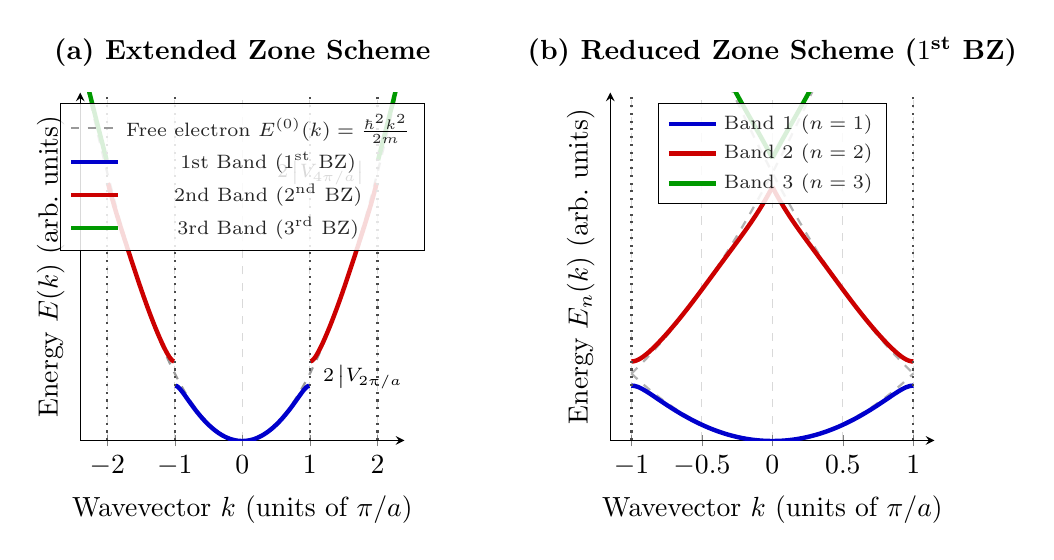
\begin{tikzpicture}
  % ---------------- LEFT PLOT: EXTENDED ZONE SCHEME ----------------
  \begin{axis}[
    name=extended_plot,
    width=0.47\textwidth,
    height=6.0cm,
    title={\textbf{(a) Extended Zone Scheme}},
    xlabel={Wavevector $k$ (units of $\pi/a$)},
    ylabel={Energy $E(k)$ (arb.\ units)},
    xmin=-2.4, xmax=2.4,
    ymin=0, ymax=5.2,
    xtick={-2,-1,0,1,2},
    xticklabels={$-2$,$-1$,$0$,$1$,$2$},
    ytick=\empty,
    axis lines=left,
    grid=major,
    grid style={dashed,gray!30},
    legend style={at={(0.5,0.97)},anchor=north,font=\scriptsize,fill=white,fill opacity=0.85}
  ]
    \addplot[domain=-2.3:2.3, samples=100, dashed, gray!80, thick] {x^2};
    \addlegendentry{Free electron $\Ebare(k)=\frac{\hbarsq k^2}{2m}$}
    
    \addplot[domain=-0.99:0.99, samples=80, blue!80!black, ultra thick] {0.5*(x^2 + (abs(x)-2)^2) - sqrt(0.25*(x^2 - (abs(x)-2)^2)^2 + 0.18^2)};
    \addlegendentry{1st Band ($1^{\text{st}}$ BZ)}
    
    \addplot[domain=-1.99:-1.01, samples=60, red!80!black, ultra thick, forget plot] {0.5*(x^2 + (x+2)^2) + sqrt(0.25*(x^2 - (x+2)^2)^2 + 0.18^2) - 0.12*exp(-15*(x+2)^2)};
    \addplot[domain=1.01:1.99, samples=60, red!80!black, ultra thick] {0.5*(x^2 + (x-2)^2) + sqrt(0.25*(x^2 - (x-2)^2)^2 + 0.18^2) - 0.12*exp(-15*(x-2)^2)};
    \addlegendentry{2nd Band ($2^{\text{nd}}$ BZ)}

    \addplot[domain=-2.3:-2.01, samples=30, green!60!black, ultra thick, forget plot] {x^2 + 0.15*exp(-10*(x+2)^2)};
    \addplot[domain=2.01:2.3, samples=30, green!60!black, ultra thick] {x^2 + 0.15*exp(-10*(x-2)^2)};
    \addlegendentry{3rd Band ($3^{\text{rd}}$ BZ)}

    \draw[dotted, thick, black!70] (axis cs:-1,0) -- (axis cs:-1,5.2);
    \draw[dotted, thick, black!70] (axis cs:1,0) -- (axis cs:1,5.2);
    \draw[dotted, thick, black!70] (axis cs:-2,0) -- (axis cs:-2,5.2);
    \draw[dotted, thick, black!70] (axis cs:2,0) -- (axis cs:2,5.2);

    \node[anchor=west, font=\scriptsize\bfseries, text=black] at (axis cs:1.05, 0.95) {$2\abs{V_{2\pi/a}}$};
    \node[anchor=east, font=\scriptsize\bfseries, text=black] at (axis cs:1.95, 4.0) {$2\abs{V_{4\pi/a}}$};
  \end{axis}

  % ---------------- RIGHT PLOT: REDUCED ZONE SCHEME ----------------
  \begin{axis}[
    name=reduced_plot,
    at={(extended_plot.right of south east)},
    anchor=left of south west,
    xshift=1.0cm,
    width=0.47\textwidth,
    height=6.0cm,
    title={\textbf{(b) Reduced Zone Scheme ($1^{\text{st}}$ BZ)}},
    xlabel={Wavevector $k$ (units of $\pi/a$)},
    ylabel={Energy $E_n(k)$ (arb.\ units)},
    xmin=-1.15, xmax=1.15,
    ymin=0, ymax=5.2,
    xtick={-1,-0.5,0,0.5,1},
    xticklabels={$-1$,$-0.5$,$0$,$0.5$,$1$},
    ytick=\empty,
    axis lines=left,
    grid=major,
    grid style={dashed,gray!30},
    legend style={at={(0.5,0.97)},anchor=north,font=\scriptsize,fill=white,fill opacity=0.85}
  ]
    \addplot[domain=-1:1, samples=60, dashed, gray!60, thick, forget plot] {x^2};
    \addplot[domain=-1:1, samples=60, dashed, gray!60, thick, forget plot] {(x-2)^2};
    \addplot[domain=-1:1, samples=60, dashed, gray!60, thick, forget plot] {(x+2)^2};

    \addplot[domain=-1:1, samples=80, blue!80!black, ultra thick] {0.5*(x^2 + (abs(x)-2)^2) - sqrt(0.25*(x^2 - (abs(x)-2)^2)^2 + 0.18^2)};
    \addlegendentry{Band 1 ($n=1$)}

    \addplot[domain=-1:0, samples=60, red!80!black, ultra thick, forget plot] {0.5*(x^2 + (x+2)^2) + sqrt(0.25*(x^2 - (x+2)^2)^2 + 0.18^2) - 0.22*exp(-12*x^2)};
    \addplot[domain=0:1, samples=60, red!80!black, ultra thick] {0.5*(x^2 + (x-2)^2) + sqrt(0.25*(x^2 - (x-2)^2)^2 + 0.18^2) - 0.22*exp(-12*x^2)};
    \addlegendentry{Band 2 ($n=2$)}

    \addplot[domain=-1:0, samples=60, green!60!black, ultra thick, forget plot] {(x-2)^2 + 0.22*exp(-12*x^2)};
    \addplot[domain=0:1, samples=60, green!60!black, ultra thick] {(x+2)^2 + 0.22*exp(-12*x^2)};
    \addlegendentry{Band 3 ($n=3$)}

    \draw[dotted, thick, black!70] (axis cs:-1,0) -- (axis cs:-1,5.2);
    \draw[dotted, thick, black!70] (axis cs:1,0) -- (axis cs:1,5.2);
  \end{axis}
\end{tikzpicture}
\caption{Dispersion relation $E(k)$ in the Nearly Free Electron model shown in \textbf{(a)} the Extended Zone Scheme and \textbf{(b)} the Reduced Zone Scheme, where outer segments of the perturbed parabola are folded by reciprocal lattice vectors $G = \pm 2\pi n/a$ into the First Brillouin Zone $[-\pi/a, \pi/a]$.}
\label{fig:zone_schemes_master}
\end{figure}

\subsection{Physical Origin of the Band Gap: Standing Waves and Electrostatic Energy}
Why do two states with identical wavevector magnitude $k = \pm\pi/a$ have an energy difference of $2\abs{V_{2\pi/a}}$? Consider a 1D crystal with positive ion cores at $x = 0, \pm a, \pm 2a, \dots$ creating an attractive periodic potential:
\begin{equation}
    V(x) = -2\tilde{V}\cos\left(\frac{2\pi x}{a}\right) = -\tilde{V}e^{i\frac{2\pi x}{a}} - \tilde{V}e^{-i\frac{2\pi x}{a}} \qquad (\tilde{V} > 0, \quad V_{\pm 2\pi/a} = -\tilde{V}).
\end{equation}
At $k = \pi/a$, Bragg reflection mixes $\frac{1}{\sqrt{L}}e^{i\pi x/a}$ and $\frac{1}{\sqrt{L}}e^{-i\pi x/a}$ with equal weight ($C(-\pi/a) = \pm C(\pi/a)$), forming two orthogonal **standing waves** (Figure~\ref{fig:standing_waves_master}):
\begin{align}
    \psi_+(x) &= \frac{1}{\sqrt{2L}}\left(e^{i\pi x/a} + e^{-i\pi x/a}\right) = \sqrt{\frac{2}{L}}\cos\left(\frac{\pi x}{a}\right) \implies \rho_+(x) = \abs{\psi_+(x)}^2 = \frac{2}{L}\cos^2\left(\frac{\pi x}{a}\right) = \frac{1}{L}\left[1 + \cos\left(\frac{2\pi x}{a}\right)\right], \\
    \psi_-(x) &= \frac{1}{i\sqrt{2L}}\left(e^{i\pi x/a} - e^{-i\pi x/a}\right) = \sqrt{\frac{2}{L}}\sin\left(\frac{\pi x}{a}\right) \implies \rho_-(x) = \abs{\psi_-(x)}^2 = \frac{2}{L}\sin^2\left(\frac{\pi x}{a}\right) = \frac{1}{L}\left[1 - \cos\left(\frac{2\pi x}{a}\right)\right].
\end{align}
Evaluating the expectation value of the potential energy $V(x)$ directly in real space for both standing waves:
\begin{align}
    \mel{\psi_+}{V(x)}{\psi_+} &= \int_0^L \left[-2\tilde{V}\cos\left(\frac{2\pi x}{a}\right)\right]\frac{1}{L}\left[1 + \cos\left(\frac{2\pi x}{a}\right)\right]\dd x = -\frac{2\tilde{V}}{L}\left(\frac{L}{2}\right) = -\tilde{V} \quad (\text{Lower Band Edge}), \\
    \mel{\psi_-}{V(x)}{\psi_-} &= \int_0^L \left[-2\tilde{V}\cos\left(\frac{2\pi x}{a}\right)\right]\frac{1}{L}\left[1 - \cos\left(\frac{2\pi x}{a}\right)\right]\dd x = +\frac{2\tilde{V}}{L}\left(\frac{L}{2}\right) = +\tilde{V} \quad (\text{Upper Band Edge}).
\end{align}
\begin{itemize}
    \item $\rho_+(x) \propto \cos^2(\pi x/a)$ piles electron probability density directly on top of the attractive positive ion cores at $x = na$, lowering its electrostatic potential energy by $-\tilde{V}$.
    \item $\rho_-(x) \propto \sin^2(\pi x/a)$ has nodes at the ion cores and concentrates electron probability in the interstitial regions $x = (n+\frac{1}{2})a$ between ions, raising its electrostatic energy by $+\tilde{V}$.
    \item The difference in electrostatic potential energy between the two standing waves is $E_g = (+\tilde{V}) - (-\tilde{V}) = 2\tilde{V} = 2\abs{V_{2\pi/a}}$.
\end{itemize}

\begin{figure}[htbp]
\centering
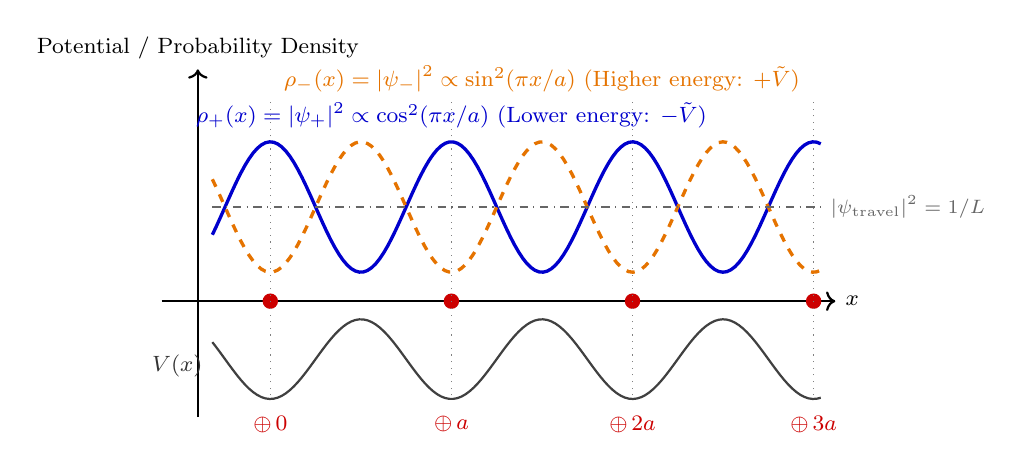
\begin{tikzpicture}[scale=0.92]
    \draw[->,thick] (-0.5,0) -- (8.8,0) node[right,font=\footnotesize] {$x$};
    \draw[->,thick] (0,-1.6) -- (0,3.2) node[above,font=\footnotesize] {Potential / Probability Density};
    \foreach \xion/\lab in {1.0/0, 3.5/a, 6.0/2a, 8.5/3a}{
        \filldraw[red!80!black] (\xion,0) circle (2.8pt);
        \node[below=4pt,font=\footnotesize,red!80!black] at (\xion,-1.3) {$\oplus\,\lab$};
        \draw[dotted,gray] (\xion,-1.3) -- (\xion,2.8);
    }
    \draw[thick,black!75,domain=0.2:8.6,samples=150] plot (\x, {-0.8 - 0.55*cos(360*(\x-1.0)/2.5)});
    \node[left,font=\footnotesize,black!80] at (0.2,-0.9) {$V(x)$};
    \draw[very thick,blue!80!black,domain=0.2:8.6,samples=150] plot (\x, {0.4 + 1.8*(cos(180*(\x-1.0)/2.5))^2});
    \node[above,font=\footnotesize,blue!80!black] at (3.5,2.25) {$\rho_+(x) = \abs{\psi_+}^2 \propto \cos^2(\pi x/a)$ (Lower energy: $-\tilde{V}$)};
    \draw[very thick,orange!90!black,dashed,domain=0.2:8.6,samples=150] plot (\x, {0.4 + 1.8*(sin(180*(\x-1.0)/2.5))^2});
    \node[above,font=\footnotesize,orange!90!black] at (4.75,2.75) {$\rho_-(x) = \abs{\psi_-}^2 \propto \sin^2(\pi x/a)$ (Higher energy: $+\tilde{V}$)};
    \draw[thin,gray!80!black,dashdotted] (0.2,1.3) -- (8.6,1.3) node[right,font=\scriptsize] {$\abs{\psi_{\mathrm{travel}}}^2 = 1/L$};
\end{tikzpicture}
\caption{Physical origin of the energy band gap $E_g = 2\abs{V_G}$ at $k = \pm\pi/a$: $\rho_+(x)$ piles electron density on the attractive positive ion cores, whereas $\rho_-(x)$ piles electron density between the ion cores.}
\label{fig:standing_waves_master}
\end{figure}

\begin{examplebox}{1D Cosine Potential Band Gap and Zone-Edge Energies}{ex:cosine_nfe}
\textbf{Problem.} A 1D crystal of lattice constant $a = 5.0\ \text{\AA}$ has periodic potential $V(x) = V_1\cos(2\pi x/a) + V_2\cos(4\pi x/a)$ with $V_1 = 1.00\ \mathrm{eV}$ and $V_2 = 0.40\ \mathrm{eV}$. Calculate (a) the first-order energy gaps at $k = \pi/a$ and $k = 2\pi/a$, and (b) the upper and lower band-edge energies $E_\pm(\pi/a)$.
\vspace{0.2cm}\hrule\vspace{0.2cm}
\textbf{Solution.}
\textbf{(a)} Using $\cos(Gx) = \frac{1}{2}(e^{iGx} + e^{-iGx})$, the Fourier coefficients are $V_{\pm 2\pi/a} = \frac{V_1}{2} = 0.50\ \mathrm{eV}$ and $V_{\pm 4\pi/a} = \frac{V_2}{2} = 0.20\ \mathrm{eV}$. Thus:
\[
    E_{g1}\left(k=\frac{\pi}{a}\right) = 2\abs{V_{2\pi/a}} = \mathbf{1.00\ \mathrm{eV}}, \qquad E_{g2}\left(k=\frac{2\pi}{a}\right) = 2\abs{V_{4\pi/a}} = \mathbf{0.40\ \mathrm{eV}}.
\]
\textbf{(b)} At $k = \frac{\pi}{5.0\ \text{\AA}} = 0.6283\ \text{\AA}^{-1}$, the unperturbed kinetic energy is $\lambda = \frac{\hbarsq k^2}{2m_e} = 3.81\ \mathrm{eV\cdot\text{\AA}^2}\times (0.6283\ \text{\AA}^{-1})^2 = 1.504\ \mathrm{eV}$. Therefore:
\[
    E_+\left(\frac{\pi}{a}\right) = 1.504 + 0.50 = \mathbf{2.004\ \mathrm{eV}}, \qquad E_-\left(\frac{\pi}{a}\right) = 1.504 - 0.50 = \mathbf{1.004\ \mathrm{eV}}.
\]
\end{examplebox}

\subsection{Extension to 3D Lattices: The FCC First Brillouin Zone and High-Symmetry Points}
In three dimensions, reciprocal lattice vectors $\GG$ define Bragg reflection planes $\kk \cdot \left(\frac{1}{2}\GG\right) = \left(\frac{1}{2}\GG\right)^2$ that bound the first Brillouin zone. For a **Face-Centered Cubic (FCC)** direct lattice of conventional lattice constant $a$ (the Bravais lattice of Diamond, Silicon, Germanium, and III--V semiconductors such as $\text{GaAs}$ and $\text{InP}$):
\begin{itemize}
    \item The reciprocal lattice is a **Body-Centered Cubic (BCC)** lattice with primitive translation vectors $\vb{b}_1 = \frac{2\pi}{a}(-\hat{\vb{x}}+\hat{\vb{y}}+\hat{\vb{z}})$, $\vb{b}_2 = \frac{2\pi}{a}(\hat{\vb{x}}-\hat{\vb{y}}+\hat{\vb{z}})$, $\vb{b}_3 = \frac{2\pi}{a}(\hat{\vb{x}}+\hat{\vb{y}}-\hat{\vb{z}})$.
    \item The first Brillouin zone is the Wigner--Seitz primitive cell of the reciprocal BCC lattice: a **truncated octahedron** bounded by $8$ regular hexagonal faces ($\{111\}$ planes) and $6$ square faces ($\{200\}$ planes) (Figure~\ref{fig:fcc_bz_truncated_octahedron_master}).
\end{itemize}
The standard high-symmetry points and lines connecting them index the electronic band structure $E(\kk)$:
\begin{itemize}
    \item \textbf{$\Gamma$-point (Zone Center):} $\kk_\Gamma = (0, 0, 0)$.
    \item \textbf{$X$-point (Center of Square Face along $[100]$):} $\kk_X = \frac{2\pi}{a}(1, 0, 0)$.
    \item \textbf{$L$-point (Center of Hexagonal Face along $[111]$):} $\kk_L = \frac{\pi}{a}(1, 1, 1)$.
    \item \textbf{$W$-point (Corner vertex where two hexagons and one square meet):} $\kk_W = \frac{\pi}{a}(2, 1, 0)$.
    \item \textbf{$K$-point (Center of edge joining two hexagonal faces):} $\kk_K = \frac{3\pi}{2a}(1, 1, 0)$.
\end{itemize}

\begin{figure}[htbp]
\centering
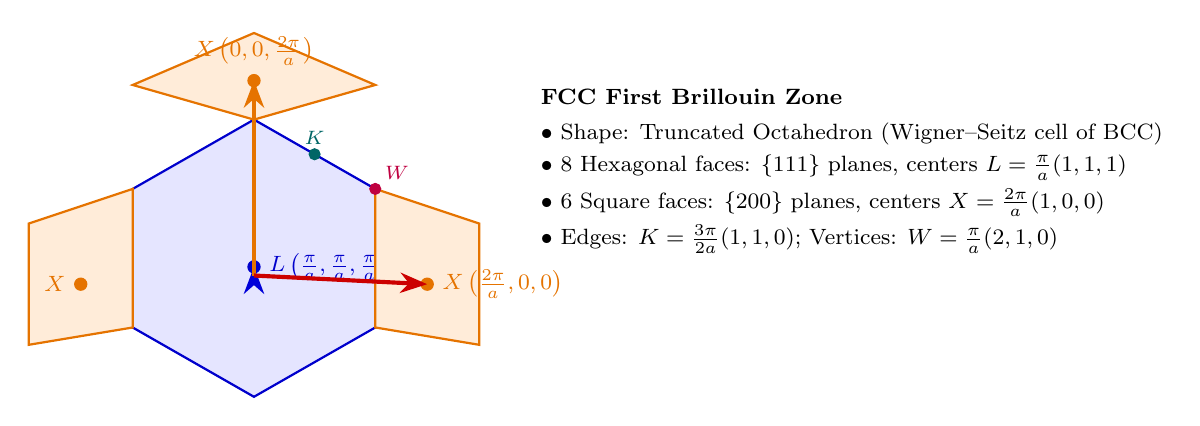
\begin{tikzpicture}[scale=1.1, >=Stealth]
  % Center Gamma
  \filldraw[black] (0,0) circle (2.5pt) node[below=2pt,font=\bfseries] {$\Gamma (0,0,0)$};

  % Front Hexagonal face (L point)
  \filldraw[fill=blue!10,draw=blue!80!black,thick]
    (0,1.8) -- (1.4,1.0) -- (1.4,-0.6) -- (0,-1.4) -- (-1.4,-0.6) -- (-1.4,1.0) -- cycle;
  \filldraw[blue!80!black] (0,0.1) circle (2pt) node[right=2pt,font=\footnotesize\bfseries] {$L \left(\frac{\pi}{a},\frac{\pi}{a},\frac{\pi}{a}\right)$};

  % Top Square Face (X point)
  \filldraw[fill=orange!15,draw=orange!90!black,thick]
    (0,1.8) -- (1.4,2.2) -- (0,2.8) -- (-1.4,2.2) -- cycle;
  \filldraw[orange!90!black] (0,2.25) circle (2pt) node[above=2pt,font=\footnotesize\bfseries] {$X \left(0,0,\frac{2\pi}{a}\right)$};

  % Right Square Face (X point)
  \filldraw[fill=orange!15,draw=orange!90!black,thick]
    (1.4,1.0) -- (2.6,0.6) -- (2.6,-0.8) -- (1.4,-0.6) -- cycle;
  \filldraw[orange!90!black] (2.0,-0.1) circle (2pt) node[right=2pt,font=\footnotesize\bfseries] {$X \left(\frac{2\pi}{a},0,0\right)$};

  % Left Square Face
  \filldraw[fill=orange!15,draw=orange!90!black,thick]
    (-1.4,1.0) -- (-2.6,0.6) -- (-2.6,-0.8) -- (-1.4,-0.6) -- cycle;
  \filldraw[orange!90!black] (-2.0,-0.1) circle (2pt) node[left=2pt,font=\footnotesize\bfseries] {$X$};

  % High symmetry vertices and edge points
  \filldraw[purple] (1.4,1.0) circle (1.8pt) node[above right,font=\scriptsize] {$W$};
  \filldraw[teal!80!black] (0.7,1.4) circle (1.8pt) node[above,font=\scriptsize] {$K$};

  % High-symmetry lines
  \draw[->,line width=1.5pt,blue!85!black] (0,0) -- (0,0.1);
  \draw[->,line width=1.5pt,orange!90!black] (0,0) -- (0,2.25);
  \draw[->,line width=1.5pt,red!80!black] (0,0) -- (2.0,-0.1);

  % Annotations
  \node[anchor=west,font=\footnotesize,align=left] at (3.2,1.2) {
    \textbf{FCC First Brillouin Zone}\\[3pt]
    $\bullet$ Shape: Truncated Octahedron (Wigner--Seitz cell of BCC)\\[2pt]
    $\bullet$ 8 Hexagonal faces: $\{111\}$ planes, centers $L = \frac{\pi}{a}(1,1,1)$\\[2pt]
    $\bullet$ 6 Square faces: $\{200\}$ planes, centers $X = \frac{2\pi}{a}(1,0,0)$\\[2pt]
    $\bullet$ Edges: $K = \frac{3\pi}{2a}(1,1,0)$; Vertices: $W = \frac{\pi}{a}(2,1,0)$
  };
\end{tikzpicture}
\caption{The First Brillouin Zone of the Face-Centered Cubic (FCC) lattice (truncated octahedron), illustrating the high-symmetry points $\Gamma$, $X$, $L$, $W$, and $K$ along which electronic band structures $E(\kk)$ are traditionally evaluated.}
\label{fig:fcc_bz_truncated_octahedron_master}
\end{figure}

% ============================================================================
\section{Energy Band Theory: Kronig--Penney Model and Tight-Binding Approximation}
\label{sec:kp_tb}
% ============================================================================

\subsection{The Kronig--Penney Model: Complete Unabridged Derivation}
Kronig and Penney (1931) modeled the 1D periodic crystal potential as an array of rectangular wells of width $a$ ($V = 0$) separated by rectangular barriers of width $b$ and height $V_0$, with spatial period $c = a + b$ (Figure~\ref{fig:kp_potential_master}):
\begin{equation}
    V(x) = \begin{cases}
        0, & 0 < x < a \quad \text{(Region I: Well)}, \\
        V_0, & -b < x < 0 \quad \text{(Region II: Barrier)},
    \end{cases}
    \qquad V(x + c) = V(x), \quad c = a + b.
\end{equation}

\begin{figure}[htbp]
\centering
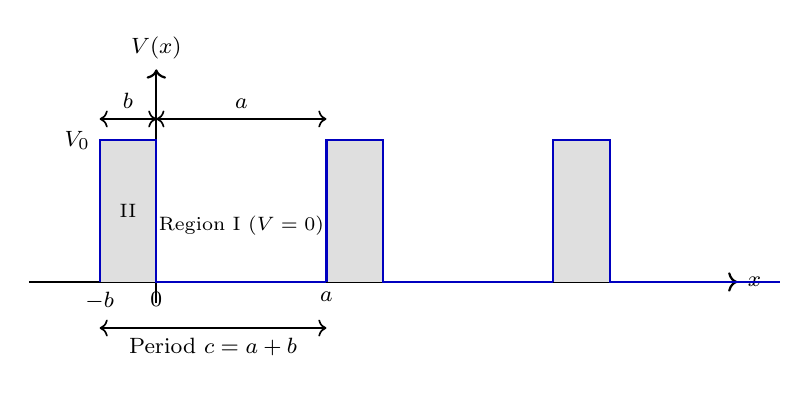
\begin{tikzpicture}[scale=0.9]
    \draw[->,thick] (-1.8,0) -- (8.2,0) node[right,font=\footnotesize] {$x$};
    \draw[->,thick] (0,-0.3) -- (0,3.0) node[above,font=\footnotesize] {$V(x)$};
    \foreach \xoff in {0,3.2,6.4}{
        \fill[gray!25] (\xoff-0.8,0) rectangle (\xoff,2.0);
        \draw[thick,blue!75!black] (\xoff-0.8,0) -- (\xoff-0.8,2.0) -- (\xoff,2.0) -- (\xoff,0) -- (\xoff+2.4,0);
    }
    \draw[<->,semithick] (-0.8,2.3) -- (0,2.3) node[midway,above,font=\footnotesize]{$b$};
    \draw[<->,semithick] (0,2.3) -- (2.4,2.3) node[midway,above,font=\footnotesize]{$a$};
    \draw[<->,semithick] (-0.8,-0.65) -- (2.4,-0.65) node[midway,below,font=\footnotesize]{Period $c = a + b$};
    \node[left,font=\footnotesize] at (-0.8,2.0) {$V_0$};
    \node[below,font=\footnotesize] at (0,0) {$0$};
    \node[below,font=\footnotesize] at (2.4,0) {$a$};
    \node[below,font=\footnotesize] at (-0.8,0) {$-b$};
    \node[font=\scriptsize] at (1.2,0.8) {Region I ($V=0$)};
    \node[font=\scriptsize] at (-0.4,1.0) {II};
\end{tikzpicture}
\caption{Periodic rectangular barrier potential $V(x)$ of the 1D Kronig--Penney model.}
\label{fig:kp_potential_master}
\end{figure}

\subsubsection{Step 1: Differential Equations in Regions I and II (Both $\psi(x)$ and $u_k(x)$ Routes)}
For sub-barrier energies $0 < E < V_0$, define the real wavevector parameters:
\begin{equation}
    \alpha \equiv \sqrt{\frac{2mE}{\hbarsq}}, \qquad \beta \equiv \sqrt{\frac{2m(V_0 - E)}{\hbarsq}}.
\end{equation}
In **Region I** ($0 < x < a$, $V=0$) and **Region II** ($-b < x < 0$, $V=V_0$), the Schr\"odinger equations for $\psi(x)$ are:
\begin{align}
    \dvtwo{\psi_{\mathrm{I}}}{x} + \alpha^2\psi_{\mathrm{I}} &= 0 \implies \psi_{\mathrm{I}}(x) = A e^{i\alpha x} + B e^{-i\alpha x}, \\
    \dvtwo{\psi_{\mathrm{II}}}{x} - \beta^2\psi_{\mathrm{II}} &= 0 \implies \psi_{\mathrm{II}}(x) = C e^{\beta x} + D e^{-\beta x}.
\end{align}
Equivalently, substituting the Bloch form $\psi(x) = e^{ikx}u_k(x)$ directly into the Schr\"odinger equation gives the differential equations for the cell-periodic function $u_k(x)$:
\begin{align}
    \dvtwo{u_1}{x} + 2ik\dv{u_1}{x} + (\alpha^2 - k^2)u_1 &= 0 \implies u_1(x) = A e^{i(\alpha-k)x} + B e^{-i(\alpha+k)x} \quad (0 < x < a), \\
    \dvtwo{u_2}{x} + 2ik\dv{u_2}{x} - (\beta^2 + k^2)u_2 &= 0 \implies u_2(x) = C e^{(\beta-ik)x} + D e^{-(\beta+ik)x} \quad (-b < x < 0).
\end{align}

\subsubsection{Step 2: Boundary Conditions and Full \texorpdfstring{$4\times 4$}{4x4} Determinant Reduction}
Continuity of $\psi$ and $\psi'$ at $x=0$, together with the Bloch periodicity condition $\psi_{\mathrm{I}}(a) = e^{ikc}\psi_{\mathrm{II}}(-b)$ and $\psi_{\mathrm{I}}'(a) = e^{ikc}\psi_{\mathrm{II}}'(-b)$ (or $u_1(a)=u_2(-b)$ and $u_1'(a)=u_2'(-b)$), yields four homogeneous linear equations for $(A, B, C, D)$:
\begin{align}
    \text{(i)}\quad \psi_{\mathrm{I}}(0) = \psi_{\mathrm{II}}(0): \qquad & A + B = C + D, \label{eq:kp_m1}\\
    \text{(ii)}\quad \psi_{\mathrm{I}}'(0) = \psi_{\mathrm{II}}'(0): \qquad & i\alpha(A - B) = \beta(C - D), \label{eq:kp_m2}\\
    \text{(iii)}\quad \psi_{\mathrm{I}}(a) = e^{ikc}\psi_{\mathrm{II}}(-b): \qquad & A e^{i\alpha a} + B e^{-i\alpha a} = e^{ikc}\left(C e^{-\beta b} + D e^{\beta b}\right), \label{eq:kp_m3}\\
    \text{(iv)}\quad \psi_{\mathrm{I}}'(a) = e^{ikc}\psi_{\mathrm{II}}'(-b): \qquad & i\alpha\left(A e^{i\alpha a} - B e^{-i\alpha a}\right) = e^{ikc}\beta\left(C e^{-\beta b} - D e^{\beta b}\right). \label{eq:kp_m4}
\end{align}
In matrix form $M\vb{v} = \vb{0}$:
\begin{equation}
    \det \begin{pmatrix}
        1 & 1 & -1 & -1 \\
        i\alpha & -i\alpha & -\beta & \beta \\
        e^{i\alpha a} & e^{-i\alpha a} & -e^{ikc}e^{-\beta b} & -e^{ikc}e^{\beta b} \\
        i\alpha e^{i\alpha a} & -i\alpha e^{-i\alpha a} & -e^{ikc}\beta e^{-\beta b} & e^{ikc}\beta e^{\beta b}
    \end{pmatrix} = 0.
\end{equation}
\textbf{Explicit Algebraic Reduction of the $4\times 4$ System:}
Define the two auxiliary combinations $S \equiv C + D$ and $M \equiv C - D$. From Eqs.~\eqref{eq:kp_m1} and \eqref{eq:kp_m2}, we express $A+B$ and $A-B$ directly in terms of $S$ and $M$:
\begin{equation}
    A + B = S, \qquad A - B = -i\frac{\beta}{\alpha}M.
\end{equation}
Now rewrite the left-hand sides of Eqs.~\eqref{eq:kp_m3} and \eqref{eq:kp_m4} using $e^{\pm i\alpha a} = \cos(\alpha a) \pm i\sin(\alpha a)$ and the right-hand sides using $e^{\pm\beta b} = \cosh(\beta b) \pm \sinh(\beta b)$:
\begin{align}
    (A+B)\cos(\alpha a) + i(A-B)\sin(\alpha a) &= e^{ikc}\big[(C+D)\cosh(\beta b) - (C-D)\sinh(\beta b)\big], \\
    i\alpha\big[(A-B)\cos(\alpha a) + i(A+B)\sin(\alpha a)\big] &= e^{ikc}\beta\big[(C-D)\cosh(\beta b) - (C+D)\sinh(\beta b)\big].
\end{align}
Substituting $A+B = S$ and $A-B = -i\frac{\beta}{\alpha}M$ (and dividing the second equation by $\beta$) collapses the $4\times 4$ system into a $2\times 2$ homogeneous system in $(S, M)$:
\begin{align}
    \big[\cos(\alpha a) - e^{ikc}\cosh(\beta b)\big]S + \left[\frac{\beta}{\alpha}\sin(\alpha a) + e^{ikc}\sinh(\beta b)\right]M &= 0, \\
    \left[-\frac{\alpha}{\beta}\sin(\alpha a) + e^{ikc}\sinh(\beta b)\right]S + \big[\cos(\alpha a) - e^{ikc}\cosh(\beta b)\big]M &= 0.
\end{align}
Setting the determinant of this $2\times 2$ matrix to zero:
\begin{equation}
    \big[\cos(\alpha a) - e^{ikc}\cosh(\beta b)\big]^2 - \left[\frac{\beta}{\alpha}\sin(\alpha a) + e^{ikc}\sinh(\beta b)\right]\left[-\frac{\alpha}{\beta}\sin(\alpha a) + e^{ikc}\sinh(\beta b)\right] = 0.
\end{equation}
Expanding both products:
\begin{equation}
    \cos^2(\alpha a) - 2e^{ikc}\cos(\alpha a)\cosh(\beta b) + e^{2ikc}\cosh^2(\beta b) + \sin^2(\alpha a) - e^{ikc}\left(\frac{\beta}{\alpha} - \frac{\alpha}{\beta}\right)\sin(\alpha a)\sinh(\beta b) - e^{2ikc}\sinh^2(\beta b) = 0.
\end{equation}
Using $\cos^2(\alpha a) + \sin^2(\alpha a) = 1$ and $\cosh^2(\beta b) - \sinh^2(\beta b) = 1$:
\begin{equation}
    1 + e^{2ikc} - 2e^{ikc}\left[\cos(\alpha a)\cosh(\beta b) + \frac{\beta^2 - \alpha^2}{2\alpha\beta}\sin(\alpha a)\sinh(\beta b)\right] = 0.
\end{equation}
Dividing by $2e^{ikc}$ and noting that $\frac{e^{-ikc} + e^{ikc}}{2} = \cos(kc) = \cos[k(a+b)]$, we obtain the **exact Kronig--Penney dispersion relation**:
\begin{equation}
    \boxed{\frac{\beta^2 - \alpha^2}{2\alpha\beta}\sinh(\beta b)\sin(\alpha a) + \cosh(\beta b)\cos(\alpha a) = \cos[k(a+b)].}
    \label{eq:kp_exact_master}
\end{equation}

\subsubsection{Step 3: The Dirac-Delta Barrier Limit (\texorpdfstring{$b \to 0, V_0 \to \infty$}{b -> 0, V_0 -> infinity})}
Taking the limit $b \to 0$ and $V_0 \to \infty$ while keeping the barrier area $V_0 b$ constant ($V(x) = V_0 b \sum_s \delta(x - sa)$), we have $c = a+b \to a$, $\beta b \to 0 \implies \sinh(\beta b) \approx \beta b$, $\cosh(\beta b) \approx 1$, and $\beta^2 - \alpha^2 \approx \beta^2 = \frac{2mV_0}{\hbarsq}$. The prefactor of $\sin(\alpha a)$ becomes:
\begin{equation}
    \frac{\beta^2 - \alpha^2}{2\alpha\beta}\sinh(\beta b) \longrightarrow \frac{\beta^2}{2\alpha\beta}(\beta b) = \frac{\beta^2 b a}{2(\alpha a)} = \left(\frac{m V_0 b a}{\hbarsq}\right)\frac{1}{\alpha a} \equiv \frac{P}{\alpha a}, \qquad \boxed{P \equiv \frac{m V_0 b a}{\hbarsq}.}
\end{equation}
Equation~\eqref{eq:kp_exact_master} simplifies to the standard **Kronig--Penney delta-comb equation**:
\begin{equation}
    \boxed{f(\alpha a) \equiv P\frac{\sin(\alpha a)}{\alpha a} + \cos(\alpha a) = \cos(ka), \qquad \alpha = \frac{\sqrt{2mE}}{\hb}.}
    \label{eq:kp_delta_master}
\end{equation}

\subsubsection{Step 4: Alternative Derivation of the KP Equation in Reciprocal Space (from the Central Equation)}
For a periodic Dirac-delta array $U(x) = A a \sum_s \delta(x - sa)$ (where $A = V_0 b / a$), every Fourier coefficient is equal:
\begin{equation}
    U_G = \frac{1}{a}\int_{-a/2}^{a/2} A a\,\delta(x) e^{-iGx}\,\dd x = A.
\end{equation}
The Central Equation~\eqref{eq:central_eq_master} becomes:
\begin{equation}
    (\lambda_k - E)C(k) + A\sum_{n=-\infty}^\infty C\left(k - \frac{2\pi n}{a}\right) = 0.
\end{equation}
Defining $F(k) \equiv \sum_n C(k - 2\pi n/a)$ and noting that $F(k - 2\pi m/a) = F(k)$, we divide by $(\lambda_{k-2\pi n/a} - E)$ and sum over all $n$:
\begin{equation}
    C\left(k - \frac{2\pi n}{a}\right) = -\frac{A F(k)}{\lambda_{k-2\pi n/a} - E} \implies 1 = -A\sum_{n=-\infty}^\infty \frac{1}{\frac{\hbarsq}{2m}\left(k - \frac{2\pi n}{a}\right)^2 - \frac{\hbarsq\alpha^2}{2m}}.
\end{equation}
Using the standard cotangent partial-fraction identity $\sum_{n=-\infty}^\infty \frac{1}{(k a - 2\pi n)^2 - (\alpha a)^2} = \frac{\sin(\alpha a)}{2\alpha a[\cos(\alpha a) - \cos(ka)]}$ gives:
\begin{equation}
    \left(\frac{m A a^2}{\hbarsq}\right)\frac{\sin(\alpha a)}{\alpha a} + \cos(\alpha a) = \cos(ka),
\end{equation}
which is identical to Eq.~\eqref{eq:kp_delta_master} with $P = \frac{m A a^2}{\hbarsq} = \frac{m V_0 b a}{\hbarsq}$.

\subsubsection{Graphical Analysis and Limiting Cases}
Because a propagating Bloch state requires a real wavevector $k$, $-1 \le \cos(ka) \le +1$:
\begin{itemize}
    \item \textbf{Allowed Energy Bands:} Ranges of $\alpha a$ where $-1 \le f(\alpha a) \le +1$ (green shaded intervals in Figure~\ref{fig:kp_plot_master}).
    \item \textbf{Forbidden Energy Gaps:} Ranges of $\alpha a$ where $\abs{f(\alpha a)} > 1$ ($k$ becomes complex $k = \frac{n\pi}{a} + i\kappa$, so wavefunctions decay exponentially and cannot propagate).
    \item \textbf{Limit 1 ($P \to 0$, Free Electron Limit):} $f(\alpha a) = \cos(\alpha a) = \cos(ka) \implies \alpha = k \implies E = \frac{\hbarsq k^2}{2m}$ (continuous parabola, all gaps vanish).
    \item \textbf{Limit 2 ($P \to \infty$, Isolated Infinite Square Wells):} Finite $f(\alpha a)$ requires $\sin(\alpha a) = 0 \implies \alpha a = n\pi \implies E_n = \frac{n^2\pi^2\hbarsq}{2ma^2}$ (bands collapse to flat, discrete atomic-like levels).
\end{itemize}

\begin{figure}[htbp]
\centering
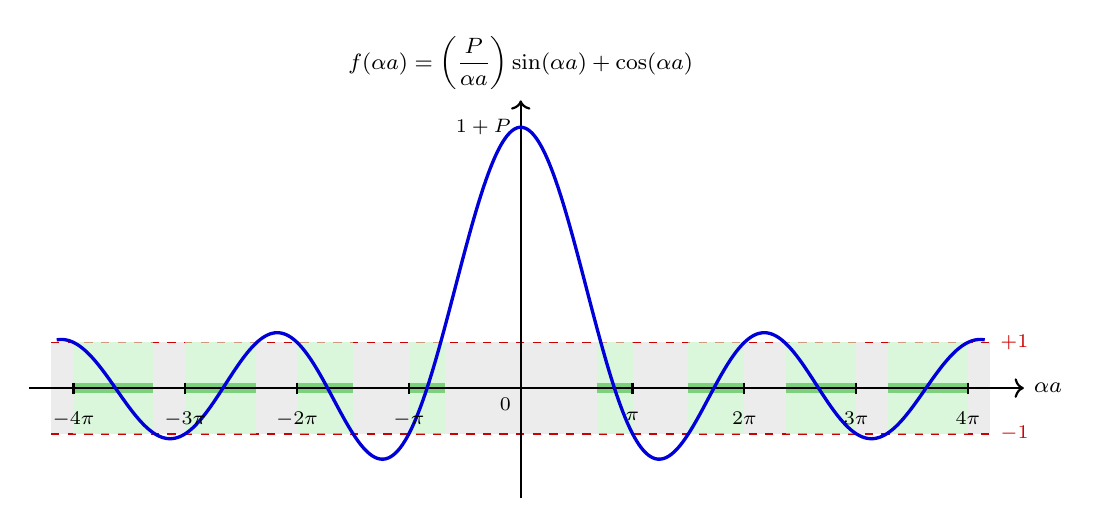
\begin{tikzpicture}[x=1.42cm, y=0.58cm]
  \fill[gray!15] (-4.2,-1) rectangle (4.2,1);
  \draw[dashed, red!80!black, semithick] (-4.2, 1) -- (4.2, 1) node[right, font=\scriptsize] {$+1$};
  \draw[dashed, red!80!black, semithick] (-4.2,-1) -- (4.2,-1) node[right, font=\scriptsize] {$-1$};

  \foreach \xa/\xb in {0.6802/1.0000, 1.4962/2.0000, 2.3693/3.0000, 3.2850/4.0000}{
    \draw[line width=3.5pt, green!55!black] ( \xa,0) -- ( \xb,0);
    \draw[line width=3.5pt, green!55!black] (-\xb,0) -- (-\xa,0);
    \fill[green!18, opacity=0.6] ( \xa,-1) rectangle ( \xb,1);
    \fill[green!18, opacity=0.6] (-\xb,-1) rectangle (-\xa,1);
  }

  \draw[->, thick] (-4.4,0) -- (4.5,0) node[right, font=\footnotesize] {$\alpha a$};
  \draw[->, thick] (0,-2.4) -- (0,6.3) node[above, font=\footnotesize] {$f(\alpha a) = \left(\dfrac{P}{\alpha a}\right)\sin(\alpha a) + \cos(\alpha a)$};

  \draw[blue!85!black, very thick, smooth]
    plot[domain=-4.15:-0.02, samples=200] (\x, {4.712389*sin(\x*180)/(\x*3.14159265) + cos(\x*180)})
    -- (0, 5.7124) --
    plot[domain=0.02:4.15, samples=200] (\x, {4.712389*sin(\x*180)/(\x*3.14159265) + cos(\x*180)});

  \foreach \n/\lab in {-4/{-4\pi}, -3/{-3\pi}, -2/{-2\pi}, -1/{-\pi}, 1/{\pi}, 2/{2\pi}, 3/{3\pi}, 4/{4\pi}}{
    \draw[thick] (\n,0.12) -- (\n,-0.12) node[below=3pt, font=\scriptsize] {$\lab$};
  }
  \node[below left, font=\scriptsize] at (0,0) {$0$};
  \node[left, font=\scriptsize] at (0,5.7124) {$1+P$};
\end{tikzpicture}
\caption{Plot of the Kronig--Penney function $f(\alpha a) = (P/\alpha a)\sin(\alpha a) + \cos(\alpha a)$ for $P = 3\pi/2$. Allowed energy bands where $\abs{f(\alpha a)} \le 1$ are highlighted in green along the $\alpha a$ axis.}
\label{fig:kp_plot_master}
\end{figure}

\begin{examplebox}{Kronig--Penney Model in the Weak-Barrier Limit ($P \ll 1$) and for $P = 10$}{ex:kp_solved}
\textbf{Problem.} (a) For $P \ll 1$, derive the lowest band energy $E(0)$ at $k=0$ and the first energy gap $E_g$ at $k = \pi/a$. (b) For $P = 10$, compute the width of the first allowed band in units of $E_\pi \equiv \frac{\pi^2\hbarsq}{2ma^2}$.
\vspace{0.2cm}\hrule\vspace{0.2cm}
\textbf{Solution.}
\textbf{(a)} At $k = 0$, $\cos(ka) = 1$ and $\alpha a \ll 1$. Expanding $\sin(\alpha a) \approx \alpha a - \frac{(\alpha a)^3}{6}$ and $\cos(\alpha a) \approx 1 - \frac{(\alpha a)^2}{2}$ in Eq.~\eqref{eq:kp_delta_master}:
\[
    P\left(1 - \frac{(\alpha a)^2}{6}\right) + 1 - \frac{(\alpha a)^2}{2} = 1 \implies (\alpha a)^2 \approx 2P \implies \frac{2mE(0)a^2}{\hbarsq} \approx 2P \implies \boxed{E(0) \approx \frac{\hbarsq P}{ma^2}.}
\]
At $k = \pi/a$, $\cos(ka) = -1$. The top of the first band sits at $\alpha_1 a = \pi$. The bottom of the second band sits at $\alpha_2 a = \pi + \delta$ ($\delta \ll 1$). Using $\sin(\pi+\delta) \approx -\delta$ and $\cos(\pi+\delta) \approx -1 + \frac{\delta^2}{2}$:
\[
    P\left(\frac{-\delta}{\pi}\right) - 1 + \frac{\delta^2}{2} = -1 \implies \delta \approx \frac{2P}{\pi} \implies E_g = \frac{\hbarsq}{2ma^2}\big[(\pi+\delta)^2 - \pi^2\big] \approx \frac{\hbarsq}{2ma^2}(2\pi\delta) = \boxed{\frac{2\hbarsq P}{ma^2}.}
\]
\textbf{(b)} For $P = 10$, the bottom of Band 1 ($f(\alpha_1 a) = +1$) satisfies $10\frac{\sin(\alpha_1 a)}{\alpha_1 a} + \cos(\alpha_1 a) = 1 \implies \alpha_1 a \approx 2.628\ \mathrm{rad}$, while the top of Band 1 ($f(\alpha_2 a) = -1$) is at $\alpha_2 a = \pi$. Thus:
\[
    \Delta E_1 = \left[1 - \left(\frac{2.628}{\pi}\right)^2\right]E_\pi = (1 - 0.700)\,E_\pi = \mathbf{0.300\,\frac{\pi^2\hbarsq}{2ma^2}}.
\]
\end{examplebox}

\subsection{The Tight-Binding (LCAO) Approximation: Complete Derivation}
Whereas the NFE model starts from delocalized plane waves, the **Tight-Binding (Linear Combination of Atomic Orbitals, LCAO) approximation** starts from localized atomic orbitals $\phi(\rvec - \RR_j)$ of isolated atoms satisfying:
\begin{equation}
    \mathcal{H}_{\mathrm{at}}(\rvec - \RR_j)\phi(\rvec - \RR_j) = E_0 \phi(\rvec - \RR_j), \qquad \mathcal{H}_{\mathrm{at}} = -\frac{\hbarsq}{2m}\nabla^2 + U_{\mathrm{at}}(\rvec - \RR_j).
\end{equation}
In the crystal, the full Hamiltonian relative to site $\RR_j$ is decomposed as:
\begin{equation}
    \mathcal{H} = \mathcal{H}_{\mathrm{at}}(\rvec - \RR_j) + \Delta U(\rvec - \RR_j), \qquad \text{where } \Delta U(\rvec - \RR_j) \equiv V(\rvec) - U_{\mathrm{at}}(\rvec - \RR_j) = \sum_{m \neq j} U_{\mathrm{at}}(\rvec - \RR_m) < 0
\end{equation}
is the perturbation potential due to all other ion cores in the crystal.

\subsubsection{Bloch Sum Ansatz and Verification of Bloch's Theorem}
We construct a trial wavefunction as a phased Bloch sum over all $N$ lattice sites:
\begin{equation}
    \psi_{\kk}(\rvec) = \frac{1}{\sqrt{N}}\sum_{j=1}^N e^{i\kk\cdot\RR_j}\phi(\rvec - \RR_j).
    \label{eq:tb_bloch_sum}
\end{equation}
\textbf{Proof that Eq.~\eqref{eq:tb_bloch_sum} satisfies Bloch's Theorem:} Under a lattice translation $\rvec \to \rvec + \RR_m$ (defining $\RR_j' \equiv \RR_j - \RR_m$):
\begin{equation}
    \psi_{\kk}(\rvec + \RR_m) = \frac{1}{\sqrt{N}}\sum_{j=1}^N e^{i\kk\cdot\RR_j}\phi\big(\rvec - (\RR_j - \RR_m)\big) = e^{i\kk\cdot\RR_m}\frac{1}{\sqrt{N}}\sum_{j'=1}^N e^{i\kk\cdot\RR_j'}\phi(\rvec - \RR_j') = e^{i\kk\cdot\RR_m}\psi_{\kk}(\rvec). \quad \checkmark
\end{equation}

\subsubsection{Evaluation of the First-Order Energy Expectation Value}
Assuming orbitals on distinct sites are approximately orthonormal ($\braket{\phi_m}{\phi_j} \approx \delta_{mj}$, so $\braket{\psi_{\kk}}{\psi_{\kk}} \approx 1$), the energy expectation value is:
\begin{align}
    E(\kk) &= \mel{\psi_{\kk}}{\mathcal{H}}{\psi_{\kk}} = \frac{1}{N}\sum_{j=1}^N \sum_{m=1}^N e^{i\kk\cdot(\RR_j - \RR_m)} \int \phi^*(\rvec - \RR_m)\big[E_0 + \Delta U(\rvec - \RR_j)\big]\phi(\rvec - \RR_j)\,\dd^3 r.
\end{align}
Setting $\boldsymbol{\rho}_m \equiv \RR_m - \RR_j$ and shifting integration variables to $\rvec' = \rvec - \RR_j$, the sum over $j$ gives $N$ identical copies cancelling the $\frac{1}{N}$ prefactor:
\begin{equation}
    E(\kk) = E_0 + \sum_{\boldsymbol{\rho}_m} e^{-i\kk\cdot\boldsymbol{\rho}_m} \int \phi^*(\rvec' - \boldsymbol{\rho}_m)\Delta U(\rvec')\phi(\rvec')\,\dd^3 r'.
\end{equation}
Because atomic wavefunctions decay exponentially with distance, we retain only the **on-site crystal-field integral** ($\boldsymbol{\rho}_m = \vb{0}$) and the **nearest-neighbor overlap/hopping integrals** ($\boldsymbol{\rho}_m = \boldsymbol{\rho}$):
\begin{align}
    -\alpha_{\mathrm{TB}} &\equiv \int \abs{\phi(\rvec)}^2 \Delta U(\rvec)\,\dd^3 r < 0 \qquad (\text{on-site energy shift; define } \epsilon_0 \equiv E_0 - \alpha_{\mathrm{TB}}), \\
    -\gamma \equiv -\beta_{\mathrm{TB}} \equiv t &\equiv \int \phi^*(\rvec - \boldsymbol{\rho})\Delta U(\rvec)\phi(\rvec)\,\dd^3 r \qquad (\text{nearest-neighbor hopping integral, } \gamma > 0 \text{ for } s\text{-orbitals}).
\end{align}
This yields the general nearest-neighbor tight-binding dispersion relation:
\begin{equation}
    \boxed{E(\kk) = E_0 - \alpha_{\mathrm{TB}} - \gamma\sum_{\boldsymbol{\rho}\in\mathrm{NN}} e^{-i\kk\cdot\boldsymbol{\rho}} = \epsilon_0 - \gamma\sum_{\boldsymbol{\rho}\in\mathrm{NN}} e^{-i\kk\cdot\boldsymbol{\rho}}.}
    \label{eq:tb_general_master}
\end{equation}

\subsubsection{Explicit Tight-Binding Dispersions for 1D, 2D, and 3D Crystal Lattices}
\begin{enumerate}
    \item \textbf{1D Chain ($2$ nearest neighbors at $\rho = \pm a$):}
    \begin{equation}
        \boxed{E(k) = \epsilon_0 - \gamma(e^{-ika} + e^{ika}) = \epsilon_0 - 2\gamma\cos(ka), \qquad \text{Bandwidth } W = E_{\max} - E_{\min} = 4\gamma.}
    \end{equation}
    \item \textbf{2D Square Lattice ($4$ nearest neighbors at $(\pm a, 0), (0, \pm a)$):}
    \begin{equation}
        \boxed{E(\kk) = \epsilon_0 - 2\gamma\big[\cos(k_x a) + \cos(k_y a)\big], \qquad \text{Bandwidth } W = 8\gamma.}
    \end{equation}
    \item \textbf{3D Simple Cubic (SC) Lattice ($6$ nearest neighbors at $(\pm a,0,0),(0,\pm a,0),(0,0,\pm a)$):}
    \begin{equation}
        \boxed{E(\kk) = \epsilon_0 - 2\gamma\big[\cos(k_x a) + \cos(k_y a) + \cos(k_z a)\big], \qquad \text{Bandwidth } W = 12\gamma.}
    \end{equation}
    \item \textbf{3D Body-Centered Cubic (BCC) Lattice ($8$ nearest neighbors at $(\pm\frac{a}{2}, \pm\frac{a}{2}, \pm\frac{a}{2})$):}
    \begin{equation}
        \boxed{E(\kk) = \epsilon_0 - 8\gamma\cos\left(\frac{k_x a}{2}\right)\cos\left(\frac{k_y a}{2}\right)\cos\left(\frac{k_z a}{2}\right), \qquad \text{Bandwidth } W = 16\gamma.}
    \end{equation}
    \item \textbf{3D Face-Centered Cubic (FCC) Lattice ($12$ nearest neighbors at $(\pm\frac{a}{2}, \pm\frac{a}{2}, 0)$, etc.):}
    \begin{equation}
        \boxed{E(\kk) = \epsilon_0 - 4\gamma\left[\cos\left(\frac{k_x a}{2}\right)\cos\left(\frac{k_y a}{2}\right) + \cos\left(\frac{k_y a}{2}\right)\cos\left(\frac{k_z a}{2}\right) + \cos\left(\frac{k_z a}{2}\right)\cos\left(\frac{k_x a}{2}\right)\right], \quad W = 16\gamma.}
    \end{equation}
\end{enumerate}

\begin{figure}[htbp]
\centering
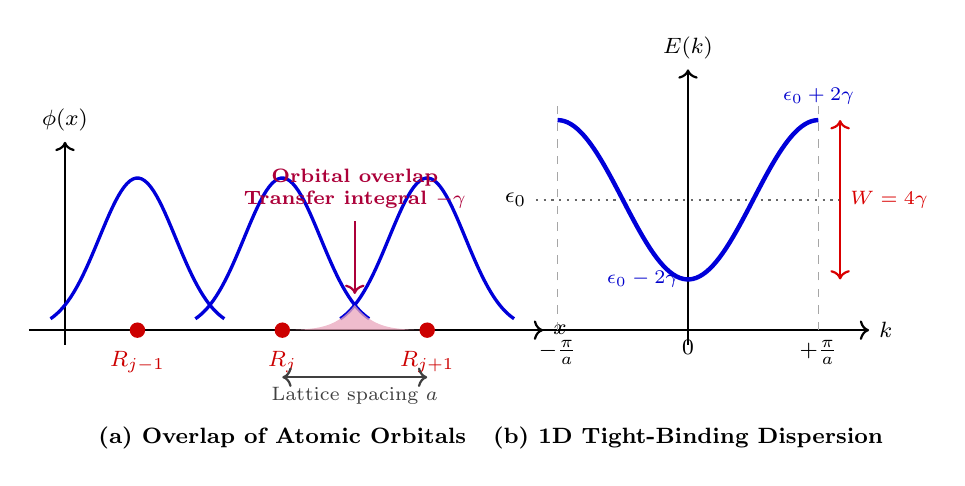
\begin{tikzpicture}[scale=0.92]
  % (a) Atomic Orbital Overlap
  \begin{scope}[shift={(0,0)}]
    \draw[->,thick] (-0.5,0) -- (6.6,0) node[right,font=\footnotesize] {$x$};
    \draw[->,thick] (0,-0.2) -- (0,2.6) node[above,font=\footnotesize] {$\phi(x)$};
    
    % Three atomic centers: R_{j-1}=1.0, R_j=3.0, R_{j+1}=5.0
    \draw[blue!85!black,very thick] plot[domain=-0.2:2.2,samples=60] (\x, {2.1*exp(-1.8*(\x-1.0)^2)});
    \draw[blue!85!black,very thick] plot[domain=1.8:4.2,samples=60] (\x, {2.1*exp(-1.8*(\x-3.0)^2)});
    \draw[blue!85!black,very thick] plot[domain=3.8:6.2,samples=60] (\x, {2.1*exp(-1.8*(\x-5.0)^2)});
    
    % Shaded overlap region between R_j (3.0) and R_{j+1} (5.0)
    \fill[purple!35,opacity=0.75] 
      plot[domain=3.0:4.0,samples=35] (\x, {2.1*exp(-1.8*(\x-5.0)^2)}) --
      plot[domain=4.0:5.0,samples=35] (\x, {2.1*exp(-1.8*(\x-3.0)^2)}) --
      (5.0,0) -- (3.0,0) -- cycle;
      
    % Atom cores
    \filldraw[red!80!black] (1.0,0) circle (2.8pt) node[below=4pt,font=\footnotesize\bfseries] {$R_{j-1}$};
    \filldraw[red!80!black] (3.0,0) circle (2.8pt) node[below=4pt,font=\footnotesize\bfseries] {$R_j$};
    \filldraw[red!80!black] (5.0,0) circle (2.8pt) node[below=4pt,font=\footnotesize\bfseries] {$R_{j+1}$};
    
    % Lattice spacing a
    \draw[<->,thick,darkgray] (3.0,-0.65) -- (5.0,-0.65) node[midway,below,font=\scriptsize] {Lattice spacing $a$};
    
    % Overlap annotation
    \draw[->,thick,purple!90!black] (4.0,1.5) -- (4.0,0.5);
    \node[above,font=\scriptsize\bfseries,align=center,purple!90!black] at (4.0,1.55) {Orbital overlap\\Transfer integral $-\gamma$};
    
    \node[below,font=\footnotesize\bfseries] at (3.0,-1.2) {(a) Overlap of Atomic Orbitals};
  \end{scope}

  % (b) 1D Tight-Binding Dispersion
  \begin{scope}[shift={(8.6,0)}]
    \draw[->,thick] (-2.5,0) -- (2.5,0) node[right,font=\footnotesize] {$k$};
    \draw[->,thick] (0,-0.2) -- (0,3.6) node[above,font=\footnotesize] {$E(k)$};
    
    % Brillouin zone boundaries
    \draw[dashed,gray!70] (-1.8,0) -- (-1.8,3.2);
    \draw[dashed,gray!70] (1.8,0) -- (1.8,3.2);
    \node[below,font=\footnotesize] at (-1.8,0) {$-\frac{\pi}{a}$};
    \node[below,font=\footnotesize] at (0,0) {$0$};
    \node[below,font=\footnotesize] at (1.8,0) {$+\frac{\pi}{a}$};
    
    % Atomic level epsilon_0
    \draw[dotted,thick,gray!80!black] (-2.1,1.8) -- (2.1,1.8);
    \node[left,font=\footnotesize] at (-2.1,1.8) {$\epsilon_0$};
    
    % Dispersion curve E(k) = \epsilon_0 - 2\gamma\cos(ka)
    \draw[ultra thick,blue!85!black] plot[domain=-1.8:1.8,samples=80] (\x, {1.8 - 1.1*cos(\x*180/1.8)});
    
    % Band edges
    \node[left,font=\scriptsize,blue!80!black] at (0,0.7) {$\epsilon_0 - 2\gamma$};
    \node[above=2pt,font=\scriptsize,blue!80!black] at (1.8,2.9) {$\epsilon_0 + 2\gamma$};
    
    % Bandwidth W = 4\gamma
    \draw[<->,thick,red!85!black] (2.1,0.7) -- (2.1,2.9) node[midway,right,font=\scriptsize\bfseries] {$W = 4\gamma$};
    
    \node[below,font=\footnotesize\bfseries] at (0,-1.2) {(b) 1D Tight-Binding Dispersion};
  \end{scope}
\end{tikzpicture}
\caption{(a) Spatial overlap of neighboring atomic orbitals $\phi(x - R_j)$ and $\phi(x - R_{j+1})$ giving rise to the hopping transfer integral $-\gamma$; (b) resulting 1D tight-binding energy band $E(k) = \epsilon_0 - 2\gamma\cos(ka)$ of total bandwidth $W = 4\gamma$.}
\label{fig:tb_model_master}
\end{figure}

\begin{examplebox}{1D Tight-Binding Density of States and van Hove Singularities}{ex:tb_dos_master}
\textbf{Problem.} Derive the exact electronic density of states per unit length (including spin) for the 1D tight-binding band $E(k) = \epsilon_0 - 2\gamma\cos(ka)$, and evaluate $D(E)$ at the band center $E = \epsilon_0$ for $\gamma = 1.0\ \mathrm{eV}$ and $a = 2.0\ \text{\AA}$.
\vspace{0.2cm}\hrule\vspace{0.2cm}
\textbf{Solution.}
Including $g_s = 2$ spins and both $+k$ and $-k$ branches in $[-\pi/a, \pi/a]$, the number of states per unit length in $\dd E$ is $D(E)\,\dd E = 2 \times 2 \times \frac{\dd k}{2\pi} = \frac{2}{\pi}\abs{\dv{E}{k}}^{-1}\dd E$. Differentiating $E(k)$:
\[
    \abs{\dv{E}{k}} = 2\gamma a\abs{\sin(ka)} = 2\gamma a\sqrt{1 - \cos^2(ka)} = 2\gamma a\sqrt{1 - \left(\frac{E - \epsilon_0}{2\gamma}\right)^2} = a\sqrt{4\gamma^2 - (E - \epsilon_0)^2}.
\]
Substituting this into $D(E)$ yields:
\[
    \boxed{D(E) = \frac{2}{\pi a\sqrt{4\gamma^2 - (E - \epsilon_0)^2}}, \qquad (\epsilon_0 - 2\gamma < E < \epsilon_0 + 2\gamma).}
\]
At the band edges $E \to \epsilon_0 \pm 2\gamma$ (where $v_g = 0$), $D(E)$ diverges as $\abs{E - E_{\mathrm{edge}}}^{-1/2}$ (**1D van Hove singularities**). At $E = \epsilon_0$, $D(\epsilon_0) = \frac{1}{\pi a\gamma} = \frac{1}{\pi(2.0\times 10^{-10}\ \mathrm{m})(1.0\ \mathrm{eV})} = \mathbf{1.59 \times 10^{9}\ \mathrm{m^{-1}\,eV^{-1}}}$.
\end{examplebox}

% ============================================================================
\section{Motion of Electrons in Bands, Effective Mass, Holes, and Bloch Oscillations}
\label{sec:electron_dynamics}
% ============================================================================

\subsection{The Semiclassical Paradigm and Criteria for Validity}
A single stationary Bloch state $\psi_{n\kk}(\rvec) = e^{i\kk\cdot\rvec}u_{n\kk}(\rvec)$ has probability density $\abs{\psi_{n\kk}(\rvec)}^2 = \abs{u_{n\kk}(\rvec)}^2$, which is periodic across the entire crystal ($\Delta x \to \infty$). To describe a spatially localized electron moving under external macroscopic electric and magnetic fields ($\bm{\mathcal{E}}, \vb{B}$), we form a **wave packet** from Bloch states within a single band $n$ centered around wavevector $\kk_0$:
\begin{equation}
    \Psi_n(\rvec, t) = \int_{\BZ} A(\kk)\,\psi_{n\kk}(\rvec)\exp\left[-\frac{iE_n(\kk)t}{\hb}\right]\dd^3 k,
\end{equation}
where $A(\kk)$ is sharply peaked within $\Delta k$ around $\kk_0$ (Figure~\ref{fig:wavepacket_master}).

\begin{figure}[htbp]
\centering
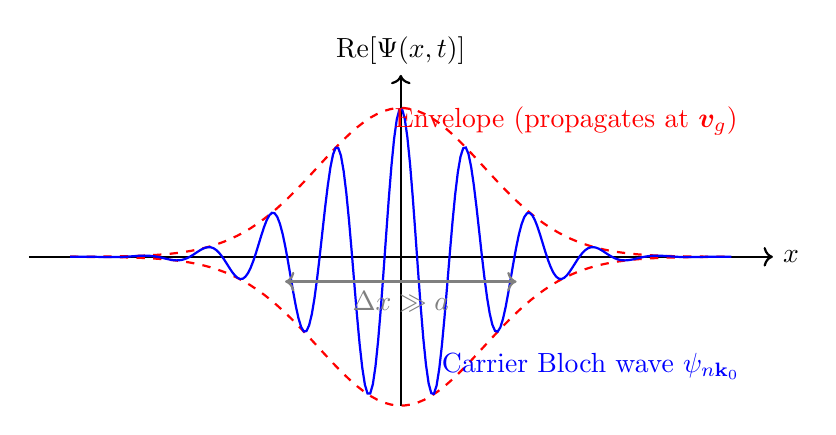
\begin{tikzpicture}[scale=1.05]
    \draw[->, thick] (-4.5,0) -- (4.5,0) node[right] {$x$};
    \draw[->, thick] (0,-1.8) -- (0,2.2) node[above] {$\text{Re}[\Psi(x,t)]$};
    \draw[dashed, red, thick, domain=-4:4, samples=100] plot (\x, {1.8*exp(-\x*\x/2)});
    \draw[dashed, red, thick, domain=-4:4, samples=100] plot (\x, {-1.8*exp(-\x*\x/2)});
    \draw[blue, thick, domain=-4:4, samples=250] plot (\x, {1.8*exp(-\x*\x/2)*cos(8*\x r)});
    \node[red, above] at (2.0, 1.35) {Envelope (propagates at $\bm{v}_g$)};
    \node[blue, below] at (2.3, -1.05) {Carrier Bloch wave $\psi_{n\kk_0}$};
    \draw[<->, gray, thick] (-1.4,-0.3) -- (1.4,-0.3);
    \node[gray, below] at (0,-0.3) {$\Delta x \gg a$};
\end{tikzpicture}
\caption{Localized Bloch electron wave packet in a crystal: the high-frequency carrier is the Bloch function, while the Gaussian envelope propagates at the group velocity $\bm{v}_g = \hb^{-1}\nabla_{\kk}E(\kk)$.}
\label{fig:wavepacket_master}
\end{figure}

\paragraph{Three Criteria for Semiclassical Validity (Absence of Interband Transitions):}
\begin{enumerate}
    \item \textbf{Spatial Scale Separation:} The wave-packet width $\Delta x$ must be much larger than the lattice constant $a$ (so $\Delta k \sim 1/\Delta x \ll \pi/a$ is well-localized in the Brillouin zone), yet much smaller than the variation wavelength $L_{\mathrm{ext}}$ of the applied fields:
    \begin{equation}
        a \ll \Delta x \ll L_{\mathrm{ext}}.
    \end{equation}
    \item \textbf{No Zener Breakdown (Electric Field Limit):} The electrostatic energy gained across one lattice spacing must be much smaller than the band gap $E_g$:
    \begin{equation}
        e\abs{\bm{\mathcal{E}}}a \ll E_g \qquad \left(\text{typically } \abs{\bm{\mathcal{E}}} \ll \frac{E_g}{ea} \sim 10^8\text{--}10^9\ \mathrm{V/m}\right).
    \end{equation}
    \item \textbf{Magnetic and Frequency Limits:} $\hb\omega_c \ll E_g$ (no magnetic breakdown) and $\hb\omega \ll E_g$ (no direct optical interband absorption).
\end{enumerate}

\subsection{Two Complete Derivations of the Group Velocity \texorpdfstring{$\vb{v}_g = \frac{1}{\hb}\nabla_{\kk}E_n(\kk)$}{v_g = (1/hbar) grad_k E_n(k)}}

\subsubsection{Derivation 1: Wave-Packet Envelope and Stationary Phase}
Expanding $E_n(\kk)$ in a first-order Taylor series around $\kk_0$:
\begin{equation}
    E_n(\kk) \approx E_n(\kk_0) + (\kk - \kk_0)\cdot\big[\nabla_{\kk}E_n(\kk)\big]_{\kk_0},
\end{equation}
and approximating $u_{n\kk}(\rvec) \approx u_{n\kk_0}(\rvec)$ across the narrow range $\Delta k$, the wave packet becomes:
\begin{equation}
    \Psi_n(\rvec, t) \approx \psi_{n\kk_0}(\rvec) e^{-iE_n(\kk_0)t/\hb} \underbrace{\int_{\BZ} A(\kk)\exp\left\{i(\kk-\kk_0)\cdot\left[\rvec - \left(\frac{1}{\hb}\nabla_{\kk}E_n(\kk)\right)t\right]\right\}\dd^3 k}_{\equiv\, \Phi(\rvec - \vb{v}_g t)}.
\end{equation}
Because the envelope $\Phi(\rvec - \vb{v}_g t)$ depends on $\rvec$ and $t$ exclusively through the combination $\rvec - \vb{v}_g t$, the center of probability of the wave packet travels at the **group velocity**:
\begin{equation}
    \boxed{\vb{v}_g(\kk) = \nabla_{\kk}\omega(\kk) = \frac{1}{\hb}\nabla_{\kk}E_n(\kk).}
    \label{eq:vg_master}
\end{equation}

\subsubsection{Derivation 2: Exact Quantum Expectation Value via the Hellmann--Feynman Theorem}
We now prove rigorously that the quantum mechanical expectation value of the velocity operator $\hat{\vb{v}} = \frac{\hat{\vb{p}}}{m} = -\frac{i\hb}{m}\nabla$ in a stationary Bloch state $\psi_{n\kk}(\rvec)$ equals $\frac{1}{\hb}\nabla_{\kk}E_n(\kk)$.
Recall that $u_{n\kk}(\rvec) = e^{-i\kk\cdot\rvec}\psi_{n\kk}(\rvec)$ satisfies the $\kk$-shifted eigenvalue equation:
\begin{equation}
    \hat{H}_{\kk} u_{n\kk}(\rvec) = E_n(\kk) u_{n\kk}(\rvec), \qquad \text{where } \hat{H}_{\kk} \equiv e^{-i\kk\cdot\rvec}\hat{H}_0 e^{i\kk\cdot\rvec} = \frac{1}{2m}(-i\hb\nabla + \hb\kk)^2 + V(\rvec).
\end{equation}
Differentiating the operator $\hat{H}_{\kk}$ with respect to $\kk$:
\begin{equation}
    \nabla_{\kk}\hat{H}_{\kk} = \frac{\hb}{m}(-i\hb\nabla + \hb\kk) = \hb\,e^{-i\kk\cdot\rvec}\left(\frac{\hat{\vb{p}}}{m}\right)e^{i\kk\cdot\rvec} = \hb\,e^{-i\kk\cdot\rvec}\hat{\vb{v}}\,e^{i\kk\cdot\rvec}.
\end{equation}
By the **Hellmann--Feynman theorem**, $\nabla_{\kk}E_n(\kk) = \mel{u_{n\kk}}{\nabla_{\kk}\hat{H}_{\kk}}{u_{n\kk}}$. Therefore:
\begin{equation}
    \nabla_{\kk}E_n(\kk) = \hb\mel{u_{n\kk}}{e^{-i\kk\cdot\rvec}\hat{\vb{v}}\,e^{i\kk\cdot\rvec}}{u_{n\kk}} = \hb\mel{\psi_{n\kk}}{\hat{\vb{v}}}{\psi_{n\kk}} \implies \boxed{\expect{\hat{\vb{v}}}_{n\kk} = \frac{1}{\hb}\nabla_{\kk}E_n(\kk) = \vb{v}_g(\kk).} \quad \blacksquare
\end{equation}

\subsection{Semiclassical Equation of Motion and Crystal Momentum}
Suppose an electron wave packet is subjected to an external electric field $\bm{\mathcal{E}}$, exerting force $\vb{F}_{\mathrm{ext}} = -e\bm{\mathcal{E}}$. Over a time interval $\dd t$, the wave packet moves by $\dd\rvec = \vb{v}_g\,\dd t$, and the external field performs mechanical work $\delta W = \vb{F}_{\mathrm{ext}}\cdot\dd\rvec = \vb{F}_{\mathrm{ext}}\cdot\vb{v}_g\,\dd t$. Since the periodic lattice potential is static and already absorbed into $E_n(\kk)$, energy conservation requires $\dd E_n(\kk) = \delta W$:
\begin{equation}
    \dd E_n(\kk) = \nabla_{\kk}E_n(\kk)\cdot\dd\kk = \hb\vb{v}_g\cdot\dd\kk = \vb{F}_{\mathrm{ext}}\cdot\vb{v}_g\,\dd t \implies \vb{v}_g\cdot\left(\hb\dv{\kk}{t} - \vb{F}_{\mathrm{ext}}\right) = 0.
\end{equation}
Including the magnetic Lorentz force $-e(\vb{v}_g\times\vb{B})$ (which acts perpendicular to $\vb{v}_g$ and does zero work), we obtain the fundamental **semiclassical equation of motion**:
\begin{equation}
    \boxed{\hb\dv{\kk}{t} = \vb{F}_{\mathrm{ext}} = -e\left(\bm{\mathcal{E}} + \vb{v}_g\times\vb{B}\right).}
    \label{eq:semiclassical_eom_master}
\end{equation}

\begin{pitfallbox}{Crystal Momentum $\hb\kk$ vs.\ True Mechanical Momentum $\expect{\hat{\vb{p}}} = m_0\vb{v}_g$}
A Bloch state $\psi_{n\kk}(\rvec)$ is an eigenstate of the discrete lattice translation operator $\hat{T}_{\RR}$, \textbf{not} of the momentum operator $\hat{\vb{p}} = -i\hb\nabla$:
\begin{equation}
    \hat{\vb{p}}\psi_{n\kk}(\rvec) = \hb\kk\psi_{n\kk}(\rvec) + e^{i\kk\cdot\rvec}\big(-i\hb\nabla u_{n\kk}(\rvec)\big).
\end{equation}
While $\hb\dv{\kk}{t} = \vb{F}_{\mathrm{ext}}$ depends \emph{only} on the external force, the rate of change of the electron's true mechanical momentum $m_0\dv{\vb{v}_g}{t}$ includes the internal forces exerted by the periodic ion lattice:
\begin{equation}
    m_0\dv{\vb{v}_g}{t} = \vb{F}_{\mathrm{ext}} + \vb{F}_{\mathrm{lattice}}.
\end{equation}
\end{pitfallbox}

\subsection{Acceleration and the Effective Mass Tensor: Complete Derivation and Anisotropy}

\subsubsection{Motivation: Absorbing the Internal Lattice Potential}
In classical Newtonian mechanics, the acceleration of an electron subjected to an external electric field $\bm{\mathcal{E}}$ is governed by the total force:
\begin{equation}
    m_0 \dv{\vb{v}}{t} = \vb{F}_{\mathrm{total}} = \vb{F}_{\mathrm{ext}} + \vb{F}_{\mathrm{lattice}},
\end{equation}
where $\vb{F}_{\mathrm{ext}} = -e\bm{\mathcal{E}}$ is the macroscopic applied force, and $\vb{F}_{\mathrm{lattice}} = -\nabla V(\rvec)$ is the microscopic electrostatic Coulomb force exerted by the $\sim 10^{23}\ \mathrm{cm^{-3}}$ atomic ion cores. The lattice force fluctuates violently over sub-angstrom distances with field intensities of $\sim 10^{11}\ \mathrm{V/m}$, rendering direct solution intractable for macroscopic electron transport.

The foundational paradigm of the semiclassical model is that the crystal lattice potential is \emph{already completely absorbed} into the energy dispersion relation $E_n(\kk)$. Consequently, we seek an equation of motion relating the wave packet's acceleration $\vb{a} \equiv \dv{\vb{v}_g}{t}$ \emph{directly to the external force alone}:
\begin{equation}
    \vb{a} = (\vb{m}^*)^{-1} \vb{F}_{\mathrm{ext}},
\end{equation}
where all the quantum interactions with the periodic ion cores are encapsulated in the dynamic parameter known as the \textbf{effective mass tensor} $\vb{m}^*$.

\subsubsection{Complete Step-by-Step Derivation of the Acceleration}
The $i$-th Cartesian component of the wave packet group velocity is given by Eq.~\eqref{eq:vg_master}:
\begin{equation}
    v_{g,i}(\kk) = \frac{1}{\hb}\frac{\partial E(\kk)}{\partial k_i}, \qquad (i = x, y, z).
\end{equation}
To determine the wave packet acceleration $a_i = \dv{v_{g,i}}{t}$, we differentiate with respect to time $t$:
\begin{equation}
    a_i = \dv{}{t}\left(\frac{1}{\hb}\frac{\partial E(\kk)}{\partial k_i}\right).
\end{equation}
Because the wavevector $\kk(t) = \big(k_x(t), k_y(t), k_z(t)\big)$ evolves continuously in time under the external force, we apply the multivariable chain rule over all three reciprocal-space coordinates:
\begin{align}
    a_i &= \frac{1}{\hb} \sum_{j=x,y,z} \frac{\partial}{\partial k_j}\left(\frac{\partial E(\kk)}{\partial k_i}\right) \dv{k_j}{t} \nonumber \\
        &= \frac{1}{\hb} \sum_{j=x,y,z} \frac{\partial^2 E(\kk)}{\partial k_i \partial k_j} \dv{k_j}{t}.
        \label{eq:ai_chain_rule}
\end{align}
Next, we invoke the fundamental semiclassical equation of motion, Eq.~\eqref{eq:semiclassical_eom_master}:
\begin{equation}
    \hb\dv{\kk}{t} = \vb{F}_{\mathrm{ext}} \implies \dv{k_j}{t} = \frac{1}{\hb} F_{\mathrm{ext},j}.
\end{equation}
Substituting this rate of change into Eq.~\eqref{eq:ai_chain_rule}:
\begin{equation}
    a_i = \frac{1}{\hb} \sum_{j=x,y,z} \frac{\partial^2 E(\kk)}{\partial k_i \partial k_j} \left(\frac{1}{\hb} F_{\mathrm{ext},j}\right) = \sum_{j=x,y,z} \left(\frac{1}{\hbarsq}\frac{\partial^2 E(\kk)}{\partial k_i \partial k_j}\right) F_{\mathrm{ext},j}.
\end{equation}
Comparing this relation directly with the tensor formulation of Newton's second law:
\begin{equation}
    a_i = \sum_{j=x,y,z} \left(\frac{1}{m^*}\right)_{ij} F_{\mathrm{ext},j},
\end{equation}
we obtain the exact mathematical definition of the components of the \textbf{inverse effective mass tensor}:
\begin{equation}
    \boxed{\left(\frac{1}{m^*}\right)_{ij} = \frac{1}{\hbarsq}\frac{\partial^2 E(\kk)}{\partial k_i \partial k_j}.}
    \label{eq:mstar_tensor_master}
\end{equation}
In compact dyadic matrix notation, this reads:
\begin{equation}
    \vb{a} = (\vb{m}^*)^{-1}\vb{F}_{\mathrm{ext}} \iff \vb{F}_{\mathrm{ext}} = \vb{m}^*\vb{a}.
\end{equation}

\subsubsection{Tensor Symmetry, Diagonalization, and Non-Collinear Acceleration}
By Schwarz's theorem on the equality of mixed partial derivatives (since $E(\kk)$ is twice continuously differentiable across the Brillouin zone):
\begin{equation}
    \frac{\partial^2 E(\kk)}{\partial k_i \partial k_j} = \frac{\partial^2 E(\kk)}{\partial k_j \partial k_i} \implies \left(\frac{1}{m^*}\right)_{ij} = \left(\frac{1}{m^*}\right)_{ji}.
\end{equation}
The inverse effective mass tensor is therefore a real, symmetric second-rank tensor (represented by a $3\times 3$ symmetric matrix). 

From linear algebra, any real symmetric tensor can be diagonalized by performing an orthogonal coordinate rotation to its \textbf{principal crystallographic axes}:
\begin{equation}
    (\vb{m}^{*-1})_{\mathrm{diag}} = \begin{pmatrix}
        \frac{1}{m_{xx}^*} & 0 & 0 \\
        0 & \frac{1}{m_{yy}^*} & 0 \\
        0 & 0 & \frac{1}{m_{zz}^*}
    \end{pmatrix}.
\end{equation}
In this principal coordinate system, the acceleration components decouple:
\begin{equation}
    a_x = \frac{F_{\mathrm{ext},x}}{m_{xx}^*}, \qquad a_y = \frac{F_{\mathrm{ext},y}}{m_{yy}^*}, \qquad a_z = \frac{F_{\mathrm{ext},z}}{m_{zz}^*}.
\end{equation}

\begin{takeawaybox}{Profound Physical Consequence: Non-Collinear Acceleration}
In free space, $\vb{a} = \vb{F}/m_0$ is always strictly parallel to $\vb{F}$. In a crystal lattice with anisotropic band curvature ($m_{xx}^* \neq m_{yy}^* \neq m_{zz}^*$), \textbf{the acceleration vector $\vb{a}$ is generally not parallel to the applied force $\vb{F}_{\mathrm{ext}}$!} 

For example, if an electric field is applied at an angle $\theta$ in the $xy$-plane ($F_x = F\cos\theta, F_y = F\sin\theta$), the ratio of accelerations is:
\begin{equation}
    \tan\theta_a = \frac{a_y}{a_x} = \left(\frac{m_{xx}^*}{m_{yy}^*}\right)\tan\theta.
\end{equation}
If $m_{xx}^* > m_{yy}^*$, then $\tan\theta_a > \tan\theta$: the electron is deflected sideways towards the direction of lighter effective mass!
\end{takeawaybox}

\subsubsection{Ellipsoidal Valleys in Real Crystals: Longitudinal and Transverse Mass}
In cubic semiconductors like Silicon ($\text{Si}$) and Germanium ($\text{Ge}$), the conduction band minima do not reside at $\kk = \vb{0}$, but rather at equivalent off-center valleys. In Silicon, there are $M_c = 6$ equivalent minima along the $\langle 100 \rangle$ directions in reciprocal space. 

Near the minimum along the $[001]$ direction ($k_{0z} \approx 0.85\frac{2\pi}{a}$), the constant-energy surfaces are ellipsoids of revolution described by:
\begin{equation}
    E(\kk) = E_c + \frac{\hbarsq}{2}\left[\frac{k_x^2 + k_y^2}{m_t^*} + \frac{(k_z - k_{0z})^2}{m_l^*}\right],
    \label{eq:ellipsoidal_valleys}
\end{equation}
where:
\begin{itemize}[noitemsep]
    \item $m_l^*$ is the \textbf{longitudinal effective mass} measured along the valley major axis (along $[001]$): for $\text{Si}$, $m_l^* \approx 0.98\,m_0$.
    \item $m_t^*$ is the \textbf{transverse effective mass} measured perpendicular to the valley axis (in the $xy$-plane): for $\text{Si}$, $m_t^* \approx 0.19\,m_0$.
\end{itemize}

Because electrons in transport populate all $6$ valleys simultaneously, we must carefully distinguish two different macroscopic averages:
\begin{enumerate}
    \item \textbf{Density-of-States Effective Mass ($m_{de}^*$):} The number of available states per unit volume per unit energy depends on the volume enclosed by the constant energy ellipsoids:
    \begin{equation}
        m_{de}^* = M_c^{2/3}\big(m_l^* m_t^{*2}\big)^{1/3} = 6^{2/3}\big(0.98 \times 0.19^2\big)^{1/3}m_0 \approx \mathbf{1.08\,m_0}.
    \end{equation}
    This is the mass that enters the effective density of states $N_c = 2\left(\frac{2\pi m_{de}^* k_B T}{h^2}\right)^{3/2}$.
    \item \textbf{Conductivity (Transport) Effective Mass ($m_{\sigma}^*$):} For an electric field applied along an arbitrary direction in cubic Silicon, two valleys have longitudinal mass along the field, and four valleys have transverse mass. The isotropic average inverse mass is:
    \begin{equation}
        \frac{1}{m_{\sigma}^*} = \frac{1}{3}\left(\frac{1}{m_l^*} + \frac{2}{m_t^*}\right) \implies m_{\sigma}^* = \frac{3 m_l^* m_t^*}{2m_l^* + m_t^*} = \frac{3(0.98)(0.19)}{2(0.98) + 0.19}m_0 \approx \mathbf{0.26\,m_0}.
    \end{equation}
    This is the mass that determines the electron drift mobility $\mu_e = \frac{e\tau}{m_{\sigma}^*}$ and electrical conductivity $\sigma = n e \mu_e$.
\end{enumerate}

\subsubsection{Parabolic Band Approximation and Band Curvature}
For an isotropic, spherically symmetric band or in a one-dimensional crystal, the effective mass tensor reduces to a single scalar:
\begin{equation}
    a = \frac{1}{\hbarsq}\dvtwo{E}{k} F_{\mathrm{ext}} \implies \boxed{m^*(k) = \frac{\hbarsq}{\dvtwo{E}{k}}.}
    \label{eq:mstar_scalar_master}
\end{equation}
Taylor expanding the energy $E(k)$ around a band minimum ($k=0$):
\begin{equation}
    E(k) = E(0) + \left.\dv{E}{k}\right|_0 k + \frac{1}{2}\left.\dvtwo{E}{k}\right|_0 k^2 + \mathcal{O}(k^3).
\end{equation}
Because $k=0$ is an extremum, $\left.\dv{E}{k}\right|_0 = 0$. Truncating at second order gives the **parabolic band approximation**:
\begin{equation}
    E(k) \approx E_c + \frac{\hbarsq k^2}{2m^*}, \qquad \text{where } m^* = \frac{\hbarsq}{\left.\dvtwo{E}{k}\right|_0}.
\end{equation}
\begin{itemize}
    \item \textbf{Sharp, High Curvature ($\dvtwo{E}{k} \gg 0$):} Results in an exceptionally \textbf{small effective mass} $m^* \ll m_0$. Examples include $\text{InSb}$ ($m_e^* = 0.014\,m_0$) and $\text{GaAs}$ ($m_e^* = 0.067\,m_0$). Under small electric fields, electrons experience enormous accelerations, yielding high drift mobilities ($\mu_e \sim 10^4\text{--}10^5\ \mathrm{cm^2/(V\cdot s)}$).
    \item \textbf{Broad, Flat Band ($\dvtwo{E}{k} \approx 0$):} Results in a \textbf{large effective mass} $m^* \gg m_0$. Typical of transition-metal $d$-bands or the heavy-hole valence band ($m_{hh}^* \approx 0.5\,m_0$). Electrons are sluggish and exhibit low drift mobilities.
\end{itemize}

\subsection{Detailed Analysis of a 1D Tight-Binding Band, Negative Effective Mass, and Bragg Reaction Force}

\subsubsection{Mathematical Framework for a 1D Band}
To explore the variation of group velocity and effective mass across the entire Brillouin zone, consider a 1D crystal with lattice constant $a$, on-site energy $E_0$, and nearest-neighbor hopping matrix element $t > 0$:
\begin{equation}
    E(k) = E_0 - 2t\cos(ka).
\end{equation}
The total bandwidth is $W = E(\pi/a) - E(0) = 4t$. Taking the first and second derivatives with respect to wavevector $k$:
\begin{align}
    v_g(k) &= \frac{1}{\hb}\dv{E}{k} = \frac{2ta}{\hb}\sin(ka), \label{eq:tb_vg} \\
    \dvtwo{E}{k} &= 2ta^2\cos(ka) \implies \frac{1}{m^*(k)} = \frac{2ta^2}{\hbarsq}\cos(ka), \label{eq:tb_curv} \\
    m^*(k) &= \frac{\hbarsq}{2ta^2\cos(ka)}. \label{eq:tb_mstar}
\end{align}

\subsubsection{Exhaustive Physical Breakdown of the Three Regimes}
As plotted in Figure~\ref{fig:effmass_panels_master}, the first Brillouin zone $[-\pi/a, +\pi/a]$ partitions cleanly into three distinct dynamical regimes:
\begin{enumerate}
    \item \textbf{Regime 1: Band Bottom ($\abs{k} < \frac{\pi}{2a}$):}
    Here $\cos(ka) > 0$, meaning the band has upward curvature ($\dvtwo{E}{k} > 0$), and the effective mass is strictly positive:
    \begin{equation}
        m^*(k) > 0.
    \end{equation}
    Near $k=0$, expanding $\cos(ka) \approx 1 - \frac{1}{2}(ka)^2$:
    \begin{equation}
        E(k) \approx (E_0 - 2t) + ta^2k^2 = E_{\min} + \frac{\hbarsq k^2}{2m^*(0)}, \qquad \text{with } m^*(0) = +\frac{\hbarsq}{2ta^2}.
    \end{equation}
    The electron behaves as an ordinary free particle with a renormalized positive mass. Acceleration is collinear with the external force: $\vb{a} = \vb{F}_{\mathrm{ext}}/m^*(0)$.

    \item \textbf{Regime 2: Inflection Points ($k = \pm\frac{\pi}{2a}$):}
    At $k = \pm\frac{\pi}{2a}$, $\cos(ka) = 0$, so the band curvature vanishes:
    \begin{equation}
        \dvtwo{E}{k} = 0 \implies \frac{1}{m^*} = 0 \implies m^* \to \pm\infty.
    \end{equation}
    Simultaneously, the group velocity reaches its global maximum:
    \begin{equation}
        v_{\max} = \frac{2ta}{\hb}.
    \end{equation}
    Here, an applied external force produces \textbf{zero acceleration}:
    \begin{equation}
        a = \frac{F_{\mathrm{ext}}}{m^*} \to 0.
    \end{equation}
    The electron propagates at its maximum possible velocity and does not speed up, regardless of field intensity.

    \item \textbf{Regime 3: Band Top ($\frac{\pi}{2a} < \abs{k} \le \frac{\pi}{a}$):}
    Here $\cos(ka) < 0$, meaning the band curves downwards ($\dvtwo{E}{k} < 0$), yielding a strictly \textbf{negative effective mass}:
    \begin{equation}
        m^*(k) < 0.
    \end{equation}
    Near the zone boundary $k \to \pm\frac{\pi}{a}$, let $q = k \mp \frac{\pi}{a}$. Then $\cos(ka) = -\cos(qa) \approx -(1 - \frac{1}{2}q^2a^2)$:
    \begin{equation}
        E(k) \approx (E_0 + 2t) - ta^2q^2 = E_{\max} - \frac{\hbarsq q^2}{2\abs{m^*(\pi/a)}}, \qquad \text{with } m^*(\pm\pi/a) = -\frac{\hbarsq}{2ta^2}.
    \end{equation}
    Under a positive forward force $F_{\mathrm{ext}} > 0$, the wave packet experiences negative acceleration ($a < 0$): \textbf{it decelerates!}
\end{enumerate}

\begin{table}[htbp]
\centering
\small
\renewcommand{\arraystretch}{1.25}
\begin{tabular}{lcccc}
\toprule
\textbf{Wavevector $k$} & \textbf{Band Curvature $\dvtwo{E}{k}$} & \textbf{Group Velocity $v_g$} & \textbf{Effective Mass $m^*(k)$} & \textbf{Physical Dynamical Behavior} \\
\midrule
$k = 0$ (Zone center) & $+2ta^2$ (maximum $>0$) & $0$ & $+\frac{\hbarsq}{2ta^2} > 0$ & Accelerates forward like normal particle \\
$0 < \abs{k} < \frac{\pi}{2a}$ & Positive ($>0$) & Increasing ($>0$) & Positive ($>0$) & Speeds up in direction of external force \\
$k = \pm\frac{\pi}{2a}$ (Inflection) & $0$ & $\pm v_{\max} = \pm \frac{2ta}{\hb}$ & $\pm\infty$ & Zero acceleration ($a=0$); maximal velocity \\
$\frac{\pi}{2a} < \abs{k} < \frac{\pi}{a}$ & Negative ($<0$) & Decreasing & Negative ($<0$) & Decelerates while moving forward \\
$k = \pm\frac{\pi}{a}$ (Zone boundary) & $-2ta^2$ (minimum $<0$) & $0$ & $-\frac{\hbarsq}{2ta^2} < 0$ & Standing wave; Bragg backscattering \\
\bottomrule
\end{tabular}
\caption{Comprehensive dynamical behavior of an electron in a 1D tight-binding band across the first Brillouin zone.}
\label{tab:1d_regimes_summary}
\end{table}

\subsubsection{Microscopic Mechanism of Negative Effective Mass: Bragg Reaction Forces}
The concept of a negative mass appears contradictory if one forgets the periodic crystal lattice. The paradox is resolved by examining the true momentum balance equation:
\begin{equation}
    m_0 a = F_{\mathrm{total}} = F_{\mathrm{ext}} + F_{\mathrm{lattice}},
\end{equation}
where $m_0$ is the invariant positive rest mass of the free electron, and $F_{\mathrm{lattice}} = -\expect{\nabla V(\rvec)}$ is the total electrostatic force exerted on the electron by the periodic ions.

Substituting the semiclassical operational definition of acceleration, $a = F_{\mathrm{ext}}/m^*$:
\begin{equation}
    m_0\left(\frac{F_{\mathrm{ext}}}{m^*}\right) = F_{\mathrm{ext}} + F_{\mathrm{lattice}}.
\end{equation}
Solving for the force exerted by the crystal lattice yields the exact relation:
\begin{equation}
    \boxed{F_{\mathrm{lattice}} = \left(\frac{m_0}{m^*} - 1\right)F_{\mathrm{ext}}.}
    \label{eq:flattice_master}
\end{equation}
Equation~\eqref{eq:flattice_master} reveals the physical origin of the three regimes:
\begin{itemize}
    \item When $m^* = m_0$, $F_{\mathrm{lattice}} = 0$: the electron moves without net force from the lattice (free electron limit).
    \item When $0 < m^* < m_0$, $\left(\frac{m_0}{m^*} - 1\right) > 0 \implies F_{\mathrm{lattice}}$ is positive. The periodic lattice exerts a force in the \emph{same direction} as $F_{\mathrm{ext}}$, assisting the acceleration so the electron acts lighter than in vacuum.
    \item When $m^* \to \infty$, $F_{\mathrm{lattice}} = -F_{\mathrm{ext}}$: the periodic ions pull backwards with equal magnitude, exactly canceling the external field ($F_{\mathrm{total}} = 0 \implies a = 0$).
    \item When $m^* < 0$, the factor $\frac{m_0}{m^*}$ is negative, which guarantees:
    \begin{equation}
        \left(\frac{m_0}{m^*} - 1\right) < -1 \implies \abs{F_{\mathrm{lattice}}} > \abs{F_{\mathrm{ext}}}.
    \end{equation}
    The backward force exerted by the periodic lattice on the electron is \textbf{strictly greater in magnitude than the applied forward force!}
\end{itemize}

\paragraph{Why does the lattice pull backwards near the zone boundary?}
As the forward force $F_{\mathrm{ext}} > 0$ accelerates the electron, $k$ increases towards the Brillouin zone boundary $\pi/a$. The electron's de Broglie wavelength $\lambda = \frac{2\pi}{k}$ shrinks towards $\lambda = 2a$. 

This precisely satisfies the Bragg diffraction condition $2a\sin 90^\circ = \lambda$ for constructive backscattering from successive lattice planes. The forward-traveling wave packet is strongly reflected into a backward-traveling wave. Each coherent reflection transfers a discrete packet of reciprocal lattice momentum $\hb G = \frac{2\pi\hb}{a}$ to the crystal lattice. 

By Newton's third law, the recoiling crystal lattice exerts an equal and opposite backward reaction force on the electron. In the upper half of the band ($\abs{k} > \frac{\pi}{2a}$), the rate of momentum transfer from Bragg backscattering exceeds the rate of momentum input from the external field:
\begin{equation}
    F_{\mathrm{total}} = F_{\mathrm{ext}} + F_{\mathrm{lattice}} < 0.
\end{equation}
The electron decelerates ($a < 0$) because the \emph{net physical force} acting on it is directed backwards! Because the semiclassical equation assigns all acceleration to $F_{\mathrm{ext}}$ via $a = F_{\mathrm{ext}}/m^*$, the backward net acceleration forces $m^*$ to be mathematically negative. The effective mass is not a property of the electron itself, but an envelope parameter absorbing the quantum mechanical momentum exchange with the crystal lattice.

\subsubsection{Band-Edge Effective Mass from the Nearly Free Electron (NFE) Model}
We can also derive the band-edge effective mass from the Nearly Free Electron model developed in Section 2. Near the zone boundary $k = \frac{\pi}{a} + q$, degenerate perturbation theory yielded the two split band energies, Eq.~\eqref{eq:nfe_general_dispersion}:
\begin{equation}
    E_\pm(q) = \frac{\hbarsq}{2m_0}\left[\left(\frac{\pi}{a}\right)^2 + q^2\right] \pm \sqrt{\left(\frac{\hbarsq \pi q}{m_0 a}\right)^2 + \abs{V_G}^2}.
\end{equation}
Defining the zone-boundary kinetic energy $E_{\BZ} \equiv \frac{\hbarsq(\pi/a)^2}{2m_0}$ and expanding the square root for small $q$ ($q \ll \frac{m_0 a \abs{V_G}}{\hb^2 \pi}$):
\begin{equation}
    \sqrt{\abs{V_G}^2 + \left(\frac{\hbarsq \pi q}{m_0 a}\right)^2} \approx \abs{V_G}\left[1 + \frac{1}{2}\left(\frac{\hbarsq \pi q}{m_0 a \abs{V_G}}\right)^2\right] = \abs{V_G} + \frac{\hbarsq q^2}{2m_0}\left(\frac{2E_{\BZ}}{\abs{V_G}}\right).
\end{equation}
Substituting this into $E_\pm(q)$ gives the parabolic dispersion near the gap edges:
\begin{equation}
    E_\pm(q) \approx \big(E_{\BZ} \pm \abs{V_G}\big) + \frac{\hbarsq q^2}{2m_0}\left(1 \pm \frac{2E_{\BZ}}{\abs{V_G}}\right).
\end{equation}
Differentiating twice with respect to $q$ yields the **NFE band-edge effective mass formula**:
\begin{equation}
    \boxed{\frac{1}{m_\pm^*} = \frac{1}{\hbarsq}\dvtwo{E_\pm}{q} = \frac{1}{m_0}\left(1 \pm \frac{2E_{\BZ}}{\abs{V_G}}\right) = \frac{1}{m_0}\left(1 \pm \frac{4E_{\BZ}}{E_g}\right).}
    \label{eq:nfe_mstar_formula_detailed}
\end{equation}
Because the periodic lattice potential is weak in the NFE approximation ($\abs{V_G} \ll E_{\BZ}$), the second term overwhelmingly dominates ($\frac{4E_{\BZ}}{E_g} \gg 1$):
\begin{itemize}
    \item \textbf{Lower Band (Valence Band Edge $E_-$):}
    \begin{equation}
        \frac{1}{m_-^*} \approx -\frac{1}{m_0}\frac{4E_{\BZ}}{E_g} < 0 \implies m_-^* \approx -\left(\frac{E_g}{4E_{\BZ}}\right)m_0 < 0.
    \end{equation}
    The valence band maximum has sharp negative curvature, producing a negative effective mass.
    \item \textbf{Upper Band (Conduction Band Edge $E_+$):}
    \begin{equation}
        \frac{1}{m_+^*} \approx +\frac{1}{m_0}\frac{4E_{\BZ}}{E_g} > 0 \implies m_+^* \approx +\left(\frac{E_g}{4E_{\BZ}}\right)m_0 > 0.
    \end{equation}
    The conduction band minimum has sharp positive curvature, producing a light positive effective mass.
\end{itemize}
\begin{takeawaybox}{Band Gap Scaling of Effective Mass}
Equation~\eqref{eq:nfe_mstar_formula_detailed} reveals that the band-edge effective mass is \textbf{directly proportional to the forbidden energy gap}: $m^* \propto E_g$. When the band gap is narrow, the level repulsion between the two zone-boundary states induces extreme curvature, creating extraordinarily lightweight, high-mobility electrons and holes. This rigorously explains why narrow-gap semiconductors such as $\text{InSb}$ ($E_g = 0.17\ \mathrm{eV}, m_e^* = 0.014\,m_0$) have electron effective masses nearly two orders of magnitude smaller than wide-gap semiconductors such as $\text{GaN}$ ($E_g = 3.4\ \mathrm{eV}, m_e^* = 0.20\,m_0$).
\end{takeawaybox}

\begin{figure}[htbp]
\centering
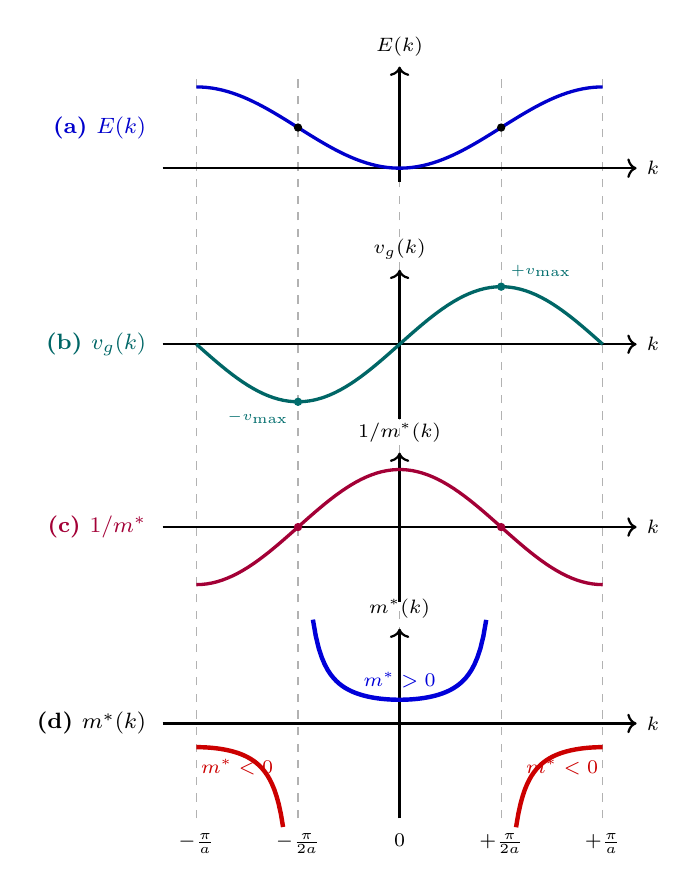
\begin{tikzpicture}[scale=0.86]
    \foreach \x in {-3.0, -1.5, 0, 1.5, 3.0}{
        \draw[dashed,gray!60] (\x,-8.8) -- (\x,2.2);
    }
    \begin{scope}[shift={(0,0.8)}]
        \draw[->,thick] (-3.5,0) -- (3.5,0) node[right,font=\scriptsize] {$k$};
        \draw[->,thick] (0,-0.2) -- (0,1.5) node[above,font=\scriptsize] {$E(k)$};
        \draw[very thick,blue!80!black] plot[domain=-3.0:3.0,samples=80] (\x,{0.6*(1 - cos(\x*180/3.0))});
        \filldraw[black] (-1.5,0.6) circle (1.5pt);
        \filldraw[black] (1.5,0.6) circle (1.5pt);
        \node[left,font=\footnotesize\bfseries,blue!80!black] at (-3.6,0.6) {(a) $E(k)$};
    \end{scope}
    \begin{scope}[shift={(0,-1.8)}]
        \draw[->,thick] (-3.5,0) -- (3.5,0) node[right,font=\scriptsize] {$k$};
        \draw[->,thick] (0,-1.1) -- (0,1.1) node[above,font=\scriptsize] {$v_g(k)$};
        \draw[very thick,teal!80!black] plot[domain=-3.0:3.0,samples=80] (\x,{0.85*sin(\x*180/3.0)});
        \filldraw[teal!85!black] (1.5,0.85) circle (1.5pt) node[above right,font=\tiny] {$+v_{\max}$};
        \filldraw[teal!85!black] (-1.5,-0.85) circle (1.5pt) node[below left,font=\tiny] {$-v_{\max}$};
        \node[left,font=\footnotesize\bfseries,teal!80!black] at (-3.6,0) {(b) $v_g(k)$};
    \end{scope}
    \begin{scope}[shift={(0,-4.5)}]
        \draw[->,thick] (-3.5,0) -- (3.5,0) node[right,font=\scriptsize] {$k$};
        \draw[->,thick] (0,-1.1) -- (0,1.1) node[above,font=\scriptsize] {$1/m^*(k)$};
        \draw[very thick,purple!85!black] plot[domain=-3.0:3.0,samples=80] (\x,{0.85*cos(\x*180/3.0)});
        \filldraw[purple!85!black] (1.5,0) circle (1.5pt);
        \filldraw[purple!85!black] (-1.5,0) circle (1.5pt);
        \node[left,font=\footnotesize\bfseries,purple!85!black] at (-3.6,0) {(c) $1/m^*$};
    \end{scope}
    \begin{scope}[shift={(0,-7.4)}]
        \draw[->,thick] (-3.5,0) -- (3.5,0) node[right,font=\scriptsize] {$k$};
        \draw[->,thick] (0,-1.4) -- (0,1.4) node[above,font=\scriptsize] {$m^*(k)$};
        \draw[ultra thick,blue!85!black] plot[domain=-1.28:1.28,samples=60] (\x,{0.35/cos(\x*180/3.0)});
        \draw[ultra thick,red!80!black] plot[domain=-3.0:-1.72,samples=40] (\x,{0.35/cos(\x*180/3.0)});
        \draw[ultra thick,red!80!black] plot[domain=1.72:3.0,samples=40] (\x,{0.35/cos(\x*180/3.0)});
        \node[left,font=\footnotesize\bfseries,black] at (-3.6,0) {(d) $m^*(k)$};
        \node[below=2pt,font=\scriptsize] at (-3.0,-1.4) {$-\frac{\pi}{a}$};
        \node[below=2pt,font=\scriptsize] at (-1.5,-1.4) {$-\frac{\pi}{2a}$};
        \node[below=2pt,font=\scriptsize] at (0,-1.4) {$0$};
        \node[below=2pt,font=\scriptsize] at (1.5,-1.4) {$+\frac{\pi}{2a}$};
        \node[below=2pt,font=\scriptsize] at (3.0,-1.4) {$+\frac{\pi}{a}$};
        \node[font=\scriptsize\bfseries,blue!85!black,above] at (0,0.38) {$m^* > 0$};
        \node[font=\scriptsize\bfseries,red!80!black,below] at (2.4,-0.38) {$m^* < 0$};
        \node[font=\scriptsize\bfseries,red!80!black,below] at (-2.4,-0.38) {$m^* < 0$};
    \end{scope}
\end{tikzpicture}
\caption{Variation of (a) $E(k)$, (b) group velocity $v_g(k)$, (c) inverse effective mass $1/m^*(k)$, and (d) effective mass $m^*(k)$ across the first Brillouin zone $[-\pi/a, +\pi/a]$.}
\label{fig:effmass_panels_master}
\end{figure}

\subsection{\texorpdfstring{$\kk\cdot\vb{p}$}{k.p} Perturbation Theory and the Effective Mass Sum Rule \texorpdfstring{{\normalfont\normalsize\color{purple!75!black}\textbf{[Enrichment / Out of Syllabus]}}}{[Enrichment / Out of Syllabus]}}

\begin{enrichmentbox}{Course Syllabus Note}
\textbf{Syllabus Scope:} This section covers second-order $\kk\cdot\vb{p}$ perturbation theory beyond the core PH7302 examination syllabus. It is included here for students interested in advanced semiconductor optoelectronics, quantum wells, and preparation for national entrance tests (GATE / CSIR-NET / JEST).
\end{enrichmentbox}

Writing $\hat{H}_{\kk} = \hat{H}_0 + \frac{\hb}{m}\kk\cdot\hat{\vb{p}} + \frac{\hbarsq k^2}{2m}$ for the cell-periodic function $u_{n\kk}(\rvec)$ and treating $\hat{H}' = \frac{\hb}{m}\kk\cdot\hat{\vb{p}}$ to second order in perturbation theory around a band extremum at $\kk=\vb{0}$ gives:
\begin{equation}
    E_n(\kk) = E_n(\vb{0}) + \frac{\hbarsq k^2}{2m} + \frac{\hbarsq}{m^2}\sum_{j \neq n}\frac{\abs{\mel{u_{n0}}{\kk\cdot\hat{\vb{p}}}{u_{j0}}}^2}{E_n(\vb{0}) - E_j(\vb{0})}.
\end{equation}
Differentiating twice with respect to $k$ yields the **$\kk\cdot\vb{p}$ effective mass sum rule**:
\begin{equation}
    \boxed{\frac{m}{m_n^*} = 1 + \frac{2}{m}\sum_{j \neq n}\frac{\abs{\mel{u_{n0}}{\hat{p}}{u_{j0}}}^2}{E_n(\vb{0}) - E_j(\vb{0})} \approx 1 + \frac{2\abs{p_{cv}}^2}{m E_g} \quad (\text{conduction band of a direct-gap semiconductor}).}
    \label{eq:kp_sum_rule_master}
\end{equation}

\subsection{Bloch Oscillations in Clean Lattices and Semiconductor Superlattices \texorpdfstring{{\normalfont\normalsize\color{purple!75!black}\textbf{[Enrichment / Out of Syllabus]}}}{[Enrichment / Out of Syllabus]}}

\begin{enrichmentbox}{Course Syllabus Note}
\textbf{Syllabus Scope:} Coherent Bloch oscillations in ideal lattices and engineered semiconductor superlattices represent advanced dynamics beyond the core syllabus. It illustrates the stunning wave-mechanical consequence of periodic band structures under strong electric fields.
\end{enrichmentbox}

Consider a collisionless electron ($\tau \to \infty$) in a 1D tight-binding band $E(k) = E_0 - 2t\cos(ka)$ subjected to a uniform DC electric field $\mathcal{E}$ along $+x$:
\begin{equation}
    \hb\dv{k}{t} = -e\mathcal{E} \implies k(t) = k(0) - \frac{e\mathcal{E}}{\hb}t.
\end{equation}
Setting $k(0) = 0$, the group velocity and real-space position oscillate sinusoidally in time (**Bloch Oscillations**, Figure~\ref{fig:bloch_osc_master}):
\begin{align}
    v_g(t) &= \frac{2ta}{\hb}\sin\big(k(t)a\big) = -\frac{2ta}{\hb}\sin(\omega_B t), \\
    x(t) - x(0) &= \int_0^t v_g(t')\,\dd t' = \frac{2t}{e\mathcal{E}}\big[\cos(\omega_B t) - 1\big],
\end{align}
with characteristic **Bloch frequency**, **Bloch period**, and **real-space amplitude**:
\begin{equation}
    \boxed{\omega_B = \frac{e\mathcal{E}a}{\hb}, \qquad T_B = \frac{2\pi}{\omega_B} = \frac{h}{e\mathcal{E}a}, \qquad L_B = \frac{4t}{e\mathcal{E}} = \frac{W}{e\mathcal{E}}.}
\end{equation}
\textbf{Why Bloch Oscillations Are Not Observed in Bulk Metals:} For $a \approx 3\ \text{\AA}$ and $\mathcal{E} \sim 10^3\ \mathrm{V/m}$, $T_B \approx 1.4 \times 10^{-8}\ \mathrm{s}$, whereas the room-temperature scattering time is $\tau \sim 10^{-14}\ \mathrm{s} \ll T_B$. However, in artificial **$\text{GaAs}/\text{AlGaAs}$ semiconductor superlattices** with period $d \sim 10\text{--}20\ \mathrm{nm}$ and high fields, $T_B$ drops into the sub-picosecond regime ($T_B < \tau$), enabling experimental observation of terahertz Bloch oscillations.

\begin{figure}[htbp]
\centering
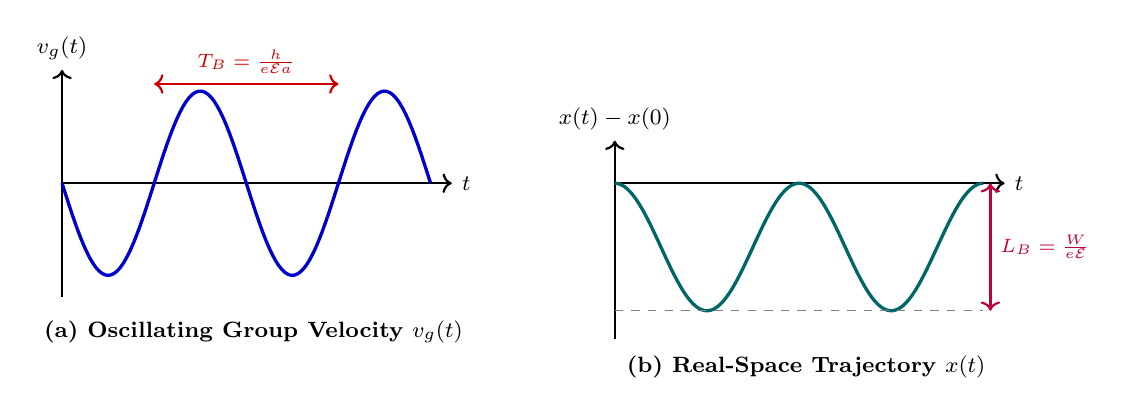
\begin{tikzpicture}[scale=0.9]
  \begin{scope}[shift={(0,0)}]
    \draw[->,thick] (0,0) -- (5.5,0) node[right,font=\footnotesize] {$t$};
    \draw[->,thick] (0,-1.6) -- (0,1.6) node[above,font=\footnotesize] {$v_g(t)$};
    \draw[very thick,blue!80!black,domain=0:5.2,samples=120] plot (\x, {-1.3*sin(\x*180/1.3)});
    \draw[<->,thick,red!80!black] (1.3,1.4) -- (3.9,1.4) node[midway,above,font=\scriptsize] {$T_B = \frac{h}{e\mathcal{E}a}$};
    \node[below,font=\footnotesize\bfseries] at (2.7,-1.8) {(a) Oscillating Group Velocity $v_g(t)$};
  \end{scope}
  \begin{scope}[shift={(7.8,0)}]
    \draw[->,thick] (0,0) -- (5.5,0) node[right,font=\footnotesize] {$t$};
    \draw[->,thick] (0,-2.2) -- (0,0.6) node[above,font=\footnotesize] {$x(t) - x(0)$};
    \draw[very thick,teal!80!black,domain=0:5.2,samples=120] plot (\x, {0.9*(cos(\x*180/1.3) - 1)});
    \draw[dashed,gray] (0,-1.8) -- (5.2,-1.8);
    \draw[<->,thick,purple] (5.3,0) -- (5.3,-1.8) node[midway,right,font=\scriptsize] {$L_B = \frac{W}{e\mathcal{E}}$};
    \node[below,font=\footnotesize\bfseries] at (2.7,-2.3) {(b) Real-Space Trajectory $x(t)$};
  \end{scope}
\end{tikzpicture}
\caption{Bloch oscillations of an electron in a periodic band under a constant DC electric field $\mathcal{E}$: (a) group velocity $v_g(t)$ and (b) bounded real-space oscillation of amplitude $L_B = W/(e\mathcal{E})$.}
\label{fig:bloch_osc_master}
\end{figure}

\subsection{Complete Electrodynamics of Holes in Nearly Filled Bands \texorpdfstring{{\normalfont\normalsize\color{purple!75!black}\textbf{[Enrichment / Out of Syllabus]}}}{[Enrichment / Out of Syllabus]}}

\begin{enrichmentbox}{Course Syllabus Note}
\textbf{Syllabus Scope:} The formal many-body transformation of an electron vacancy in an almost-filled valence band into a positive hole quasiparticle is provided here as an advanced theoretical foundation supporting the semiconductor physics in Section 5.
\end{enrichmentbox}

\begin{enumerate}
    \item \textbf{Zero Current in a Completely Filled Band:} Since $E(-\kk) = E(\kk)$, the group velocity is odd: $\vb{v}_g(-\kk) = -\vb{v}_g(\kk)$. Summing over all occupied states in a full Brillouin zone pairs every $+\kk$ with $-\kk$:
    \begin{equation}
        \vb{j}_{\mathrm{full}} = (-e)\sum_{\kk\in\BZ}\vb{v}_g(\kk) = \vb{0}, \qquad \sum_{\kk\in\BZ}\kk = \vb{0}.
    \end{equation}
    \item \textbf{Current of a Band with One Missing Electron at $\kk_e$:}
    \begin{equation}
        \vb{j} = (-e)\sum_{\kk\neq\kk_e}\vb{v}_e(\kk) = (-e)\left[\sum_{\text{all }\kk}\vb{v}_e(\kk) - \vb{v}_e(\kk_e)\right] = (+e)\vb{v}_e(\kk_e).
    \end{equation}
    Thus, the collective current of all $2N-1$ remaining electrons is identical to that of a single particle of **positive charge $+e$** moving with velocity $\vb{v}_h = \vb{v}_e(\kk_e)$ (**hole quasiparticle**).
\end{enumerate}

\begin{table}[htbp]
\centering
\renewcommand{\arraystretch}{1.2}
\begin{tabular}{lcc}
\toprule
\textbf{Physical Property} & \textbf{Missing Valence Electron State} & \textbf{Equivalent Hole Quasiparticle} \\
\midrule
Electric Charge & $-e$ & $+e$ \\
Crystal Wavevector & $\kk_e$ & $\kk_h = -\kk_e$ \\
Excitation Energy (relative to $E_v=0$) & $E_e(\kk_e) < 0$ & $E_h(\kk_h) = -E_e(\kk_e) > 0$ \\
Group Velocity & $\vb{v}_e = \hb^{-1}\nabla_{\kk_e}E_e(\kk_e)$ & $\vb{v}_h = \hb^{-1}\nabla_{\kk_h}E_h(\kk_h) = \vb{v}_e(\kk_e)$ \\
Effective Mass (near valence band top) & $m_e^* < 0$ & $m_h^* = -m_e^* > 0$ \\
Semiclassical Equation of Motion & $\hb\dot{\kk}_e = -e(\bm{\mathcal{E}} + \vb{v}_e\times\vb{B})$ & $\hb\dot{\kk}_h = +e(\bm{\mathcal{E}} + \vb{v}_h\times\vb{B})$ \\
Electrical Current Density Contribution & $-e\vb{v}_e$ & $+e\vb{v}_h$ \\
\bottomrule
\end{tabular}
\caption{Exact mathematical correspondence between a missing valence electron and a hole quasiparticle.}
\label{tab:hole_mapping_master}
\end{table}

\subsection{Motion in a Uniform Magnetic Field and Cyclotron Resonance \texorpdfstring{{\normalfont\normalsize\color{purple!75!black}\textbf{[Enrichment / Out of Syllabus]}}}{[Enrichment / Out of Syllabus]}}

\begin{enrichmentbox}{Course Syllabus Note}
\textbf{Syllabus Scope:} Magnetic orbit quantization in reciprocal space and cyclotron resonance experiments represent an enrichment topic demonstrating how band curvatures and effective masses are directly measured in experimental solid-state physics.
\end{enrichmentbox}

Under a static magnetic field $\vb{B}$ with $\bm{\mathcal{E}} = \vb{0}$, the equation of motion $\hb\dv{\kk}{t} = -e(\vb{v}_g\times\vb{B}) = -\frac{e}{\hb}(\nabla_{\kk}E \times \vb{B})$ conserves both the electron energy $E(\kk) = \text{const}$ and the wavevector component $k_\parallel$ parallel to $\vb{B}$. Thus, the electron traces out the intersection of a constant-energy surface with a plane perpendicular to $\vb{B}$. Integrating around a closed $\kk$-space orbit enclosing cross-sectional area $A(E, k_\parallel)$ gives the **cyclotron period** and **cyclotron effective mass**:
\begin{equation}
    T_c = \oint \dd t = \frac{\hbarsq}{eB}\oint \frac{\dd k_\perp}{\abs{\nabla_{\kk,\perp}E}} = \frac{\hbarsq}{eB}\frac{\partial A}{\partial E} \implies \boxed{\omega_c = \frac{eB}{m_c^*}, \qquad m_c^* = \frac{\hbarsq}{2\pi}\frac{\partial A}{\partial E}.}
\end{equation}

\begin{examplebox}{NFE Band-Edge Effective Masses and GaAs $\kk\cdot\vb{p}$ Matrix Element}{ex:effmass_solved}
\textbf{Problem.} (a) A 1D crystal with $a = 4.0\ \text{\AA}$ has a zone-boundary band gap $E_g = 2\abs{U} = 0.60\ \mathrm{eV}$ at $k = \pi/a$. Calculate the band-edge effective masses $m_+^*/m_e$ and $m_-^*/m_e$. (b) In $\text{GaAs}$ ($E_g = 1.42\ \mathrm{eV}$, $m_e^* = 0.067\,m_e$, $m_h^* = 0.50\,m_e$), calculate the Kane momentum matrix element $\abs{p_{cv}}$ and compare the electron and hole drift mobilities.
\vspace{0.2cm}\hrule\vspace{0.2cm}
\textbf{Solution.}
\textbf{(a)} At $k = \frac{\pi}{4.0\ \text{\AA}} = 0.7854\ \text{\AA}^{-1}$, $\lambda = 3.81 \times (0.7854)^2 = 2.350\ \mathrm{eV}$. With $\abs{U} = 0.30\ \mathrm{eV}$, $\frac{2\lambda}{\abs{U}} = 15.67$. By Eq.~\eqref{eq:nfe_mstar_formula}:
\[
    \frac{m_+^*}{m_e} = \frac{1}{1 + 15.67} = \mathbf{+0.060\,m_e}, \qquad \frac{m_-^*}{m_e} = \frac{1}{1 - 15.67} = \mathbf{-0.068\,m_e} \quad (\text{so hole mass } m_h^* = +0.068\,m_e).
\]
\textbf{(b)} From Eq.~\eqref{eq:kp_sum_rule_master}, $\frac{2\abs{p_{cv}}^2}{m_e} = E_g\left(\frac{m_e}{m_e^*} - 1\right) = 1.42\ \mathrm{eV}(14.93 - 1) = 19.78\ \mathrm{eV} \implies \abs{p_{cv}} = \mathbf{1.20 \times 10^{-24}\ \mathrm{kg\cdot m/s}}$. Since $\mu = e\tau/m^*$, electrons are more mobile by $\mu_e/\mu_h \approx m_h^*/m_e^* = 0.50/0.067 \approx \mathbf{7.46}$.
\end{examplebox}

% ============================================================================
\section{Semiconductors: Intrinsic and Extrinsic Carrier Statistics, Doping, and the Hall Effect}
\label{sec:semiconductors}
% ============================================================================

\subsection{Empirical Classification of Solids and Temperature Coefficient of Resistance}
Electrical conductivity $\sigma$ in solids at $300\ \mathrm{K}$ spans $19$ orders of magnitude (Table~\ref{tab:conductivity_master}):
\begin{itemize}
    \item \textbf{Metals ($\sigma \sim 10^7\text{--}10^8\ \Omega^{-1}\mathrm{m^{-1}}$):} Partially filled conduction band (odd electron count per primitive cell, e.g.\ $\text{Cu}, \text{Ag}, \text{Na}$) or overlapping valence and conduction bands (divalent metals, e.g.\ $\text{Be}, \text{Mg}, \text{Ca}$). Carrier density $n$ is fixed; as $T$ rises, phonon scattering reduces $\tau(T)$, giving a **Positive Temperature Coefficient (PTC) of Resistance** ($\dv{\rho}{T} > 0$).
    \item \textbf{Semiconductors ($\sigma \sim 10^{-6}\text{--}10^4\ \Omega^{-1}\mathrm{m^{-1}}$):} Filled valence band and empty conduction band at $T=0\ \mathrm{K}$ separated by a moderate band gap $E_g \sim 0.17\text{--}3.5\ \mathrm{eV}$. As $T$ rises, exponential thermal carrier generation $n_i(T) \propto e^{-E_g/(2k_BT)}$ overwhelms phonon scattering, giving a **Negative Temperature Coefficient (NTC) of Resistance** ($\dv{\rho}{T} < 0$, or $\dv{\sigma}{T} > 0$, Figure~\ref{fig:rho_sigma_temp_master}).
    \item \textbf{Insulators ($\sigma \sim 10^{-10}\text{--}10^{-16}\ \Omega^{-1}\mathrm{m^{-1}}$):} Filled valence band separated from the empty conduction band by a wide band gap $E_g \gtrsim 4\ \mathrm{eV}$ (e.g.\ Diamond with $5.47\ \mathrm{eV}$, Quartz, Mica).
\end{itemize}

\begin{table}[htbp]
\centering
\small
\begin{tabular}{@{}llcc@{}}
\toprule
\textbf{Class} & \textbf{Material} & \textbf{Electrical Conductivity $\sigma$ ($\Omega^{-1}\text{m}^{-1}$)} & \textbf{Energy Gap $E_g$ (eV)} \\
\midrule
Conductor (Metal) & Silver ($\text{Ag}$), Copper ($\text{Cu}$) & $6.3 \times 10^7$, $6.0 \times 10^7$ & $0$ (Partially filled / overlapping) \\
Semiconductor & Germanium ($\text{Ge}$) & $\approx 2.2$ & $0.67$ (Indirect) \\
Semiconductor & Silicon ($\text{Si}$) & $\approx 4.4 \times 10^{-4}$ & $1.12$ (Indirect) \\
Semiconductor & Gallium Arsenide ($\text{GaAs}$) & $\approx 10^{-6}$ & $1.42$ (Direct) \\
Insulator & Diamond ($\text{C}$), Glass, Mica & $< 10^{-11}\text{--}10^{-15}$ & $5.47\text{--}9.0$ \\
\bottomrule
\end{tabular}
\caption{Representative room-temperature electrical conductivities and band gaps across solid classes.}
\label{tab:conductivity_master}
\end{table}

\begin{figure}[htbp]
\centering
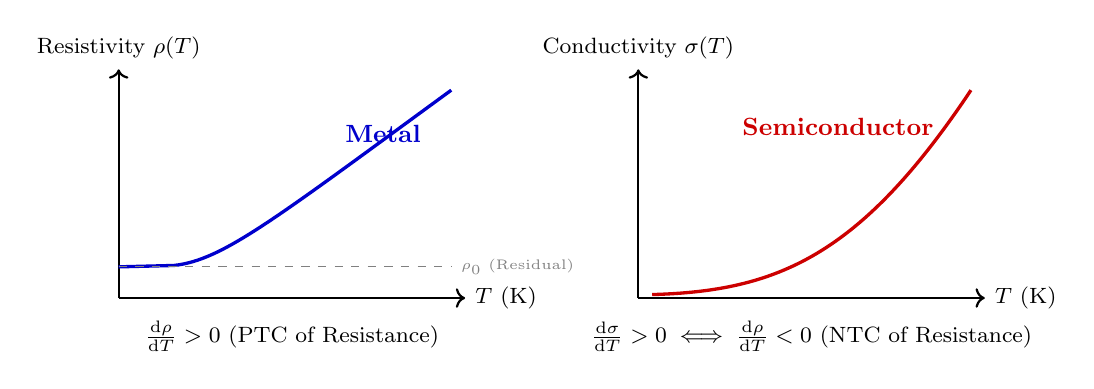
\begin{tikzpicture}[scale=0.88]
  \begin{scope}[shift={(0,0)}]
    \draw[->,thick] (0,0) -- (5.0,0) node[right,font=\footnotesize] {$T$ (K)};
    \draw[->,thick] (0,0) -- (0,3.3) node[above,font=\footnotesize] {Resistivity $\rho(T)$};
    \draw[blue!80!black,very thick] (0,0.45) -- (0.8,0.47) .. controls (1.5,0.55) and (2.2,1.1) .. (4.8,3.0);
    \draw[dashed,gray] (0,0.45) -- (4.8,0.45) node[right,font=\tiny] {$\rho_0$ (Residual)};
    \node[blue!80!black,above left,font=\small] at (4.5,2.1) {\textbf{Metal}};
    \node[font=\footnotesize,align=center] at (2.5,-0.55) {$\dv{\rho}{T} > 0$ (PTC of Resistance)};
  \end{scope}
  \begin{scope}[shift={(7.5,0)}]
    \draw[->,thick] (0,0) -- (5.0,0) node[right,font=\footnotesize] {$T$ (K)};
    \draw[->,thick] (0,0) -- (0,3.3) node[above,font=\footnotesize] {Conductivity $\sigma(T)$};
    \draw[red!80!black,very thick] (0.2,0.05) .. controls (2.0,0.1) and (3.2,0.6) .. (4.8,3.0);
    \node[red!80!black,above left,font=\small] at (4.4,2.2) {\textbf{Semiconductor}};
    \node[font=\footnotesize,align=center] at (2.5,-0.55) {$\dv{\sigma}{T} > 0 \iff \dv{\rho}{T} < 0$ (NTC of Resistance)};
  \end{scope}
\end{tikzpicture}
\caption{Temperature dependence of electrical transport in (left) a metal and (right) an intrinsic semiconductor.}
\label{fig:rho_sigma_temp_master}
\end{figure}

\subsection{Crystal Structure, \texorpdfstring{$sp^3$}{sp3} Hybridization, and Compound Semiconductors}
Elemental Group IV semiconductors ($\text{Si}: [\text{Ne}]\,3s^2 3p^2$; $\text{Ge}: [\text{Ar}]\,3d^{10}4s^2 4p^2$) crystallize in the **diamond cubic lattice** (FCC Bravais lattice with a 2-atom basis at $(0,0,0)$ and $(\frac{1}{4},\frac{1}{4},\frac{1}{4})a$). One $s$-electron promotes to the $p$-subshell ($s^2p^2 \to s^1p_x^1p_y^1p_z^1$) to form four directed tetrahedral $sp^3$ hybrid orbitals separated by $\theta = \arccos(-1/3) = 109^\circ 28'$:
\begin{align}
    \ket{h_1} &= \frac{1}{2}\big(\ket{s}+\ket{p_x}+\ket{p_y}+\ket{p_z}\big), & \ket{h_2} &= \frac{1}{2}\big(\ket{s}+\ket{p_x}-\ket{p_y}-\ket{p_z}\big), \\
    \ket{h_3} &= \frac{1}{2}\big(\ket{s}-\ket{p_x}+\ket{p_y}-\ket{p_z}\big), & \ket{h_4} &= \frac{1}{2}\big(\ket{s}-\ket{p_x}-\ket{p_y}+\ket{p_z}\big).
\end{align}
Compound semiconductors maintain an average of $4$ valence electrons per atom: **III--V compounds** ($\text{GaAs}, \text{InP}, \text{InSb}$, zincblende structure, $\frac{3+5}{2}=4$), **II--VI compounds** ($\text{CdS}, \text{CdTe}, \text{ZnS}$, zincblende/wurtzite, $\frac{2+6}{2}=4$), and **amorphous chalcogenide glasses** (Group VI $\text{S}, \text{Se}, \text{Te}$ networks such as $\text{As}_2\text{Se}_3$).

\begin{figure}[htbp]
\centering
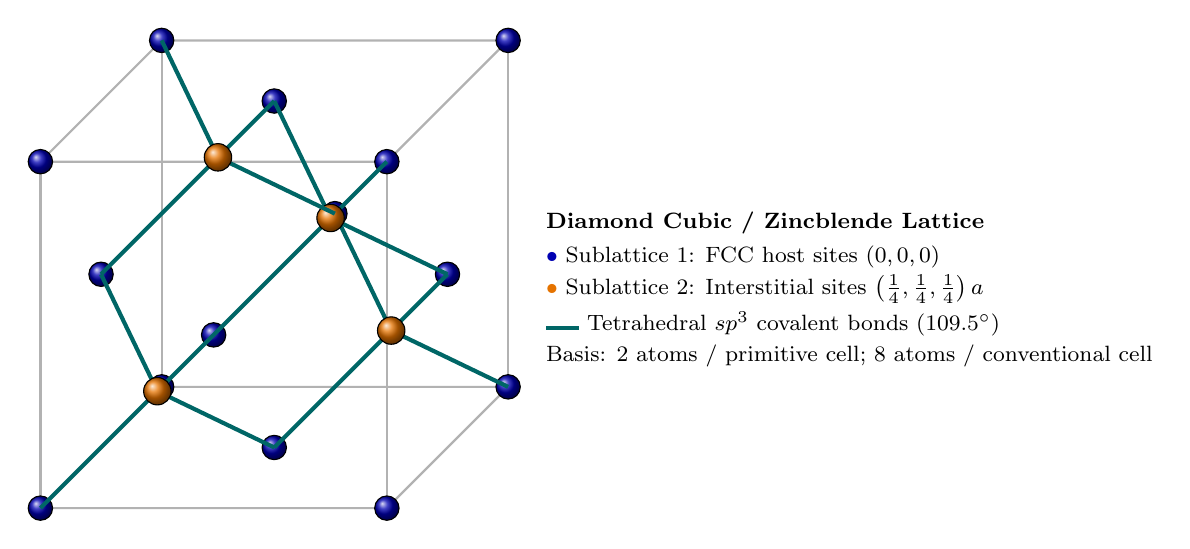
\begin{tikzpicture}[scale=1.1, >=Stealth, x={(1cm,0cm)}, y={(0.35cm,0.35cm)}, z={(0cm,1cm)}]
  % Wireframe of conventional cubic cell
  \draw[thick, gray!60] (0,0,0) -- (4,0,0) -- (4,4,0) -- (0,4,0) -- cycle;
  \draw[thick, gray!60] (0,0,4) -- (4,0,4) -- (4,4,4) -- (0,4,4) -- cycle;
  \draw[thick, gray!60] (0,0,0) -- (0,0,4);
  \draw[thick, gray!60] (4,0,0) -- (4,0,4);
  \draw[thick, gray!60] (4,4,0) -- (4,4,4);
  \draw[thick, gray!60] (0,4,0) -- (0,4,4);

  % FCC Sublattice 1 (Corners and Face Centers) - Blue
  % 8 Corners
  \foreach \x in {0,4} \foreach \y in {0,4} \foreach \z in {0,4} {
    \filldraw[ball color=blue!70!black] (\x,\y,\z) circle (4pt);
  }
  % 6 Face centers
  \filldraw[ball color=blue!70!black] (2,2,0) circle (4pt);
  \filldraw[ball color=blue!70!black] (2,2,4) circle (4pt);
  \filldraw[ball color=blue!70!black] (2,0,2) circle (4pt);
  \filldraw[ball color=blue!70!black] (2,4,2) circle (4pt);
  \filldraw[ball color=blue!70!black] (0,2,2) circle (4pt);
  \filldraw[ball color=blue!70!black] (4,2,2) circle (4pt);

  % FCC Sublattice 2 (Tetrahedral Interstitial Basis Atoms shifted by (1/4, 1/4, 1/4)a) - Gold/Orange
  % Bonds from basis atoms to 4 nearest neighbors
  % Basis atom 1: (1,1,1)
  \draw[line width=1.5pt, teal!80!black] (1,1,1) -- (0,0,0);
  \draw[line width=1.5pt, teal!80!black] (1,1,1) -- (2,2,0);
  \draw[line width=1.5pt, teal!80!black] (1,1,1) -- (2,0,2);
  \draw[line width=1.5pt, teal!80!black] (1,1,1) -- (0,2,2);
  \filldraw[ball color=orange!90!black] (1,1,1) circle (4.5pt);

  % Basis atom 2: (3,3,1)
  \draw[line width=1.5pt, teal!80!black] (3,3,1) -- (4,4,0);
  \draw[line width=1.5pt, teal!80!black] (3,3,1) -- (2,2,0);
  \draw[line width=1.5pt, teal!80!black] (3,3,1) -- (4,2,2);
  \draw[line width=1.5pt, teal!80!black] (3,3,1) -- (2,4,2);
  \filldraw[ball color=orange!90!black] (3,3,1) circle (4.5pt);

  % Basis atom 3: (3,1,3)
  \draw[line width=1.5pt, teal!80!black] (3,1,3) -- (4,0,4);
  \draw[line width=1.5pt, teal!80!black] (3,1,3) -- (2,2,4);
  \draw[line width=1.5pt, teal!80!black] (3,1,3) -- (4,2,2);
  \draw[line width=1.5pt, teal!80!black] (3,1,3) -- (2,0,2);
  \filldraw[ball color=orange!90!black] (3,1,3) circle (4.5pt);

  % Basis atom 4: (1,3,3)
  \draw[line width=1.5pt, teal!80!black] (1,3,3) -- (0,4,4);
  \draw[line width=1.5pt, teal!80!black] (1,3,3) -- (2,2,4);
  \draw[line width=1.5pt, teal!80!black] (1,3,3) -- (0,2,2);
  \draw[line width=1.5pt, teal!80!black] (1,3,3) -- (2,4,2);
  \filldraw[ball color=orange!90!black] (1,3,3) circle (4.5pt);

  % Legend / annotations
  \node[anchor=west,font=\footnotesize,align=left] at (5.2,1.5,2) {
    \textbf{Diamond Cubic / Zincblende Lattice}\\[3pt]
    {\color{blue!70!black}$\bullet$} Sublattice 1: FCC host sites ($0,0,0$)\\[2pt]
    {\color{orange!90!black}$\bullet$} Sublattice 2: Interstitial sites $\left(\frac{1}{4},\frac{1}{4},\frac{1}{4}\right)a$\\[2pt]
    {\color{teal!80!black}\rule{12pt}{1.5pt}} Tetrahedral $sp^3$ covalent bonds ($109.5^\circ$)\\[2pt]
    Basis: 2 atoms / primitive cell; 8 atoms / conventional cell
  };
\end{tikzpicture}
\caption{Conventional unit cell of the Diamond Cubic lattice (Silicon, Germanium) and Zincblende structure ($\text{GaAs}$, $\text{InP}$). Two interpenetrating FCC sublattices are displaced along the body diagonal by $(\frac{a}{4}, \frac{a}{4}, \frac{a}{4})$, creating four-fold tetrahedral coordination.}
\label{fig:diamond_cubic_wireframe_master}
\end{figure}

\subsection{Intrinsic Semiconductors: Complete Derivation of Carrier Densities \texorpdfstring{$n, p, n_i$}{n, p, n_i} and \texorpdfstring{$E_F$}{E_F}}
\subsubsection{Step 1: 3D Density of States Near Parabolic Band Edges}
Near the conduction band minimum $E_c$ and valence band maximum $E_v$, the dispersions are parabolic:
\begin{equation}
    E_e(\kk) = E_c + \frac{\hbarsq k^2}{2m_e^*}, \qquad E_h(\kk) = E_v - \frac{\hbarsq k^2}{2m_h^*}.
\end{equation}
In 3D $\kk$-space, the number of orbital states per unit volume in a spherical shell $(k, k+\dd k)$ including spin ($g_s = 2$) is:
\begin{equation}
    g(k)\,\dd k = 2 \times \frac{4\pi k^2\,\dd k}{(2\pi)^3} = \frac{k^2\,\dd k}{\pi^2}.
\end{equation}
Substituting $k = \left[\frac{2m_e^*(E-E_c)}{\hbarsq}\right]^{1/2}$ and $\dd k = \frac{1}{2}\left(\frac{2m_e^*}{\hbarsq}\right)^{1/2}(E-E_c)^{-1/2}\dd E$ gives the 3D densities of states per unit volume:
\begin{align}
    \boxed{g_c(E) = \frac{1}{2\pi^2}\left(\frac{2m_e^*}{\hbarsq}\right)^{3/2}(E - E_c)^{1/2} = 4\pi\left(\frac{2m_e^*}{h^2}\right)^{3/2}(E - E_c)^{1/2} \qquad (E \ge E_c),} \\
    \boxed{g_v(E) = \frac{1}{2\pi^2}\left(\frac{2m_h^*}{\hbarsq}\right)^{3/2}(E_v - E)^{1/2} = 4\pi\left(\frac{2m_h^*}{h^2}\right)^{3/2}(E_v - E)^{1/2} \qquad (E \le E_v).}
\end{align}

\subsubsection{Step 2: Non-Degenerate Fermi--Dirac Integrals via Euler's Gamma Function}
In a non-degenerate semiconductor where $E_c - E_F \gg k_B T$ and $E_F - E_v \gg k_B T$, the Fermi--Dirac probabilities reduce to Boltzmann tails:
\begin{equation}
    f_e(E) = \frac{1}{e^{(E-E_F)/k_BT} + 1} \approx e^{-(E-E_F)/k_BT}, \qquad f_h(E) = 1 - f_e(E) = \frac{1}{e^{(E_F-E)/k_BT} + 1} \approx e^{-(E_F-E)/k_BT}.
\end{equation}
Integrating over the conduction band using $x \equiv \frac{E - E_c}{k_B T}$ ($\dd E = k_B T\,\dd x$) and $\int_0^\infty x^{1/2}e^{-x}\,\dd x = \Gamma(3/2) = \frac{\sqrt{\pi}}{2}$:
\begin{align}
    n &= \int_{E_c}^\infty g_c(E)f_e(E)\,\dd E = \frac{1}{2\pi^2}\left(\frac{2m_e^*}{\hbarsq}\right)^{3/2} e^{-(E_c-E_F)/k_BT} (k_B T)^{3/2}\underbrace{\int_0^\infty x^{1/2}e^{-x}\,\dd x}_{=\sqrt{\pi}/2} \notag\\
    &= \underbrace{2\left(\frac{m_e^* k_B T}{2\pi\hbarsq}\right)^{3/2}}_{\equiv\, N_c} \exp\left(-\frac{E_c - E_F}{k_B T}\right) = N_c \exp\left(-\frac{E_c - E_F}{k_B T}\right).
    \label{eq:n_master}
\end{align}
Similarly, integrating over the valence band with $y \equiv \frac{E_v - E}{k_B T}$ gives the hole concentration:
\begin{equation}
    p = \int_{-\infty}^{E_v} g_v(E)f_h(E)\,\dd E = \underbrace{2\left(\frac{m_h^* k_B T}{2\pi\hbarsq}\right)^{3/2}}_{\equiv\, N_v} \exp\left(-\frac{E_F - E_v}{k_B T}\right) = N_v \exp\left(-\frac{E_F - E_v}{k_B T}\right).
    \label{eq:p_master}
\end{equation}

\subsubsection{Step 3: Law of Mass Action, Intrinsic Carrier Density \texorpdfstring{$n_i$}{n_i}, and Intrinsic Fermi Level}
Multiplying Eqs.~\eqref{eq:n_master} and \eqref{eq:p_master} cancels $E_F$ identically ($E_g \equiv E_c - E_v$), establishing the **Law of Mass Action**:
\begin{equation}
    \boxed{n \cdot p = N_c N_v \exp\left(-\frac{E_c - E_v}{k_B T}\right) = N_c N_v \exp\left(-\frac{E_g}{k_B T}\right) = n_i^2(T),}
    \label{eq:mass_action_master}
\end{equation}
\begin{equation}
    \boxed{n_i(T) = \sqrt{N_c N_v}\exp\left(-\frac{E_g}{2k_B T}\right) = 2\left(\frac{k_B T}{2\pi\hbarsq}\right)^{3/2}(m_e^* m_h^*)^{3/4}\exp\left(-\frac{E_g}{2k_B T}\right).}
    \label{eq:ni_master}
\end{equation}
Setting $n = p$ in an intrinsic semiconductor gives $N_c e^{-(E_c-E_i)/k_BT} = N_v e^{-(E_i-E_v)/k_BT}$. Taking the natural logarithm yields the **intrinsic Fermi level** $E_i \equiv E_F^{\mathrm{int}}$:
\begin{equation}
    \boxed{E_i = \frac{E_c + E_v}{2} + \frac{1}{2}k_B T \ln\left(\frac{N_v}{N_c}\right) = \frac{E_c + E_v}{2} + \frac{3}{4}k_B T \ln\left(\frac{m_h^*}{m_e^*}\right).}
    \label{eq:Ei_master}
\end{equation}
The intrinsic electrical conductivity is $\sigma_i = n_i e(\mu_e + \mu_h) = \sigma_0 e^{-E_g/(2k_B T)}$, so a plot of $\ln\sigma_i$ vs.\ $1/T$ has slope $-\frac{E_g}{2k_B}$.

\subsection{Extrinsic Semiconductors: Hydrogenic Impurity Model and Carrier Statistics}
\subsubsection{Hydrogenic Model of Shallow Donors and Acceptors}
When a pentavalent Group V donor ($\text{P}, \text{As}, \text{Sb}$) substitutes for a $\text{Si}$ atom, four valence electrons form covalent bonds and the fifth electron orbits the fixed $\text{P}^+$ ion core inside the dielectric medium ($\epsilon = \epsilon_r\epsilon_0$) with effective mass $m_e^*$. Replacing $\epsilon_0 \to \epsilon_r\epsilon_0$ and $m_0 \to m_e^*$ in the Bohr hydrogen atom formulas yields the **donor ionization energy** $\Delta E_d = E_c - E_d$ and **effective Bohr radius** $r_d^*$:
\begin{equation}
    \boxed{\Delta E_d = \frac{m_e^* e^4}{2(4\pi\epsilon_r\epsilon_0\hb)^2} = \left(\frac{m_e^*}{m_0}\right)\frac{13.6\ \mathrm{eV}}{\epsilon_r^2}, \qquad r_d^* = a_0\,\epsilon_r\left(\frac{m_0}{m_e^*}\right) \quad (a_0 = 0.529\ \text{\AA}).}
    \label{eq:hydrogenic_master}
\end{equation}
For $\text{Si}$ ($\epsilon_r = 11.7$, $m_e^* = 0.26\,m_0$), $\Delta E_d \approx 25.8\ \mathrm{meV} \sim k_B T(300\ \mathrm{K})$ and $r_d^* \approx 23.9\ \text{\AA}$ (spanning $\sim 9$ lattice constants). At heavy doping ($N_d \gtrsim 10^{18}\ \mathrm{cm^{-3}}$), neighboring donor orbitals overlap ($N_d^{-1/3} \lesssim 2r_d^*$) to form an **impurity band** (**Mott transition**).

\subsubsection{Rigorous Derivation of the Extrinsic Carrier Quadratic Equation and Three Temperature Regimes}
Macroscopic charge neutrality requires:
\begin{equation}
    \boxed{n + N_a^- = p + N_d^+.}
    \label{eq:neutrality_master}
\end{equation}
A neutral donor level at $E_d$ accommodates one electron with spin up or spin down ($g_d = 2$), but forbids double occupancy due to strong Coulomb repulsion. Its grand partition function is $\mathcal{Z}_d = 1 + 2e^{(E_F - E_d)/k_BT}$, so the neutral and ionized donor concentrations ($N_d = N_d^0 + N_d^+$) are:
\begin{equation}
    N_d^0 = \frac{N_d}{1 + \frac{1}{2}e^{(E_d - E_F)/k_BT}}, \qquad N_d^+ = \frac{N_d}{1 + 2e^{(E_F - E_d)/k_BT}} \implies \frac{N_d^0}{N_d^+} = 2\exp\left(\frac{E_F - E_d}{k_B T}\right).
\end{equation}
Substituting $e^{E_F/k_BT} = \frac{n}{N_c}e^{E_c/k_BT}$ from Eq.~\eqref{eq:n_master} into $\frac{N_d^0}{N_d^+}$ ($\Delta E_d \equiv E_c - E_d$):
\begin{equation}
    \frac{N_d^0}{N_d^+} = \frac{2n}{N_c}\exp\left(\frac{\Delta E_d}{k_B T}\right) = \frac{n}{K_d(T)}, \qquad \text{where } \boxed{K_d(T) \equiv \frac{1}{2}N_c\exp\left(-\frac{\Delta E_d}{k_B T}\right).}
\end{equation}
For an uncompensated $n$-type semiconductor ($N_a = 0$) below the intrinsic regime ($p \ll n$), charge neutrality gives $n = N_d^+$ and $N_d^0 = N_d - n$. Substituting these into $\frac{N_d^0}{N_d^+} = \frac{n}{K_d}$ gives $\frac{N_d - n}{n} = \frac{n}{K_d}$, which rearranges into the **fundamental quadratic equation for extrinsic electron concentration**:
\begin{equation}
    \boxed{n^2 + K_d(T)\,n - K_d(T)\,N_d = 0 \implies n(T) = \frac{K_d}{2}\left[\sqrt{1 + \frac{4N_d}{K_d}} - 1\right].}
    \label{eq:quadratic_n_master}
\end{equation}

\paragraph{The Three Characteristic Temperature Regimes (Figure~\ref{fig:arrhenius_master}):}
\begin{enumerate}
    \item \textbf{Regime I: Low-Temperature Freeze-Out Range ($k_B T \ll \Delta E_d$, so $\frac{4N_d}{K_d} \gg 1$):}
    \begin{equation}
        n(T) \approx \frac{K_d}{2}\sqrt{\frac{4N_d}{K_d}} = \sqrt{K_d N_d} = \boxed{\sqrt{\frac{N_c N_d}{2}}\exp\left(-\frac{\Delta E_d}{2k_B T}\right), \qquad E_F(T) = E_c - \frac{\Delta E_d}{2} + \frac{1}{2}k_B T\ln\left(\frac{N_d}{2N_c}\right).}
    \end{equation}
    Arrhenius slope of $\ln n$ vs.\ $1/T$ is $-\frac{\Delta E_d}{2k_B}$, and $E_F \to \frac{E_c + E_d}{2}$ as $T \to 0\ \mathrm{K}$.
    \item \textbf{Regime II: Intermediate-Temperature Saturation / Exhaustion Range ($\Delta E_d \ll k_B T \ll E_g$, so $\frac{4N_d}{K_d} \ll 1$):}
    Expanding $\sqrt{1 + \frac{4N_d}{K_d}} \approx 1 + \frac{2N_d}{K_d}$ in Eq.~\eqref{eq:quadratic_n_master} (or including compensation $N_a < N_d$ and $np = n_i^2$):
    \begin{equation}
        \boxed{n(T) \approx N_d \quad (\text{or } n = \frac{N_d - N_a}{2} + \sqrt{\left(\frac{N_d - N_a}{2}\right)^2 + n_i^2}), \qquad p = \frac{n_i^2}{n}, \qquad E_F = E_c - k_B T\ln\left(\frac{N_c}{n}\right).}
    \end{equation}
    \item \textbf{Regime III: High-Temperature Intrinsic Range ($k_B T$ large enough that $n_i(T) \gg N_d$):}
    Thermal excitation across $E_g$ overwhelms the dopant density: $n \approx p \approx n_i(T) = \sqrt{N_c N_v}e^{-E_g/(2k_B T)}$ with steep Arrhenius slope $-\frac{E_g}{2k_B}$ and $E_F \to E_i$.
\end{enumerate}

\begin{figure}[htbp]
\centering
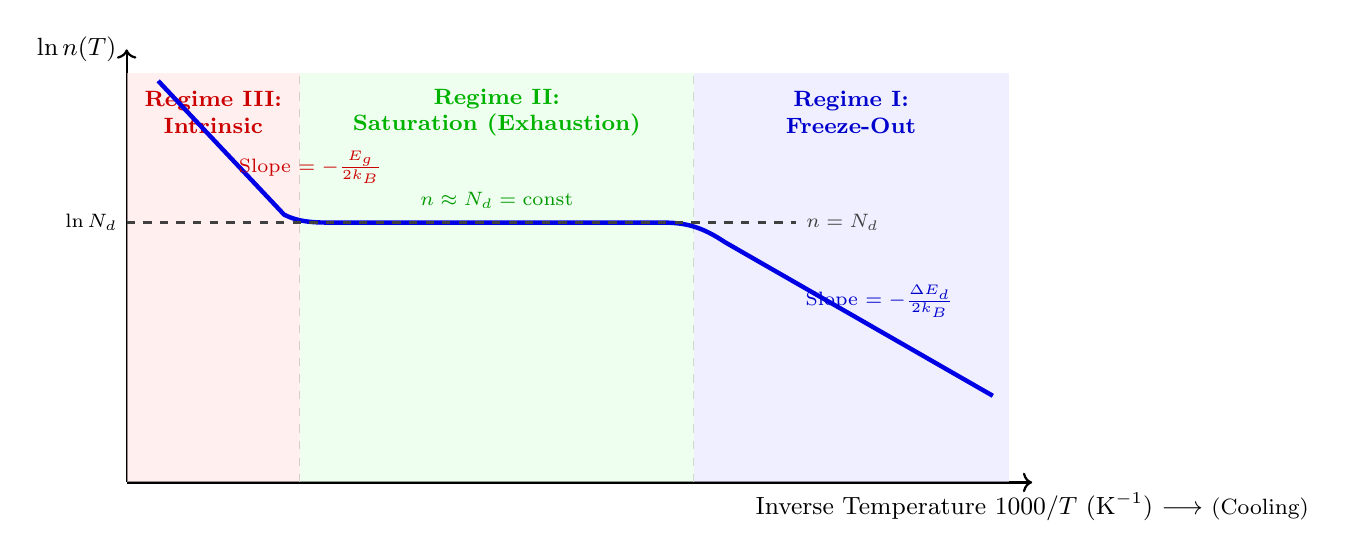
\begin{tikzpicture}[scale=1.0]
  \draw[->,thick] (0,0) -- (11.5,0) node[below,font=\small] {Inverse Temperature $1000/T$ (K$^{-1}$) $\longrightarrow$ \footnotesize(Cooling)};
  \draw[->,thick] (0,0) -- (0,5.5) node[left,font=\small] {$\ln n(T)$};
  \draw[dashed,gray!70] (2.2,0) -- (2.2,5.2);
  \draw[dashed,gray!70] (7.2,0) -- (7.2,5.2);
  \fill[red!10,opacity=0.6] (0,0) rectangle (2.2,5.2);
  \fill[green!10,opacity=0.6] (2.2,0) rectangle (7.2,5.2);
  \fill[blue!10,opacity=0.6] (7.2,0) rectangle (11.2,5.2);
  \node[font=\footnotesize\bfseries,align=center,red!80!black] at (1.1,4.7) {Regime III:\\Intrinsic};
  \node[font=\footnotesize\bfseries,align=center,green!70!black] at (4.7,4.7) {Regime II:\\Saturation (Exhaustion)};
  \node[font=\footnotesize\bfseries,align=center,blue!80!black] at (9.2,4.7) {Regime I:\\Freeze-Out};
  \draw[ultra thick,blue!90!black] 
    (0.4,5.1) -- (2.0,3.4) 
    .. controls (2.2,3.3) and (2.4,3.3) .. (2.6,3.3)
    -- (6.8,3.3)
    .. controls (7.1,3.3) and (7.3,3.25) .. (7.6,3.05)
    -- (11.0,1.1);
  \draw[dashed,darkgray,thick] (0,3.3) -- (8.5,3.3) node[right,font=\scriptsize] {$n = N_d$};
  \node[left,font=\scriptsize] at (0,3.3) {$\ln N_d$};
  \node[red!80!black,right,font=\scriptsize] at (1.3,4.0) {Slope $= -\frac{E_g}{2 k_B}$};
  \node[green!60!black,above,font=\scriptsize] at (4.7,3.35) {$n \approx N_d = \text{const}$};
  \node[blue!80!black,right,font=\scriptsize] at (8.5,2.3) {Slope $= -\frac{\Delta E_d}{2 k_B}$};
\end{tikzpicture}
\caption{Arrhenius plot of $\ln n$ versus $1000/T$ for an $n$-type semiconductor across the Freeze-Out, Saturation (Exhaustion), and Intrinsic regimes.}
\label{fig:arrhenius_master}
\end{figure}

\subsection{Direct vs.\ Indirect Band Gap Optical Transitions}
Because a photon of optical wavelength $\lambda \sim 1\ \mu\mathrm{m}$ has wavevector $q_{\mathrm{photon}} = \frac{2\pi}{\lambda} \sim 6 \times 10^6\ \mathrm{m^{-1}} \ll \frac{\pi}{a} \sim 6 \times 10^9\ \mathrm{m^{-1}}$, photon absorption is vertical in $\kk$-space ($\Delta\kk = \vb{q}_{\mathrm{photon}} \approx \vb{0}$, Figure~\ref{fig:direct_indirect_master}):
\begin{itemize}
    \item \textbf{Direct Gap ($\text{GaAs}, \text{InP}$):} $E_c$ minimum and $E_v$ maximum occur at the same $\kk = \vb{0}$ ($\Gamma$-point). First-order vertical photon transition: $\hb\omega_{\mathrm{th}} = E_g$, $\alpha(\omega) \propto (\hb\omega - E_g)^{1/2}$. Ideal for LEDs and lasers.
    \item \textbf{Indirect Gap ($\text{Si}, \text{Ge}$):} $E_c$ minimum sits at $\kk_{\min} \neq \vb{0}$, requiring simultaneous absorption/emission of a phonon of wavevector $\vb{q}_{\mathrm{ph}} = \kk_{\min}$ and energy $\hb\Omega_{\mathrm{ph}}$: $\hb\omega = E_g \pm \hb\Omega_{\mathrm{ph}}$, $\alpha(\omega) \propto (\hb\omega - E_g \mp \hb\Omega_{\mathrm{ph}})^2$.
\end{itemize}

\begin{figure}[htbp]
\centering
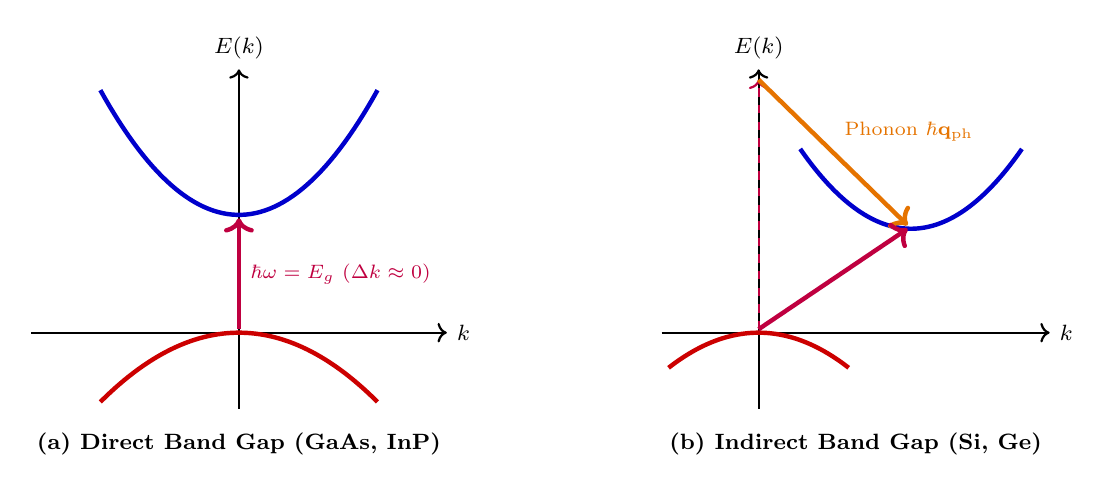
\begin{tikzpicture}[scale=0.88]
  \begin{scope}[shift={(0,0)}]
    \draw[->,thick] (-3.0,0) -- (3.0,0) node[right,font=\footnotesize] {$k$};
    \draw[->,thick] (0,-1.1) -- (0,3.8) node[above,font=\footnotesize] {$E(k)$};
    \draw[blue!80!black,ultra thick] plot[domain=-2.0:2.0,samples=60] (\x,{1.7 + 0.45*\x*\x});
    \draw[red!80!black,ultra thick] plot[domain=-2.0:2.0,samples=60] (\x,{0.0 - 0.25*\x*\x});
    \draw[->,purple,ultra thick] (0,0.05) -- (0,1.65) node[midway,right,font=\scriptsize] {$\hb\omega = E_g$ ($\Delta k \approx 0$)};
    \node[below,font=\footnotesize\bfseries] at (0,-1.3) {(a) Direct Band Gap ($\text{GaAs}$, $\text{InP}$)};
  \end{scope}
  \begin{scope}[shift={(7.5,0)}]
    \draw[->,thick] (-1.4,0) -- (4.2,0) node[right,font=\footnotesize] {$k$};
    \draw[->,thick] (0,-1.1) -- (0,3.8) node[above,font=\footnotesize] {$E(k)$};
    \draw[red!80!black,ultra thick] plot[domain=-1.3:1.3,samples=60] (\x,{0.0 - 0.3*\x*\x});
    \draw[blue!80!black,ultra thick] plot[domain=0.6:3.8,samples=60] (\x,{1.5 + 0.45*(\x - 2.2)*(\x - 2.2)});
    \draw[->,purple,thick,dashed] (0,0.05) -- (0,3.65);
    \draw[->,orange!90!black,ultra thick] (0,3.65) -- (2.15,1.55) node[midway,above right,font=\scriptsize] {Phonon $\hb\vb{q}_{\mathrm{ph}}$};
    \draw[->,purple,ultra thick] (0,0.05) -- (2.15,1.5);
    \node[below,font=\footnotesize\bfseries] at (1.4,-1.3) {(b) Indirect Band Gap ($\text{Si}$, $\text{Ge}$)};
  \end{scope}
\end{tikzpicture}
\caption{Optical absorption in (a) a direct-gap semiconductor ($\Delta\kk \approx \vb{0}$) and (b) an indirect-gap semiconductor requiring phonon momentum conservation.}
\label{fig:direct_indirect_master}
\end{figure}

\begin{figure}[htbp]
\centering
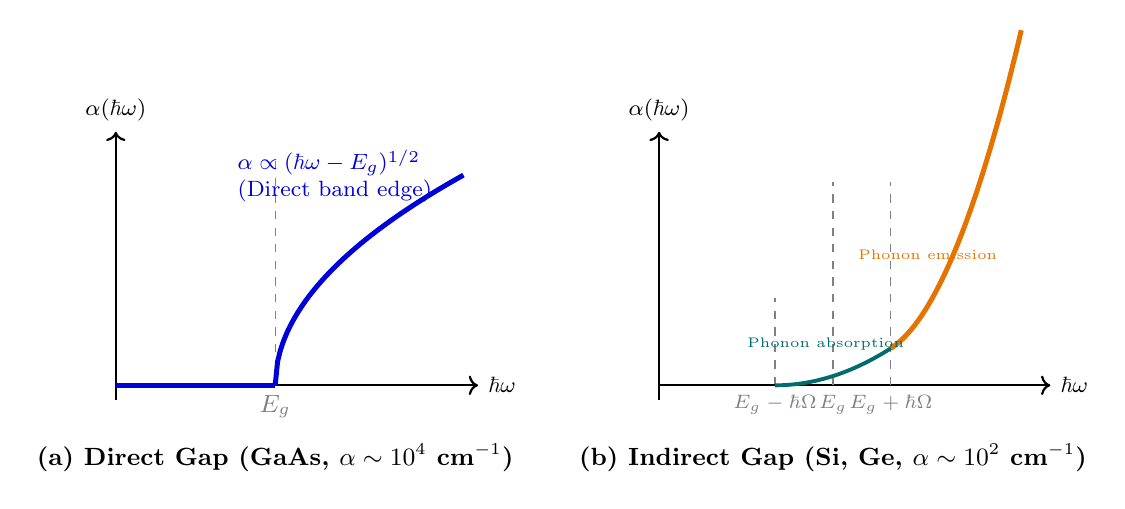
\begin{tikzpicture}[scale=0.92]
  % (a) Direct Gap
  \begin{scope}[xshift=0cm]
    \draw[->,thick] (0,0) -- (5.0,0) node[right,font=\footnotesize] {$\hbar\omega$};
    \draw[->,thick] (0,-0.2) -- (0,3.5) node[above,font=\footnotesize] {$\alpha(\hbar\omega)$};
    \draw[dashed,gray] (2.2,0) node[below,font=\small] {$E_g$} -- (2.2,3.2);

    % Sharp onset: sqrt(hbar omega - Eg)
    \draw[line width=1.8pt,blue!85!black,domain=2.2:4.8,samples=80]
      plot (\x, {1.8*sqrt(\x - 2.2)});
    \draw[line width=1.8pt,blue!85!black] (0,0) -- (2.2,0);

    \node[above left,font=\footnotesize,blue!85!black,align=left] at (4.5,2.4) {$\alpha \propto (\hbar\omega - E_g)^{1/2}$\\(Direct band edge)};
    \node[font=\bfseries\small] at (2.2,-1.0) {(a) Direct Gap ($\text{GaAs}$, $\alpha \sim 10^4\text{ cm}^{-1}$)};
  \end{scope}

  % (b) Indirect Gap
  \begin{scope}[xshift=7.5cm]
    \draw[->,thick] (0,0) -- (5.4,0) node[right,font=\footnotesize] {$\hbar\omega$};
    \draw[->,thick] (0,-0.2) -- (0,3.5) node[above,font=\footnotesize] {$\alpha(\hbar\omega)$};

    \draw[dashed,gray] (1.6,0) node[below,font=\scriptsize] {$E_g - \hbar\Omega$} -- (1.6,1.2);
    \draw[dashed,gray] (2.4,0) node[below,font=\scriptsize] {$E_g$} -- (2.4,2.8);
    \draw[dashed,gray] (3.2,0) node[below,font=\scriptsize] {$E_g + \hbar\Omega$} -- (3.2,2.8);

    % First knee: phonon absorption (Eg - hbar Omega)
    \draw[line width=1.4pt,teal!85!black,domain=1.6:3.2,samples=60]
      plot (\x, {0.2*(\x - 1.6)*(\x - 1.6)});

    % Second knee: phonon emission (Eg + hbar Omega)
    \draw[line width=1.8pt,orange!90!black,domain=3.2:5.0,samples=80]
      plot (\x, {0.2*(\x - 1.6)*(\x - 1.6) + 0.8*(\x - 3.2)*(\x - 3.2)});

    \draw[thick,black] (0,0) -- (1.6,0);

    \node[above,font=\tiny,teal!85!black] at (2.3,0.35) {Phonon absorption};
    \node[above left,font=\tiny,orange!90!black] at (4.8,1.6) {Phonon emission};
    \node[font=\bfseries\small] at (2.4,-1.0) {(b) Indirect Gap ($\text{Si}$, $\text{Ge}$, $\alpha \sim 10^2\text{ cm}^{-1}$)};
  \end{scope}
\end{tikzpicture}
\caption{Comparison of optical absorption coefficient spectra $\alpha(\hbar\omega)$. (a) Direct-gap semiconductor showing an abrupt onset $\alpha \propto (\hbar\omega-E_g)^{1/2}$ at $\hbar\omega = E_g$. (b) Indirect-gap semiconductor showing two characteristic threshold knees corresponding to phonon absorption at $\hbar\omega = E_g - \hbar\Omega$ and phonon emission at $\hbar\omega = E_g + \hbar\Omega$.}
\label{fig:optical_absorption_spectra_master}
\end{figure}

\subsection{The Classical Hall Effect in Semiconductors}
Consider a rectangular semiconductor bar of width $w$ (along $y$) and thickness $t$ (along $z$) carrying current $I_x$ ($j_x = \frac{I_x}{wt}$) along $+x$ in a perpendicular magnetic field $\vb{B} = B_z\hat{\vb{z}}$ (Figure~\ref{fig:hall_geometry_master}).

\begin{figure}[htbp]
\centering
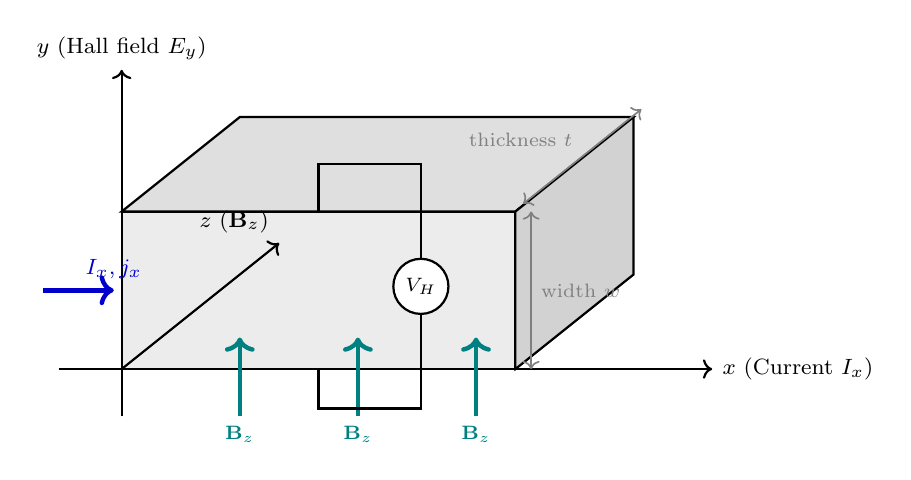
\begin{tikzpicture}[scale=1.0]
  \draw[thick,fill=gray!15] (0,0) -- (5,0) -- (5,2) -- (0,2) -- cycle;
  \draw[thick,fill=gray!25] (0,2) -- (5,2) -- (6.5,3.2) -- (1.5,3.2) -- cycle;
  \draw[thick,fill=gray!35] (5,0) -- (6.5,1.2) -- (6.5,3.2) -- (5,2) -- cycle;
  \draw[->,thick,black] (-0.8,0) -- (7.5,0) node[right,font=\footnotesize] {$x$ (Current $I_x$)};
  \draw[->,thick,black] (0,-0.6) -- (0,3.8) node[above,font=\footnotesize] {$y$ (Hall field $E_y$)};
  \draw[->,thick,black] (0,0) -- (2.0,1.6) node[above left,font=\footnotesize] {$z$ ($\vb{B}_z$)};
  \draw[->,ultra thick,blue!80!black] (-1.0,1.0) -- (-0.1,1.0) node[above,font=\footnotesize] {$I_x, j_x$};
  \foreach \x in {1.5, 3.0, 4.5} {
    \draw[->,ultra thick,teal] (\x, -0.6) -- (\x, 0.4);
    \node[teal,below,font=\scriptsize] at (\x,-0.6) {$\vb{B}_z$};
  }
  \draw[thick] (2.5,2.0) -- (2.5,2.6) -- (3.8,2.6) -- (3.8,1.4);
  \draw[thick] (2.5,0.0) -- (2.5,-0.5) -- (3.8,-0.5) -- (3.8,0.7);
  \draw[thick,fill=white] (3.8,1.05) circle (0.35) node[font=\scriptsize] {$V_H$};
  \draw[<->,gray,semithick] (5.2,0) -- (5.2,2) node[midway,right,font=\scriptsize] {width $w$};
  \draw[<->,gray,semithick] (5.1,2.1) -- (6.6,3.3) node[midway,above left,font=\scriptsize] {thickness $t$};
\end{tikzpicture}
\caption{Orthogonal Hall effect geometry on a rectangular semiconductor bar of width $w$ and thickness $t$.}
\label{fig:hall_geometry_master}
\end{figure}

\subsubsection{Lorentz Force Equilibrium, Hall Coefficient \texorpdfstring{$R_H$}{R_H}, Hall Voltage \texorpdfstring{$V_H$}{V_H}, and Hall Mobility \texorpdfstring{$\mu_H$}{mu_H}}
A carrier of charge $q$ drifting with velocity $\vb{v} = (v_x, v_y, 0)$ experiences Lorentz force $\vb{F} = q(\vb{E} + \vb{v}\times\vb{B})$, whose $y$-component is $F_y = q(E_y - v_x B_z)$. Both electrons ($q = -e, v_x < 0$) and holes ($q = +e, v_x > 0$) experience a magnetic force $F_{\mathrm{mag},y} = -qv_x B_z = -j_x B_z / n < 0$ deflecting them toward the $-y$ face! In steady state ($v_y = 0, F_y = 0$), the transverse Hall electric field $E_y$ balances the magnetic deflection:
\begin{equation}
    E_y = v_x B_z = \left(\frac{j_x}{nq}\right)B_z \implies \boxed{R_H \equiv \frac{E_y}{j_x B_z} = \frac{1}{nq} = \begin{cases} -\dfrac{1}{ne} < 0 & (\text{electrons, } n\text{-type}), \\[8pt] +\dfrac{1}{pe} > 0 & (\text{holes, } p\text{-type}). \end{cases}}
\end{equation}
The measurable **Hall voltage** $V_H = E_y w$ across width $w$ and the **Hall mobility** $\mu_H$ (using $\sigma = n\abs{q}\mu$) are:
\begin{equation}
    \boxed{V_H = E_y w = R_H\left(\frac{I_x}{wt}\right)B_z w = \frac{R_H I_x B_z}{t}, \qquad \mu_H \equiv \abs{R_H}\sigma = \left(\frac{1}{n\abs{q}}\right)(n\abs{q}\mu) = \mu.}
\end{equation}

\subsubsection{Two-Carrier Hall Coefficient (Ambipolar Transport)}
When both electrons ($n, \mu_e$) and holes ($p, \mu_h$) conduct simultaneously, their transverse currents cancel ($j_y = j_{e,y} + j_{h,y} = 0$) in the small-field limit ($\mu B \ll 1$), giving the **two-carrier Hall coefficient**:
\begin{equation}
    \boxed{R_H = \frac{p\mu_h^2 - n\mu_e^2}{e(p\mu_h + n\mu_e)^2}.}
    \label{eq:two_carrier_hall_master}
\end{equation}
In an intrinsic semiconductor ($n = p = n_i$), $R_H = -\frac{\mu_e - \mu_h}{n_i e(\mu_e + \mu_h)} < 0$ because $\mu_e > \mu_h$.

\begin{examplebox}{Hall Effect, Carrier Concentration, Mobility, and Compensation in Silicon}{ex:hall_semicon_solved}
\textbf{Problem.} A rectangular bar of doped Silicon at $300\ \mathrm{K}$ ($n_i = 1.5\times 10^{10}\ \mathrm{cm^{-3}}$) has width $w = 4.0\ \mathrm{mm}$, thickness $t = 1.0\ \mathrm{mm}$, and length $L = 1.0\ \mathrm{cm}$. When a current $I_x = 2.0\ \mathrm{mA}$ flows along $x$ in a magnetic field $B_z = 0.50\ \mathrm{T}$, a Hall voltage $V_H = -1.25\ \mathrm{mV}$ is measured across $w$, and the longitudinal voltage drop along $L$ is $V_x = 80\ \mathrm{mV}$. Find: (a) the majority carrier type and concentration, (b) the minority carrier concentration, and (c) the electrical conductivity $\sigma$ and Hall mobility $\mu_H$.
\vspace{0.2cm}\hrule\vspace{0.2cm}
\textbf{Solution.}
\textbf{(a)} Since $V_H < 0$ ($R_H < 0$), the bar is **$n$-type** (electrons are majority carriers):
\[
    R_H = \frac{V_H t}{I_x B_z} = \frac{(-1.25\times 10^{-3}\ \mathrm{V})(1.0\times 10^{-3}\ \mathrm{m})}{(2.0\times 10^{-3}\ \mathrm{A})(0.50\ \mathrm{T})} = \mathbf{-1.25\times 10^{-3}\ \mathrm{m^3/C}},
\]
\[
    n = \frac{1}{e\abs{R_H}} = \frac{1}{(1.602\times 10^{-19}\ \mathrm{C})(1.25\times 10^{-3}\ \mathrm{m^3/C})} = \mathbf{5.00\times 10^{21}\ \mathrm{m^{-3}} = 5.00\times 10^{15}\ \mathrm{cm^{-3}}}.
\]
\textbf{(b)} By the Law of Mass Action, the minority hole concentration is:
\[
    p = \frac{n_i^2}{n} = \frac{(1.5\times 10^{10}\ \mathrm{cm^{-3}})^2}{5.00\times 10^{15}\ \mathrm{cm^{-3}}} = \mathbf{4.50\times 10^{4}\ \mathrm{cm^{-3}}}.
\]
\textbf{(c)} The longitudinal resistance is $R = \frac{V_x}{I_x} = \frac{80\ \mathrm{mV}}{2.0\ \mathrm{mA}} = 40\ \Omega$, so the conductivity and Hall mobility are:
\[
    \sigma = \frac{L}{R w t} = \frac{1.0\times 10^{-2}\ \mathrm{m}}{(40\ \Omega)(4.0\times 10^{-3}\ \mathrm{m})(1.0\times 10^{-3}\ \mathrm{m})} = \mathbf{62.5\ \Omega^{-1}\mathrm{m^{-1}}},
\]
\[
    \mu_H = \abs{R_H}\sigma = (1.25\times 10^{-3}\ \mathrm{m^3/C})(62.5\ \Omega^{-1}\mathrm{m^{-1}}) = \mathbf{0.0781\ \mathrm{m^2/(V\cdot s)} = 781\ \mathrm{cm^2/(V\cdot s)}}.
\]
\end{examplebox}

\subsection{Semiconductor Transport: Drift, Diffusion, and the Einstein Relation}
\label{subsec:semi_transport}

\subsubsection{Drift Velocity, Carrier Mobility, and Electrical Conductivity}
Under an applied electric field $\bm{\mathcal{E}}$, charge carriers accelerate between random scattering events with acoustic phonons, optical phonons, and ionized dopant impurities. In the semiclassical relaxation-time approximation, the macroscopic equation of motion for the average drift velocity $\vb{v}_d$ is:
\begin{equation}
    m^* \left(\dv{\vb{v}_d}{t} + \frac{\vb{v}_d}{\tau}\right) = q \bm{\mathcal{E}}.
\end{equation}
In steady state ($\dd \vb{v}_d/\dd t = \vb{0}$), the terminal drift velocity is directly proportional to the field:
\begin{equation}
    \vb{v}_{d,n} = -\left(\frac{e\tau_n}{m_e^*}\right)\bm{\mathcal{E}} = -\mu_n \bm{\mathcal{E}}, \qquad \vb{v}_{d,p} = +\left(\frac{e\tau_p}{m_h^*}\right)\bm{\mathcal{E}} = +\mu_p \bm{\mathcal{E}},
\end{equation}
where $\mu_n$ and $\mu_p$ are the \textbf{electron and hole mobilities}:
\begin{equation}
    \boxed{\mu_n = \frac{e\tau_n}{m_e^*}, \qquad \mu_p = \frac{e\tau_p}{m_h^*}.}
    \label{eq:mobility_master}
\end{equation}
Because the conduction-band effective mass is typically significantly lighter than the valence-band effective mass ($m_e^* < m_h^*$), electron mobility is universally larger than hole mobility in non-polar semiconductors (e.g., in Silicon at $300\ \mathrm{K}$, $\mu_n \approx 1400\ \mathrm{cm^2/(V\cdot s)}$ versus $\mu_p \approx 450\ \mathrm{cm^2/(V\cdot s)}$; in $\text{GaAs}$, $\mu_n \approx 8500\ \mathrm{cm^2/(V\cdot s)}$ versus $\mu_p \approx 400\ \mathrm{cm^2/(V\cdot s)}$).

Multiplying the drift velocities by the respective carrier densities and charge gives the total drift current density $\vb{J}_{\mathrm{drift}}$:
\begin{align}
    \vb{J}_{n,\mathrm{drift}} &= (-e)n\vb{v}_{d,n} = +e n \mu_n \bm{\mathcal{E}}, \\
    \vb{J}_{p,\mathrm{drift}} &= (+e)p\vb{v}_{d,p} = +e p \mu_p \bm{\mathcal{E}}, \\
    \vb{J}_{\mathrm{drift}} &= \vb{J}_{n,\mathrm{drift}} + \vb{J}_{p,\mathrm{drift}} = e(n\mu_n + p\mu_p)\bm{\mathcal{E}} = \sigma \bm{\mathcal{E}}.
\end{align}
Thus, the macroscopic \textbf{electrical conductivity} $\sigma$ and \textbf{resistivity} $\rho$ are:
\begin{equation}
    \boxed{\sigma = e(n\mu_n + p\mu_p), \qquad \rho = \frac{1}{\sigma} = \frac{1}{e(n\mu_n + p\mu_p)}.}
    \label{eq:semicon_conductivity_master}
\end{equation}
In an intrinsic sample ($n = p = n_i$), $\sigma_i = e n_i(\mu_n + \mu_p)$. In an $n$-type sample in the saturation regime ($n \approx N_d \gg p$), conduction is dominated entirely by electrons: $\sigma \approx e N_d \mu_n$.

\subsubsection{Diffusion Currents and Fick's First Law}
When a spatial concentration gradient $\nabla n(\rvec)$ or $\nabla p(\rvec)$ exists (arising from non-uniform doping, optical injection, or contact barriers), carriers undergo random thermal Brownian motion that drives a net macroscopic flux from regions of high carrier density to low carrier density. By Fick's first law:
\begin{equation}
    \bm{\Phi}_n = -D_n \nabla n, \qquad \bm{\Phi}_p = -D_p \nabla p,
\end{equation}
where $D_n$ and $D_p$ are the \textbf{electron and hole diffusion coefficients} (units of $\mathrm{m^2/s}$ or $\mathrm{cm^2/s}$). Multiplying these particle fluxes by their respective charges ($-e$ for electrons, $+e$ for holes) yields the \textbf{diffusion current densities}:
\begin{equation}
    \boxed{\vb{J}_{n,\mathrm{diff}} = -e\bm{\Phi}_n = +e D_n \nabla n, \qquad \vb{J}_{p,\mathrm{diff}} = +e\bm{\Phi}_p = -e D_p \nabla p.}
    \label{eq:diffusion_current_master}
\end{equation}
\begin{pitfallbox}{Opposing Signs in Electron and Hole Diffusion Currents}
Notice the critical sign distinction in Eq.~\eqref{eq:diffusion_current_master}:
\begin{itemize}[noitemsep]
    \item When electrons diffuse down a concentration gradient along $+x$ ($\dd n/\dd x < 0$), negative charges flow in $+x$, which corresponds to a conventional electrical current flowing in the $-x$ direction. Conversely, if $\dd n/\dd x > 0$, electrons diffuse along $-x$, producing an electric current in $+x$ ($J_{n,\mathrm{diff}} > 0$). Hence $J_{n,\mathrm{diff}} = +e D_n \frac{\dd n}{\dd x}$.
    \item When holes diffuse down a concentration gradient ($\dd p/\dd x < 0$), positive charges flow in $+x$, producing an electric current in $+x$. Hence $J_{p,\mathrm{diff}} = -e D_p \frac{\dd p}{\dd x}$.
\end{itemize}
\end{pitfallbox}

Combining drift and diffusion under simultaneous electric fields and concentration gradients gives the total carrier current densities:
\begin{equation}
    \boxed{\vb{J}_n = e n \mu_n \bm{\mathcal{E}} + e D_n \nabla n, \qquad \vb{J}_p = e p \mu_p \bm{\mathcal{E}} - e D_p \nabla p, \qquad \vb{J}_{\mathrm{total}} = \vb{J}_n + \vb{J}_p.}
    \label{eq:total_current_master}
\end{equation}

\subsubsection{Rigorous Thermodynamic Derivation of the Einstein Relation}
We now derive the fundamental link between microscopic diffusion ($D$) and drift mobility ($\mu$).
\begin{methodbox}{Derivation of the Einstein Relation from Detailed Balance}
Consider a non-uniformly doped semiconductor held in complete thermodynamic equilibrium at temperature $T$ with no external electrical contacts. In thermal equilibrium, the net current of each individual carrier species must vanish identically everywhere (the principle of detailed balance):
\begin{equation}
    J_n(x) = e n(x) \mu_n \mathcal{E}(x) + e D_n \dv{n}{x} = 0.
\end{equation}
Solving for the carrier density gradient:
\begin{equation}
    \dv{n}{x} = -\frac{\mu_n}{D_n} n(x) \mathcal{E}(x) = +\frac{\mu_n}{D_n} n(x) \dv{\phi}{x},
    \label{eq:einstein_step1}
\end{equation}
where $\mathcal{E}(x) = -\dd\phi/\dd x$ is the internal built-in electrostatic field.

On the other hand, in thermal equilibrium, the electron concentration satisfies the Maxwell--Boltzmann distribution in the presence of electrostatic potential $\phi(x)$, with constant Fermi energy $E_F$:
\begin{equation}
    n(x) = N_c e^{-(E_c(x) - E_F)/(k_B T)} = n_0 \exp\left(+\frac{e\phi(x)}{k_B T}\right),
\end{equation}
where $E_c(x) = E_{c0} - e\phi(x)$. Differentiating $n(x)$ with respect to $x$:
\begin{equation}
    \dv{n}{x} = n_0 \left(\frac{e}{k_B T}\dv{\phi}{x}\right)\exp\left(\frac{e\phi(x)}{k_B T}\right) = \left(\frac{e}{k_B T}\right) n(x) \dv{\phi}{x}.
    \label{eq:einstein_step2}
\end{equation}
Equating Eq.~\eqref{eq:einstein_step1} and Eq.~\eqref{eq:einstein_step2}:
\begin{equation}
    \frac{\mu_n}{D_n} n(x) \dv{\phi}{x} = \frac{e}{k_B T} n(x) \dv{\phi}{x} \implies \boxed{\frac{D_n}{\mu_n} = \frac{D_p}{\mu_p} = \frac{k_B T}{e} \equiv V_T.}
    \label{eq:einstein_relation_master}
\end{equation}
\end{methodbox}
The quantity $V_T = \frac{k_B T}{e}$ is the \textbf{thermal voltage}, equal to $25.85\ \mathrm{mV} \approx 26\ \mathrm{mV}$ at $T = 300\ \mathrm{K}$.

\subsubsection{Scattering Mechanisms and Matthiessen's Rule}
The relaxation time $\tau$ in Eq.~\eqref{eq:mobility_master} is governed by two independent physical scattering processes:
\begin{enumerate}
    \item \textbf{Acoustic Phonon (Lattice) Scattering:} Thermal vibrations displace lattice ions from their equilibrium positions, creating local strain fields and deformation potentials that scatter electrons. The density of acoustic phonons is proportional to $k_B T$, while the electron thermal velocity scales as $v_{\mathrm{th}} = \sqrt{3k_B T/m^*} \propto T^{1/2}$. The scattering rate scales as $1/\tau_{\mathrm{ph}} \propto (\text{phonon density})\times(\text{DOS}) \propto T \cdot T^{1/2} = T^{3/2}$. Thus:
    \begin{equation}
        \mu_{\mathrm{ph}} \propto T^{-3/2}.
    \end{equation}
    \item \textbf{Ionized Impurity Scattering (Conwell--Weisskopf / Brooks--Herring):} Carriers are Coulomb-deflected by positively charged donor cores ($N_d^+$) or negatively charged acceptor cores ($N_a^-$) with Coulomb potential $V(r) = \frac{\pm e}{4\pi\epsilon_s r}$. At higher temperatures, thermal electrons have higher velocities $v_{\mathrm{th}} \propto T^{1/2}$, spending less time in the Coulomb field of an ion and undergoing much smaller deflection angles. A quantitative Rutherford-type integration yields:
    \begin{equation}
        \mu_I \propto \frac{T^{3/2}}{N_I},
    \end{equation}
    where $N_I = N_d^+ + N_a^-$ is the total concentration of ionized impurities.
\end{enumerate}

Because phonon and impurity scattering events are statistically independent, their collision probabilities add directly (\textbf{Matthiessen's rule}):
\begin{equation}
    \boxed{\frac{1}{\tau_{\mathrm{total}}} = \frac{1}{\tau_{\mathrm{ph}}} + \frac{1}{\tau_I} \implies \frac{1}{\mu} = \frac{1}{\mu_{\mathrm{ph}}} + \frac{1}{\mu_I}.}
    \label{eq:matthiessen_master}
\end{equation}
As plotted in Figure~\ref{fig:mobility_temp_master}, $\mu(T)$ increases as $T^{3/2}$ at low temperatures (where ionized impurity scattering dominates), peaks at $T \sim 100\text{--}150\ \mathrm{K}$, and then drops as $T^{-3/2}$ at high temperatures (where acoustic phonon scattering dominates).

\begin{figure}[htbp]
\centering
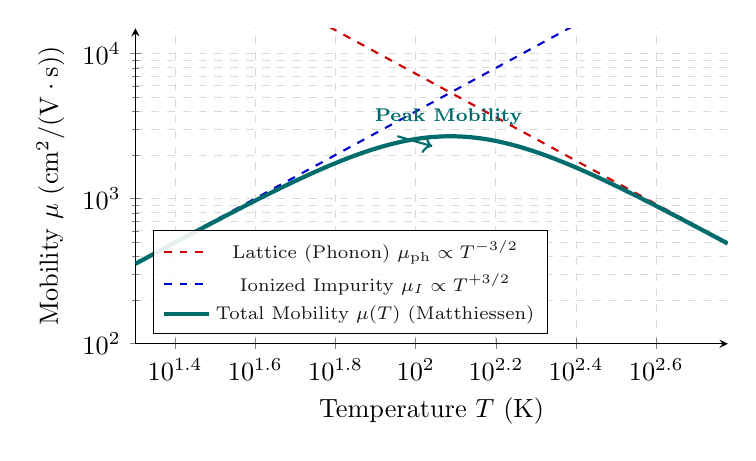
\begin{tikzpicture}[scale=0.95]
\begin{axis}[
    width=9.5cm, height=5.8cm,
    xmode=log, ymode=log,
    xmin=20, xmax=600,
    ymin=100, ymax=15000,
    xlabel={Temperature $T$ (K)},
    ylabel={Mobility $\mu$ ($\mathrm{cm^2/(V\cdot s)}$)},
    grid=both,
    grid style={dashed, gray!30},
    axis lines=left,
    legend pos=south west,
    legend style={font=\scriptsize, fill=white, fill opacity=0.9}
]
    \addplot[domain=20:600, samples=50, red!80!black, thick, dashed] {1400 * (300/x)^1.5};
    \addlegendentry{Lattice (Phonon) $\mu_{\mathrm{ph}} \propto T^{-3/2}$}

    \addplot[domain=20:600, samples=50, blue!80!black, thick, dashed] {4000 * (x/100)^1.5};
    \addlegendentry{Ionized Impurity $\mu_I \propto T^{+3/2}$}

    \addplot[domain=20:600, samples=80, teal!85!black, ultra thick] {1 / ( (1/(1400 * (300/x)^1.5)) + (1/(4000 * (x/100)^1.5)) )};
    \addlegendentry{Total Mobility $\mu(T)$ (Matthiessen)}

    \node[anchor=south west, font=\scriptsize\bfseries, teal!85!black] at (axis cs:75,2800) {Peak Mobility};
    \draw[->, thick, teal!85!black] (axis cs:90,2700) -- (axis cs:110,2300);
\end{axis}
\end{tikzpicture}
\caption{Temperature dependence of carrier mobility $\mu(T)$ in doped Silicon showing the crossover from ionized impurity scattering ($\mu \propto T^{3/2}$) at low temperatures to acoustic phonon scattering ($\mu \propto T^{-3/2}$) at high temperatures via Matthiessen's rule.}
\label{fig:mobility_temp_master}
\end{figure}

\subsection{The \texorpdfstring{$p$-$n$}{p-n} Junction: Band Alignment, Depletion Region, and Rectification \texorpdfstring{{\normalfont\normalsize\color{purple!75!black}\textbf{[Enrichment / Out of Syllabus]}}}{[Enrichment / Out of Syllabus]}}
\label{subsec:pn_junction}

\begin{enrichmentbox}{Course Syllabus Note}
\textbf{Syllabus Scope:} Electrostatics of the $p$-$n$ junction, space-charge depletion widths, and the Shockley diode equation represent advanced device applications beyond the core Module 4 examination syllabus.
\end{enrichmentbox}

\subsubsection{Contact Potential and Band Bending at Thermal Equilibrium}
When a $p$-type semiconductor ($p_{p0} \approx N_A$) and an $n$-type semiconductor ($n_{n0} \approx N_D$) form an abrupt metallurgical junction at $x=0$, enormous carrier concentration gradients exist across the interface:
\begin{itemize}[noitemsep]
    \item Majority holes in the $p$-region diffuse across $x=0$ into the $n$-region, leaving behind uncompensated, negatively charged acceptor cores ($N_A^-$).
    \item Majority electrons in the $n$-region diffuse across $x=0$ into the $p$-region, leaving behind uncompensated, positively charged donor cores ($N_D^+$).
\end{itemize}
The recombining electrons and holes leave a region of width $W = x_p + x_n$ around the interface completely stripped of mobile carriers: the \textbf{Space-Charge Region} (or \textbf{Depletion Region}).
The exposed fixed ionic cores create a built-in electric field $\bm{\mathcal{E}}$ pointing in the $-x$ direction (from $+n$ to $-p$), which exerts a drift force that opposes further diffusion.

In thermal equilibrium with no applied external bias, thermodynamic detailed balance requires the chemical potential (Fermi level $E_F$) to be perfectly flat and uniform across the entire device:
\begin{equation}
    \dv{E_F}{x} = 0 \implies E_{Fp} = E_{Fn} \equiv E_F.
\end{equation}
Because $E_F$ lies near $E_v$ on the $p$-side and near $E_c$ on the $n$-side, the conduction and valence band edges must bend continuously across the depletion region by an energy step equal to the \textbf{built-in potential energy} $e V_{bi}$ (Figure~\ref{fig:pn_junction_master}).

\subsubsection{Derivation of the Built-In Potential \texorpdfstring{$V_{bi}$}{Vbi}}
Deep in the neutral $n$-region ($x > x_n$), the electron concentration is $n_{n0} \approx N_D = N_c e^{-(E_c - E_F)/(k_B T)}$, which gives:
\begin{equation}
    E_c(n) - E_F = k_B T \ln\left(\frac{N_c}{N_D}\right).
\end{equation}
Deep in the neutral $p$-region ($x < -x_p$), the hole concentration is $p_{p0} \approx N_A = N_v e^{-(E_F - E_v)/(k_B T)}$, which gives:
\begin{equation}
    E_F - E_v(p) = k_B T \ln\left(\frac{N_v}{N_A}\right) \implies E_c(p) - E_F = E_g - k_B T \ln\left(\frac{N_v}{N_A}\right).
\end{equation}
Subtracting the two band-edge positions gives the total electrostatic energy step $e V_{bi}$:
\begin{align}
    e V_{bi} &= E_c(p) - E_c(n) = E_g - k_B T \ln\left(\frac{N_c N_v}{N_A N_D}\right) \nonumber \\
    &= k_B T \ln\left(\frac{N_c N_v e^{-E_g/(k_B T)}}{n_i^2} \frac{N_A N_D}{N_c N_v}\right) = k_B T \ln\left(\frac{N_A N_D}{n_i^2}\right).
\end{align}
Dividing by $e$ yields the \textbf{built-in potential} $V_{bi}$:
\begin{equation}
    \boxed{V_{bi} = \frac{k_B T}{e}\ln\left(\frac{N_A N_D}{n_i^2}\right) = V_T \ln\left(\frac{N_A N_D}{n_i^2}\right).}
    \label{eq:vbi_master}
\end{equation}
For a typical Silicon $p$-$n$ junction at $300\ \mathrm{K}$ ($n_i = 1.5\times 10^{10}\ \mathrm{cm^{-3}}$) with $N_A = 10^{16}\ \mathrm{cm^{-3}}$ and $N_D = 10^{17}\ \mathrm{cm^{-3}}$:
\begin{equation}
    V_{bi} = (0.02585\ \mathrm{V})\ln\left(\frac{10^{16} \times 10^{17}}{(1.5\times 10^{10})^2}\right) = (0.02585)\ln\left(4.44\times 10^{12}\right) = \mathbf{0.753\ \mathrm{V}}.
\end{equation}

\subsubsection{Space-Charge Distribution, Poisson's Equation, and Depletion Width \texorpdfstring{$W$}{W}}
In the \textbf{depletion approximation}, mobile carrier concentrations inside the space-charge layer $-x_p \le x \le x_n$ are assumed negligible compared to the dopant densities. The net charge density $\rho(x)$ is therefore:
\begin{equation}
    \rho(x) = \begin{cases}
        -e N_A, & -x_p \le x < 0 \quad (p\text{-side}) \\
        +e N_D, & 0 < x \le x_n \quad (n\text{-side}) \\
        0, & x < -x_p \text{ or } x > x_n \quad (\text{neutral regions}).
    \end{cases}
\end{equation}
Because the crystal as a whole remains strictly electrically neutral, the total negative acceptor charge on the $p$-side must balance the total positive donor charge on the $n$-side:
\begin{equation}
    e N_A x_p A = e N_D x_n A \implies \boxed{N_A x_p = N_D x_n.}
    \label{eq:charge_neutrality_pn}
\end{equation}
Eq.~\eqref{eq:charge_neutrality_pn} reveals a crucial design principle: \emph{the depletion region extends much farther into the more lightly doped semiconductor side}.

Integrating 1D Poisson's equation $\dv{\mathcal{E}}{x} = \frac{\rho(x)}{\epsilon_s}$ (where $\epsilon_s = \epsilon_r \epsilon_0$) subject to boundary conditions $\mathcal{E}(-x_p) = 0$ and $\mathcal{E}(x_n) = 0$:
\begin{equation}
    \mathcal{E}(x) = \begin{cases}
        -\frac{e N_A}{\epsilon_s}(x + x_p), & -x_p \le x \le 0, \\
        +\frac{e N_D}{\epsilon_s}(x - x_n), & 0 \le x \le x_n.
    \end{cases}
\end{equation}
The electric field is strictly negative (points in the $-x$ direction) and reaches its \textbf{maximum peak magnitude} right at the metallurgical interface $x = 0$:
\begin{equation}
    \boxed{\mathcal{E}_{\max} = \abs{\mathcal{E}(0)} = \frac{e N_A x_p}{\epsilon_s} = \frac{e N_D x_n}{\epsilon_s}.}
    \label{eq:emax_master}
\end{equation}

The total electrostatic potential drop across the junction under an applied external bias voltage $V$ (forward bias $V > 0$, reverse bias $V < 0$) equals the area under the triangular electric field profile:
\begin{equation}
    V_{bi} - V = -\int_{-x_p}^{x_n} \mathcal{E}(x)\,\dd x = \frac{1}{2}\mathcal{E}_{\max} (x_p + x_n) = \frac{e}{2\epsilon_s}\left(N_A x_p^2 + N_D x_n^2\right).
\end{equation}
Substituting $x_p = \frac{N_D}{N_A + N_D}W$ and $x_n = \frac{N_A}{N_A + N_D}W$ from Eq.~\eqref{eq:charge_neutrality_pn} (where $W = x_p + x_n$ is the total depletion width):
\begin{equation}
    V_{bi} - V = \frac{e}{2\epsilon_s} \frac{N_A N_D}{N_A + N_D} W^2.
\end{equation}
Solving for $W$ gives the fundamental \textbf{depletion width formula}:
\begin{equation}
    \boxed{W = \sqrt{\frac{2\epsilon_s}{e}\left(\frac{1}{N_A} + \frac{1}{N_D}\right)(V_{bi} - V)} = \sqrt{\frac{2\epsilon_s(N_A + N_D)}{e N_A N_D}(V_{bi} - V)}.}
    \label{eq:depletion_width_master}
\end{equation}
The individual depletion layer penetration depths into the $p$ and $n$ regions are:
\begin{equation}
    \boxed{x_p = W\left(\frac{N_D}{N_A + N_D}\right), \qquad x_n = W\left(\frac{N_A}{N_A + N_D}\right).}
\end{equation}
In a strongly asymmetric one-sided step junction ($p^+$-$n$, where $N_A \gg N_D$), virtually the entire depletion zone falls inside the lightly doped $n$-side:
\begin{equation}
    W \approx x_n \approx \sqrt{\frac{2\epsilon_s (V_{bi} - V)}{e N_D}}, \qquad \mathcal{E}_{\max} \approx \frac{2(V_{bi} - V)}{W}.
\end{equation}

\begin{figure}[htbp]
\centering
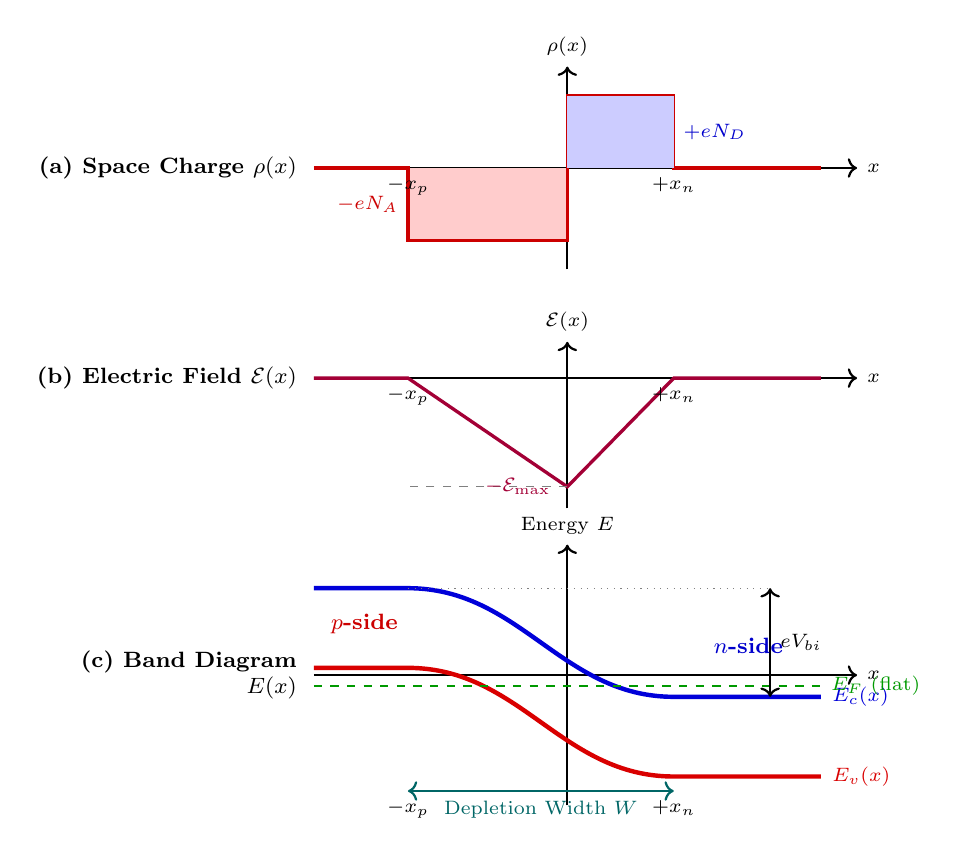
\begin{tikzpicture}[scale=0.92]
  % Panel (a): Charge density rho(x)
  \begin{scope}[shift={(0,5.2)}]
    \draw[->,thick] (-3.5,0) -- (4.0,0) node[right,font=\scriptsize] {$x$};
    \draw[->,thick] (0,-1.4) -- (0,1.4) node[above,font=\scriptsize] {$\rho(x)$};
    \fill[red!20] (-2.2,-1.0) rectangle (0,0);
    \draw[red!80!black,very thick] (-3.5,0) -- (-2.2,0) -- (-2.2,-1.0) -- (0,-1.0) -- (0,1.0) -- (1.47,1.0) -- (1.47,0) -- (3.5,0);
    \fill[blue!20] (0,0) rectangle (1.47,1.0);
    \node[left,font=\scriptsize,red!80!black] at (-2.2,-0.5) {$-e N_A$};
    \node[right,font=\scriptsize,blue!80!black] at (1.47,0.5) {$+e N_D$};
    \node[below,font=\scriptsize] at (-2.2,0) {$-x_p$};
    \node[below,font=\scriptsize] at (1.47,0) {$+x_n$};
    \node[left,font=\footnotesize\bfseries] at (-3.6,0) {(a) Space Charge $\rho(x)$};
  \end{scope}

  % Panel (b): Electric field E(x)
  \begin{scope}[shift={(0,2.3)}]
    \draw[->,thick] (-3.5,0) -- (4.0,0) node[right,font=\scriptsize] {$x$};
    \draw[->,thick] (0,-1.8) -- (0,0.5) node[above,font=\scriptsize] {$\mathcal{E}(x)$};
    \draw[very thick,purple!85!black] (-3.5,0) -- (-2.2,0) -- (0,-1.5) -- (1.47,0) -- (3.5,0);
    \draw[dashed,gray] (0,-1.5) -- (-2.2,-1.5);
    \node[left,font=\scriptsize,purple!85!black] at (-0.1,-1.5) {$-\mathcal{E}_{\max}$};
    \node[below,font=\scriptsize] at (-2.2,0) {$-x_p$};
    \node[below,font=\scriptsize] at (1.47,0) {$+x_n$};
    \node[left,font=\footnotesize\bfseries] at (-3.6,0) {(b) Electric Field $\mathcal{E}(x)$};
  \end{scope}

  % Panel (c): Energy Band Diagram
  \begin{scope}[shift={(0,-1.8)}]
    \draw[->,thick] (-3.5,0) -- (4.0,0) node[right,font=\scriptsize] {$x$};
    \draw[->,thick] (0,-1.8) -- (0,1.8) node[above,font=\scriptsize] {Energy $E$};
    
    % Ec curve
    \draw[ultra thick,blue!85!black] (-3.5,1.2) -- (-2.2,1.2) 
      to[out=0,in=180] (1.47,-0.3) -- (3.5,-0.3) node[right,font=\scriptsize] {$E_c(x)$};
      
    % Ev curve
    \draw[ultra thick,red!85!black] (-3.5,0.1) -- (-2.2,0.1) 
      to[out=0,in=180] (1.47,-1.4) -- (3.5,-1.4) node[right,font=\scriptsize] {$E_v(x)$};
      
    % Fermi level Ef
    \draw[dashed,thick,green!60!black] (-3.5,-0.15) -- (3.5,-0.15) node[right,font=\scriptsize] {$E_F$ (flat)};
    
    % Barrier eVbi
    \draw[<->,thick,black] (2.8,1.2) -- (2.8,-0.3) node[midway,right,font=\scriptsize] {$e V_{bi}$};
    \draw[dotted,gray] (-2.2,1.2) -- (2.8,1.2);
    
    \node[below,font=\scriptsize] at (-2.2,-1.6) {$-x_p$};
    \node[below,font=\scriptsize] at (1.47,-1.6) {$+x_n$};
    \draw[<->,thick,teal!80!black] (-2.2,-1.6) -- (1.47,-1.6) node[midway,below,font=\scriptsize] {Depletion Width $W$};
    
    \node[left,font=\footnotesize\bfseries,align=right] at (-3.6,0) {(c) Band Diagram\\$E(x)$};
    \node[font=\footnotesize\bfseries,red!80!black] at (-2.8,0.7) {$p$-side};
    \node[font=\footnotesize\bfseries,blue!80!black] at (2.5,0.4) {$n$-side};
  \end{scope}
\end{tikzpicture}
\caption{The abrupt $p$-$n$ step junction in thermal equilibrium: (a) space-charge density $\rho(x)$ exposing ionized cores, (b) triangular internal electric field $\mathcal{E}(x)$ peaking at $x=0$, and (c) energy band bending showing constant Fermi level $E_F$, band edges $E_c(x), E_v(x)$, and the built-in potential barrier $e V_{bi}$.}
\label{fig:pn_junction_master}
\end{figure}

\subsubsection{Non-Equilibrium Biased Junction and the Shockley Diode Equation}
Applying an external voltage bias $V$ across the terminals splits the Fermi level into two separate quasi-Fermi levels $E_{Fn}$ and $E_{Fp}$ ($E_{Fn} - E_{Fp} = e V$):
\begin{enumerate}
    \item \textbf{Forward Bias ($V > 0$, positive terminal connected to $p$-side):}
    The applied voltage lowers the electrostatic barrier from $V_{bi}$ to $V_{bi} - V$. The depletion width narrows according to $W(V) \propto \sqrt{V_{bi} - V}$. The lowered barrier enables majority electrons from the $n$-side and majority holes from the $p$-side to diffuse in massive numbers across the junction, injecting minority carriers into the quasi-neutral regions ($n_p(0) = n_{p0}e^{eV/(k_B T)}$ and $p_n(0) = p_{n0}e^{eV/(k_B T)}$). These excess minority carriers diffuse and recombine over characteristic \textbf{diffusion lengths} $L_n = \sqrt{D_n \tau_n}$ and $L_p = \sqrt{D_p \tau_p}$, producing a large forward current that grows exponentially with voltage.
    \item \textbf{Reverse Bias ($V < 0$, negative terminal connected to $p$-side):}
    The applied voltage raises the barrier from $V_{bi}$ to $V_{bi} + \abs{V}$. The depletion width expands: $W(V) \propto \sqrt{V_{bi} + \abs{V}}$. Diffusion of majority carriers over this towering barrier is completely suppressed. The only current that can flow is due to thermally generated minority carriers within a diffusion length of the depletion edges that get swept across by the strong electric field, producing a tiny, voltage-independent \textbf{reverse saturation current} $J_0$.
\end{enumerate}

Solving the steady-state minority carrier diffusion equations $\dvtwo{(\Delta n_p)}{x} = \frac{\Delta n_p}{L_n^2}$ and $\dvtwo{(\Delta p_n)}{x} = \frac{\Delta p_n}{L_p^2}$ in the neutral regions yields the celebrated \textbf{Shockley Ideal Diode Equation}:
\begin{equation}
    \boxed{J = J_0\left(e^{\frac{eV}{n_d k_B T}} - 1\right), \qquad I = I_0\left(e^{\frac{eV}{n_d k_B T}} - 1\right),}
    \label{eq:shockley_diode_master}
\end{equation}
where $n_d$ is the \textbf{diode ideality factor} ($n_d = 1.0$ for ideal diffusion transport, $n_d \approx 1\text{--}2$ in Silicon at low currents due to electron-hole recombination within the depletion region), and the \textbf{reverse saturation current density} is:
\begin{equation}
    \boxed{J_0 = e\left(\frac{D_n n_{p0}}{L_n} + \frac{D_p p_{n0}}{L_p}\right) = e n_i^2\left(\frac{D_n}{L_n N_A} + \frac{D_p}{L_p N_D}\right).}
    \label{eq:j0_master}
\end{equation}
Because $J_0 \propto n_i^2 \propto e^{-E_g/(k_B T)}$, semiconductors with larger band gaps exhibit dramatically smaller reverse leakage currents ($J_0 \sim 10^{-12}\ \mathrm{A/cm^2}$ in $\text{Si}$ versus $J_0 \sim 10^{-6}\ \mathrm{A/cm^2}$ in $\text{Ge}$ at $300\ \mathrm{K}$), making Silicon vastly superior for power rectification and logic switching.

% ============================================================================
\section{Comprehensive Solved Problems Bank (Exam Preparation)}
\label{sec:solved_bank}
% ============================================================================

\begin{examplebox}{Bloch Oscillations in a GaAs/AlGaAs Superlattice \textnormal{\color{purple!75!black}[Enrichment]}}{ex:bloch_superlattice}
\textbf{Problem.} A $\text{GaAs}/\text{AlGaAs}$ superlattice has period $d = 12.0\ \mathrm{nm}$ and miniband width $W = 4t = 35\ \mathrm{meV}$. An electric field $\mathcal{E} = 1.5\times 10^5\ \mathrm{V/m}$ is applied along the superlattice axis. Calculate (a) the Bloch frequency $f_B = \omega_B/(2\pi)$ and period $T_B$, (b) the real-space oscillation amplitude $L_B$, and (c) the maximum electron group velocity $v_{\max}$.
\vspace{0.2cm}\hrule\vspace{0.2cm}
\textbf{Solution.}
\textbf{(a)} $f_B = \frac{e\mathcal{E}d}{h} = \frac{(1.602\times 10^{-19}\ \mathrm{C})(1.5\times 10^5\ \mathrm{V/m})(12.0\times 10^{-9}\ \mathrm{m})}{6.626\times 10^{-34}\ \mathrm{J\cdot s}} = \mathbf{4.35\times 10^{11}\ \mathrm{Hz} = 0.435\ \mathrm{THz}}$, and $T_B = \frac{1}{f_B} = \mathbf{2.30\ \mathrm{ps}}$.\\
\textbf{(b)} $L_B = \frac{W}{e\mathcal{E}} = \frac{0.035\ \mathrm{eV}}{e(1.5\times 10^5\ \mathrm{V/m})} = \mathbf{2.33\times 10^{-7}\ \mathrm{m} = 233\ \mathrm{nm}}$ (approx.\ $19.4$ superlattice periods).\\
\textbf{(c)} Since $W = 4t = 35\ \mathrm{meV} \implies 2t = 17.5\ \mathrm{meV}$, $v_{\max} = \frac{2td}{\hb} = \frac{(17.5\times 10^{-3}\times 1.602\times 10^{-19}\ \mathrm{J})(12.0\times 10^{-9}\ \mathrm{m})}{1.055\times 10^{-34}\ \mathrm{J\cdot s}} = \mathbf{3.19\times 10^5\ \mathrm{m/s}}$.
\end{examplebox}

\begin{examplebox}{Donor Freeze-Out vs.\ Saturation Carrier Concentration}{ex:freezeout_calc}
\textbf{Problem.} An uncompensated Silicon sample ($\Delta E_d = 45\ \mathrm{meV}$, $m_e^* = 1.08\,m_e$) is doped with $N_d = 1.0\times 10^{16}\ \mathrm{cm^{-3}}$ phosphorus donors. Calculate the conduction electron concentration $n$ and Fermi level $E_c - E_F$ at (a) $T = 300\ \mathrm{K}$ and (b) $T = 40\ \mathrm{K}$ using the exact quadratic formula Eq.~\eqref{eq:quadratic_n_master}.
\vspace{0.2cm}\hrule\vspace{0.2cm}
\textbf{Solution.}
\textbf{(a) At $T = 300\ \mathrm{K}$:} $k_B T = 25.85\ \mathrm{meV}$ and $N_c(300\ \mathrm{K}) = 2.82\times 10^{19}\ \mathrm{cm^{-3}}$. Thus:
\[
    K_d(300\ \mathrm{K}) = \frac{1}{2}(2.82\times 10^{19})e^{-45/25.85} = 2.47\times 10^{18}\ \mathrm{cm^{-3}} \gg N_d.
\]
Hence $n(300\ \mathrm{K}) \approx N_d = \mathbf{9.96\times 10^{15}\ \mathrm{cm^{-3}}}$ (complete saturation), and $E_c - E_F = k_B T\ln(N_c/n) = \mathbf{0.205\ \mathrm{eV}}$.\\
\textbf{(b) At $T = 40\ \mathrm{K}$:} $k_B T = 3.447\ \mathrm{meV}$ and $N_c(40\ \mathrm{K}) = 2.82\times 10^{19}\times (40/300)^{3/2} = 1.37\times 10^{18}\ \mathrm{cm^{-3}}$. Thus:
\[
    K_d(40\ \mathrm{K}) = \frac{1}{2}(1.37\times 10^{18})e^{-45/3.447} = 1.48\times 10^{12}\ \mathrm{cm^{-3}} \ll N_d.
\]
Substituting into Eq.~\eqref{eq:quadratic_n_master} gives $n(40\ \mathrm{K}) \approx \sqrt{K_d N_d} = \sqrt{(1.48\times 10^{12})(1.0\times 10^{16})} = \mathbf{1.22\times 10^{14}\ \mathrm{cm^{-3}}}$ (only $1.22\%$ of donors are ionized — freeze-out regime!), and $E_c - E_F = (3.447\ \mathrm{meV})\ln\left(\frac{1.37\times 10^{18}}{1.22\times 10^{14}}\right) = \mathbf{32.1\ \mathrm{meV}}$.
\end{examplebox}

\begin{examplebox}{Zero Hall Coefficient Condition in an InSb Semiconductor}{ex:zero_hall}
\textbf{Problem.} In Indium Antimonide ($\text{InSb}$), the electron-to-hole mobility ratio is $b \equiv \mu_e/\mu_h = 80$, and the intrinsic carrier concentration at $300\ \mathrm{K}$ is $n_i = 2.0\times 10^{16}\ \mathrm{cm^{-3}}$. If the crystal is $p$-type doped with acceptors, find the hole concentration $p$, electron concentration $n$, and net acceptor concentration $N_a$ at which the Hall coefficient $R_H$ vanishes ($R_H = 0$).
\vspace{0.2cm}\hrule\vspace{0.2cm}
\textbf{Solution.}
From the two-carrier Hall formula Eq.~\eqref{eq:two_carrier_hall_master}, $R_H = 0$ when $p\mu_h^2 = n\mu_e^2 \implies p = n\left(\frac{\mu_e}{\mu_h}\right)^2 = b^2 n = 6400\,n$. Combining this with the Law of Mass Action $np = n_i^2$:
\begin{align*}
    n(6400\,n) = n_i^2 &\implies n = \frac{n_i}{80} = \frac{2.0\times 10^{16}\ \mathrm{cm^{-3}}}{80} = \mathbf{2.50\times 10^{14}\ \mathrm{cm^{-3}}}, \\
    &\implies p = 80\,n_i = \mathbf{1.60\times 10^{18}\ \mathrm{cm^{-3}}}.
\end{align*}
By charge neutrality ($p - n = N_a$), the required acceptor doping is $N_a = p - n \approx \mathbf{1.60\times 10^{18}\ \mathrm{cm^{-3}}}$.
\end{examplebox}

\begin{examplebox}{Kronig--Penney Model Allowed Bandwidth for Potential Strength $P = 3\pi/2$}{ex:kp_p3}
\textbf{Problem.} In the Dirac-delta Kronig--Penney model, the dispersion relation is given by $P\frac{\sin(\alpha a)}{\alpha a} + \cos(\alpha a) = \cos(ka)$. Let the barrier strength be $P = \frac{3\pi}{2} \approx 4.712$. Find:
\begin{enumerate}[noitemsep]
    \item the energy of the band bottom ($k = 0$) of the lowest energy band,
    \item the energy of the band top ($k = \pi/a$) of the lowest energy band,
    \item the allowed bandwidth $W_1$ in units of $E_1 \equiv \frac{\pi^2\hb^2}{2ma^2}$, and
    \item the width of the first forbidden energy gap $\Delta E_{g1}$ between the first and second allowed bands.
\end{enumerate}
\vspace{0.2cm}\hrule\vspace{0.2cm}
\textbf{Solution.}
Defining the dimensionless parameter $\xi \equiv \alpha a = \sqrt{\frac{2mE}{\hb^2}}a$, energy is related to $\xi$ by $E = \left(\frac{\xi}{\pi}\right)^2 E_1$.\\
\textbf{(a)} At the band bottom ($k = 0$), $\cos(ka) = 1$:
\[
    f(\xi) \equiv \frac{P\sin\xi}{\xi} + \cos\xi = 1 \implies \frac{(3\pi/2)\sin\xi}{\xi} + \cos\xi = 1.
\]
Solving numerically for the lowest positive root gives $\xi_{\min} \approx \mathbf{1.905\ \mathrm{rad}}$ ($= 0.6063\,\pi$). Thus:
\[
    E_{\min} = \left(\frac{1.905}{\pi}\right)^2 E_1 = (0.6063)^2 E_1 = \mathbf{0.3676\,E_1}.
\]
\textbf{(b)} At the band top ($k = \pi/a$), $\cos(ka) = -1$:
\[
    f(\xi) = \frac{P\sin\xi}{\xi} + \cos\xi = -1.
\]
Notice that at $\xi = \pi$, $\sin\pi = 0$ and $\cos\pi = -1$, so $f(\pi) = -1$ \emph{identically for all values of $P$}! Therefore, the top of the lowest band is exactly:
\[
    \xi_{\max} = \pi \implies E_{\max} = \left(\frac{\pi}{\pi}\right)^2 E_1 = \mathbf{1.0000\,E_1}.
\]
\textbf{(c)} The allowed bandwidth of the lowest band is:
\[
    W_1 = E_{\max} - E_{\min} = 1.0000\,E_1 - 0.3676\,E_1 = \mathbf{0.6324\,E_1}.
\]
\textbf{(d)} The bottom of the second band corresponds to the next root of $f(\xi) = -1$ with $\xi > \pi$. Setting $\xi = \pi + \delta$, numerical solution gives $\xi_2 \approx \mathbf{3.964\ \mathrm{rad}} = 1.2618\,\pi$. Hence the bottom of the second band is:
\[
    E_2 = (1.2618)^2 E_1 = \mathbf{1.5921\,E_1}.
\]
The first forbidden energy gap is therefore:
\[
    \Delta E_{g1} = E_2 - E_{\max} = 1.5921\,E_1 - 1.0000\,E_1 = \mathbf{0.5921\,E_1}.
\]
\end{examplebox}

\begin{examplebox}{1D Tight-Binding Bandwidth, Effective Mass, and Maximum Velocity}{ex:tb_prob_solved}
\textbf{Problem.} A one-dimensional crystal lattice has lattice constant $a = 3.0\ \text{\AA} = 3.0\times 10^{-10}\ \mathrm{m}$ and nearest-neighbor hopping matrix element $t = 1.0\ \mathrm{eV}$ ($1.602\times 10^{-19}\ \mathrm{J}$), with atomic site energy $\epsilon_0 = 0$.
\begin{enumerate}[noitemsep]
    \item Calculate the total bandwidth $W$.
    \item Calculate the effective mass $m^*(k)$ at the band bottom ($k = 0$) and at the band top ($k = \pi/a$) in units of the bare electron rest mass $m_e$.
    \item Calculate the maximum electron group velocity $v_{\max}$ and specify the wavevector $k$ at which it occurs.
\end{enumerate}
\vspace{0.2cm}\hrule\vspace{0.2cm}
\textbf{Solution.}
From the tight-binding dispersion $E(k) = -2t\cos(ka)$:\\
\textbf{(a)} The bandwidth is:
\[
    W = E\left(\frac{\pi}{a}\right) - E(0) = (+2t) - (-2t) = 4t = 4(1.0\ \mathrm{eV}) = \mathbf{4.0\ \mathrm{eV}}.
\]
\textbf{(b)} The inverse effective mass is $\frac{1}{m^*(k)} = \frac{1}{\hb^2}\dvtwo{E}{k} = \frac{2ta^2}{\hb^2}\cos(ka) \implies m^*(k) = \frac{\hb^2}{2ta^2\cos(ka)}$.
At the band bottom ($k = 0$):
\[
    m^*(0) = +\frac{\hb^2}{2ta^2} = \frac{(1.0546\times 10^{-34}\ \mathrm{J\cdot s})^2}{2(1.6022\times 10^{-19}\ \mathrm{J})(3.0\times 10^{-10}\ \mathrm{m})^2} = \mathbf{3.856\times 10^{-31}\ \mathrm{kg}} = \mathbf{0.423\,m_e}.
\]
At the band top ($k = \pi/a$):
\[
    m^*(\pi/a) = -\frac{\hb^2}{2ta^2} = \mathbf{-3.856\times 10^{-31}\ \mathrm{kg}} = \mathbf{-0.423\,m_e} \quad (\implies m_h^* = +0.423\,m_e).
\]
\textbf{(c)} The group velocity is $v_g(k) = \frac{1}{\hb}\dv{E}{k} = \frac{2ta}{\hb}\sin(ka)$. The maximum velocity occurs at the inflection point $k = \pm\frac{\pi}{2a}$ where $\sin(ka) = 1$:
\[
    v_{\max} = \frac{2ta}{\hb} = \frac{2(1.6022\times 10^{-19}\ \mathrm{J})(3.0\times 10^{-10}\ \mathrm{m})}{1.0546\times 10^{-34}\ \mathrm{J\cdot s}} = \mathbf{9.117\times 10^5\ \mathrm{m/s}}.
\]
\end{examplebox}

\begin{examplebox}{Carrier Drift Transport, Conductivity, and Diffusion Length in Silicon}{ex:drift_diff_solved}
\textbf{Problem.} An uncompensated $n$-type Silicon bar at $300\ \mathrm{K}$ is doped with phosphorus donors at $N_d = 2.0\times 10^{16}\ \mathrm{cm^{-3}}$. The electron and hole mobilities are $\mu_n = 1350\ \mathrm{cm^2/(V\cdot s)}$ and $\mu_p = 460\ \mathrm{cm^2/(V\cdot s)}$, and the minority hole recombination lifetime is $\tau_p = 1.2\ \mu\mathrm{s}$. The sample has length $L = 0.50\ \mathrm{cm}$ and cross-sectional area $A = 0.040\ \mathrm{cm^2}$. A DC voltage $V = 5.0\ \mathrm{V}$ is applied across its length.
Calculate:
\begin{enumerate}[noitemsep]
    \item the longitudinal electric field $\mathcal{E}$ and the terminal drift velocities $v_{d,n}$ and $v_{d,p}$,
    \item the electrical conductivity $\sigma$, resistivity $\rho$, and total drift current $I$,
    \item the electron and hole diffusion coefficients $D_n$ and $D_p$ using the Einstein relation, and
    \item the minority carrier diffusion length $L_p$.
\end{enumerate}
\vspace{0.2cm}\hrule\vspace{0.2cm}
\textbf{Solution.}
\textbf{(a)} The electric field is $\mathcal{E} = \frac{V}{L} = \frac{5.0\ \mathrm{V}}{0.50\ \mathrm{cm}} = \mathbf{10.0\ \mathrm{V/cm} = 1.00\times 10^3\ \mathrm{V/m}}$.
The drift velocities are:
\[
    \abs{v_{d,n}} = \mu_n \mathcal{E} = (1350\ \mathrm{cm^2/(V\cdot s)})(10.0\ \mathrm{V/cm}) = \mathbf{1.35\times 10^4\ \mathrm{cm/s} = 135\ \mathrm{m/s}},
\]
\[
    \abs{v_{d,p}} = \mu_p \mathcal{E} = (460\ \mathrm{cm^2/(V\cdot s)})(10.0\ \mathrm{V/cm}) = \mathbf{4.60\times 10^3\ \mathrm{cm/s} = 46.0\ \mathrm{m/s}}.
\]
\textbf{(b)} In the saturation range at $300\ \mathrm{K}$, $n \approx N_d = 2.0\times 10^{16}\ \mathrm{cm^{-3}}$, while minority holes are $p = n_i^2/N_d = (1.5\times 10^{10})^2 / (2.0\times 10^{16}) = 1.125\times 10^4\ \mathrm{cm^{-3}} \ll n$. Thus:
\begin{align*}
    \sigma &\approx e n \mu_n = (1.602\times 10^{-19}\ \mathrm{C})(2.0\times 10^{16}\ \mathrm{cm^{-3}})(1350\ \mathrm{cm^2/(V\cdot s)}) \\
           &= \mathbf{4.325\ \Omega^{-1}\mathrm{cm^{-1}} = 432.5\ \Omega^{-1}\mathrm{m^{-1}}},
\end{align*}
\[
    \rho = \frac{1}{\sigma} = \mathbf{0.231\ \Omega\cdot\mathrm{cm} = 2.31\times 10^{-3}\ \Omega\cdot\mathrm{m}}.
\]
The sample resistance is $R = \rho \frac{L}{A} = (0.231\ \Omega\cdot\mathrm{cm})\frac{0.50\ \mathrm{cm}}{0.040\ \mathrm{cm^2}} = 2.89\ \Omega$. The total current is:
\[
    I = \frac{V}{R} = \frac{5.0\ \mathrm{V}}{2.89\ \Omega} = \mathbf{1.73\ \mathrm{A}}.
\]
\textbf{(c)} By the Einstein relation with $V_T = \frac{k_B T}{e} = 0.02585\ \mathrm{V}$ at $300\ \mathrm{K}$:
\[
    D_n = \mu_n V_T = (1350\ \mathrm{cm^2/(V\cdot s)})(0.02585\ \mathrm{V}) = \mathbf{34.90\ \mathrm{cm^2/s} = 3.490\times 10^{-3}\ \mathrm{m^2/s}},
\]
\[
    D_p = \mu_p V_T = (460\ \mathrm{cm^2/(V\cdot s)})(0.02585\ \mathrm{V}) = \mathbf{11.89\ \mathrm{cm^2/s} = 1.189\times 10^{-3}\ \mathrm{m^2/s}}.
\]
\textbf{(d)} The minority hole diffusion length is:
\begin{align*}
    L_p &= \sqrt{D_p \tau_p} = \sqrt{(11.89\ \mathrm{cm^2/s})(1.2\times 10^{-6}\ \mathrm{s})} \\
        &= \sqrt{1.427\times 10^{-5}\ \mathrm{cm^2}} = \mathbf{3.78\times 10^{-3}\ \mathrm{cm} = 37.8\ \mu\mathrm{m}}.
\end{align*}
\end{examplebox}

\begin{examplebox}{Built-in Potential, Depletion Width, and Peak Electric Field in a Si $p$-$n$ Junction \textnormal{\color{purple!75!black}[Enrichment]}}{ex:pn_junction_solved}
\textbf{Problem.} An abrupt Silicon $p$-$n$ step junction at $T = 300\ \mathrm{K}$ ($n_i = 1.5\times 10^{10}\ \mathrm{cm^{-3}}$, $\epsilon_r = 11.7$, $\epsilon_0 = 8.854\times 10^{-14}\ \mathrm{F/cm}$) has acceptor doping $N_A = 2.0\times 10^{16}\ \mathrm{cm^{-3}}$ on the $p$-side and donor doping $N_D = 1.0\times 10^{17}\ \mathrm{cm^{-3}}$ on the $n$-side.
Calculate:
\begin{enumerate}[noitemsep]
    \item the built-in contact potential $V_{bi}$,
    \item the total depletion width $W$ and individual penetration depths $x_p$ and $x_n$ at equilibrium ($V = 0$),
    \item the peak maximum internal electric field $\mathcal{E}_{\max}$ at equilibrium, and
    \item the total depletion width $W$ under a reverse bias voltage of $V_R = 5.0\ \mathrm{V}$ ($V = -5.0\ \mathrm{V}$).
\end{enumerate}
\vspace{0.2cm}\hrule\vspace{0.2cm}
\textbf{Solution.}
The semiconductor permittivity is $\epsilon_s = \epsilon_r \epsilon_0 = (11.7)(8.854\times 10^{-14}\ \mathrm{F/cm}) = 1.036\times 10^{-12}\ \mathrm{F/cm}$.\\
\textbf{(a)} The built-in potential is:
\begin{align*}
    V_{bi} &= V_T \ln\left(\frac{N_A N_D}{n_i^2}\right) = (0.02585\ \mathrm{V})\ln\left(\frac{(2.0\times 10^{16})(1.0\times 10^{17})}{(1.5\times 10^{10})^2}\right) \\
           &= (0.02585)\ln(8.889\times 10^{12}) = \mathbf{0.771\ \mathrm{V}}.
\end{align*}
\textbf{(b)} At zero bias ($V = 0$):
\begin{align*}
    W &= \sqrt{\frac{2\epsilon_s}{e}\left(\frac{N_A + N_D}{N_A N_D}\right)V_{bi}} \\
      &= \sqrt{\frac{2(1.036\times 10^{-12}\ \mathrm{F/cm})}{1.602\times 10^{-19}\ \mathrm{C}}\left(\frac{1.2\times 10^{17}\ \mathrm{cm^{-3}}}{2.0\times 10^{33}\ \mathrm{cm^{-6}}}\right)(0.771\ \mathrm{V})} \\
      &= \sqrt{5.983\times 10^{-10}\ \mathrm{cm^2}} = \mathbf{2.45\times 10^{-5}\ \mathrm{cm} = 0.245\ \mu\mathrm{m} = 245\ \mathrm{nm}}.
\end{align*}
The individual depletion layer penetration depths are:
\[
    x_p = W\left(\frac{N_D}{N_A + N_D}\right) = (0.245\ \mu\mathrm{m})\left(\frac{1.0\times 10^{17}}{1.2\times 10^{17}}\right) = \mathbf{0.204\ \mu\mathrm{m} = 204\ \mathrm{nm}},
\]
\[
    x_n = W\left(\frac{N_A}{N_A + N_D}\right) = (0.245\ \mu\mathrm{m})\left(\frac{2.0\times 10^{16}}{1.2\times 10^{17}}\right) = \mathbf{0.041\ \mu\mathrm{m} = 41\ \mathrm{nm}}.
\]
(Notice that $x_p/x_n = N_D/N_A = 5$: the depletion layer is 5 times wider on the lightly doped $p$-side!)\\
\textbf{(c)} The maximum peak electric field at $x = 0$ is:
\[
    \mathcal{E}_{\max} = \frac{2 V_{bi}}{W} = \frac{2(0.771\ \mathrm{V})}{2.45\times 10^{-5}\ \mathrm{cm}} = \mathbf{6.29\times 10^4\ \mathrm{V/cm} = 6.29\times 10^6\ \mathrm{V/m}}.
\]
\textbf{(d)} Under reverse bias $V = -V_R = -5.0\ \mathrm{V}$, the total potential drop is $V_{bi} + V_R = 0.771 + 5.0 = 5.771\ \mathrm{V}$. Since $W \propto \sqrt{V_{bi} - V}$:
\begin{align*}
    W(V = -5\ \mathrm{V}) &= W(0)\sqrt{\frac{V_{bi} + V_R}{V_{bi}}} = (0.245\ \mu\mathrm{m})\sqrt{\frac{0.771 + 5.0}{0.771}} \\
    &= (0.245\ \mu\mathrm{m})\sqrt{7.485} = \mathbf{0.670\ \mu\mathrm{m} = 670\ \mathrm{nm}}.
\end{align*}
\end{examplebox}

\end{document}